% ============================================================
% TESIS DOCTORAL
% Eficiencia hospitalaria, estructura organizativa
% y teoría de agencia: Un análisis de frontera estocástica
% del sistema hospitalario español
%
% José María Elena Izquierdo
% Departamento de Economía Aplicada
% Universidad de Salamanca
% 2026
% ============================================================

\documentclass[12pt, a4paper, twoside, openright]{book}

% ── Codificación y lengua ───────────────────────────────────
\usepackage[utf8]{inputenc}
\usepackage[T1]{fontenc}
\usepackage[spanish,es-nodecimaldot]{babel}

% ── Tipografía ──────────────────────────────────────────────
\usepackage{lmodern}
\usepackage{microtype}

% ── Matemáticas ─────────────────────────────────────────────
\usepackage{amsmath, amssymb, amsthm, amsfonts}
\usepackage{bm}

% ── Tablas y figuras ────────────────────────────────────────
\usepackage{booktabs}
\usepackage{longtable}
\usepackage{array}
\usepackage{multirow}
\usepackage{threeparttable}
\usepackage{tabularx}
\usepackage{rotating}
\usepackage{pdflscape}
\usepackage{graphicx}
\usepackage{caption}
\usepackage{subcaption}
\usepackage{float}

% ── Diseño de página ────────────────────────────────────────
\usepackage{geometry}
\geometry{
  top=2.5cm, bottom=2.5cm,
  left=3.5cm, right=2.5cm,
  bindingoffset=0.5cm,
  headheight=28pt
}
\usepackage{setspace}
\onehalfspacing

% ── Encabezados y pies ──────────────────────────────────────
\usepackage{fancyhdr}
\pagestyle{fancy}
\fancyhf{}
\fancyhead[LE]{\small\itshape\leftmark}
\fancyhead[RO]{\small\itshape\rightmark}
\fancyfoot[C]{\thepage}
\renewcommand{\headrulewidth}{0.4pt}

% ── Color (necesario para hyperref con colores mixtos) ──────
\usepackage[dvipsnames,svgnames,x11names]{xcolor}

% ── Referencias y enlaces ──────────────────────────────────
\usepackage[colorlinks=true,
  linkcolor={blue!60!black},
  citecolor={blue!60!black},
  urlcolor={blue!60!black}]{hyperref}
\usepackage{natbib}
\usepackage{eurosym}

% ── Figuras: ruta hacia directorio teórico ─────────────────
\graphicspath{{../Teórico/}{./}}

% ── Diagramas TikZ ──────────────────────────────────────────
\usepackage{tikz}
\usetikzlibrary{arrows.meta, positioning, shapes.geometric}

% ── Otros ───────────────────────────────────────────────────
\usepackage{color,soul}
\usepackage{enumitem}
\usepackage{footnote}

% ── Comandos propios ────────────────────────────────────────
\newcommand{\E}{\mathbb{E}}
\newcommand{\N}{\mathcal{N}}
\newcommand{\e}{\mathrm{e}}
\newcommand{\bsym}[1]{\boldsymbol{#1}}
\newcommand{\sig}[1]{\ensuremath{^{#1}}}

% ── Entornos de teorema ─────────────────────────────────────
\theoremstyle{plain}
\newtheorem{proposition}{Proposición}[chapter]
\newtheorem{result}{Resultado}[chapter]
\newtheorem{corollary}{Corolario}[chapter]
\theoremstyle{definition}
\newtheorem{definition}{Definición}[chapter]
\theoremstyle{remark}
\newtheorem{remark}{Observación}[chapter]

% ═══════════════════════════════════════════════════════════
\begin{document}
% ═══════════════════════════════════════════════════════════

% ── PORTADA ─────────────────────────────────────────────────
\begin{titlepage}
\centering
\vspace*{2cm}

{\large UNIVERSIDAD DE SALAMANCA}\\[0.3cm]
{\normalsize Departamento de Economía Aplicada}\\[0.3cm]
{\normalsize Programa de Doctorado en Economía}

\vspace{2.5cm}

{\LARGE\bfseries Eficiencia hospitalaria, estructura\\[0.3cm]
organizativa y teoría de agencia}\\[0.6cm]
{\Large\itshape Un análisis de frontera estocástica\\
del sistema hospitalario español}

\vspace{2.5cm}

{\large Tesis Doctoral}

\vspace{1.5cm}

{\large José María Elena Izquierdo}

\vfill

{\normalsize Salamanca, 2026}
\end{titlepage}

% ── PÁGINAS PRELIMINARES ────────────────────────────────────
\frontmatter

\chapter*{Agradecimientos}
\addcontentsline{toc}{chapter}{Agradecimientos}
% [Pendiente de redacción]
\vspace{2cm}
\begin{center}
\textit{[Pendiente de redacción]}
\end{center}

\tableofcontents
\listoftables
\listoffigures

% ═══════════════════════════════════════════════════════════
\mainmatter
% ═══════════════════════════════════════════════════════════



% ###########################################################
% CAPÍTULO 1: INTRODUCCIÓN
% ###########################################################
\chapter{Introducción}
\label{ch:intro}

\section{Motivación y contexto}

La provisión de servicios hospitalarios constituye uno de los componentes más complejos y costosos de cualquier sistema sanitario. En España, el gasto hospitalario representa aproximadamente el 60\% del gasto sanitario público total \citep{oecd2023}, y el debate sobre la eficiencia de los hospitales ha cobrado renovada importancia en un contexto de restricción presupuestaria, envejecimiento poblacional y transformación tecnológica.

La complejidad del hospital como organización productiva reside en la multiplicidad de agentes que intervienen en la producción de servicios sanitarios: financiadores públicos, gestores hospitalarios, médicos, personal de enfermería y otros profesionales. Las acciones y esfuerzos combinados de estos agentes determinan tanto el volumen de atención prestada como su calidad e intensidad diagnóstico-terapéutica. Esta multiplicidad de agentes y tareas genera problemas de información asimétrica ---riesgo moral, selección adversa y observabilidad imperfecta del esfuerzo--- que están en el núcleo de la teoría de la agencia \citep{laffont2002,bolton2005}.

El sistema hospitalario español ofrece un laboratorio natural particularmente rico para el estudio de estas cuestiones. Aunque la estructura hospitalaria pública del Sistema Nacional de Salud (SNS) es la forma predominante de provisión, en las últimas décadas ha aumentado la participación de formas organizativas descentralizadas: concesiones administrativas, fundaciones sanitarias, empresas públicas y hospitales privados concertados \citep{repullo2008}. Esta diversidad institucional coexiste con variaciones en los mecanismos de pago ---desde el presupuesto global retrospectivo hasta los contratos-programa con pago prospectivo por actividad--- y con diferencias sustanciales en el grado de autonomía de los gestores hospitalarios para contratar y retribuir al personal médico.

La pregunta central de esta investigación es cómo la estructura organizativa del hospital ---centralizada o descentralizada--- afecta a la eficiencia productiva en las distintas dimensiones del output hospitalario. La hipótesis fundamental, derivada del modelo teórico de \citet{izquierdo2019}, es que los efectos de la descentralización no son simétricos: la autonomía en la gestión de contratos e incentivos permite a los hospitales descentralizados mejorar su eficiencia en la producción de volumen (cantidad de altas), pero puede simultáneamente reducir su eficiencia en la dimensión de intensidad diagnóstico-terapéutica, debido a la sustitución de esfuerzo entre tareas que los incentivos de volumen inducen en el comportamiento del médico.

\section{Marco teórico: agencia y multitarea en hospitales}

La aplicación de la teoría de la agencia al sector sanitario tiene una larga tradición que se remonta al trabajo seminal de \citet{arrow1963} sobre la incertidumbre y la economía del bienestar médico. En el contexto hospitalario, los modelos de agencia se han centrado en las relaciones entre financiadores y proveedores \citep{ellis1986,mcclellan1997}, entre hospitales y médicos \citep{ma1997,jelovac2002} y, más recientemente, en configuraciones multinivel que reconocen la jerarquía de relaciones contractuales inherente a la organización hospitalaria.

El modelo de multitarea de \citet{holmstrom1991} proporcionó el marco analítico fundamental para comprender cómo la presencia de múltiples dimensiones del output afecta al diseño óptimo de incentivos. En un entorno multitarea, la potencia de los incentivos sobre una dimensión del output debe calibrarse teniendo en cuenta su efecto sobre las demás dimensiones: si las tareas son sustitutas en la función de costes del agente, un incentivo fuerte sobre una tarea induce un desplazamiento de esfuerzo desde las otras. Este resultado tiene implicaciones directas para la financiación hospitalaria, donde el pago por actividad (incentivo de volumen) puede deteriorar la calidad o la intensidad del tratamiento si ambas dimensiones compiten por el tiempo y el esfuerzo del médico \citep{eggleston2005,kaarboe2011}.

La literatura sobre la relación entre estructura organizativa y eficiencia hospitalaria ha abordado la cuestión desde perspectivas complementarias. En el terreno teórico, \citet{jelovac2002} analizan los contratos óptimos para hospital y médico bajo riesgo moral bilateral, identificando las condiciones bajo las cuales la contratación centralizada domina a la descentralizada y viceversa. \citet{chalkley1998} estudian los contratos óptimos entre financiadores y hospitales cuando la calidad es imperfectamente observable, mostrando que esquemas mixtos de pago fijo y variable pueden dominar a los esquemas puros. \citet{ma1994} analiza los incentivos de coste y calidad generados por distintos sistemas de pago hospitalario, mostrando que ningún mecanismo domina a todos los demás en todas las dimensiones. \citet{eggleston2005} examina cómo la interacción entre el tipo de pago y la estructura organizativa afecta a la provisión de calidad en sistemas multihospitalarios.

En el terreno empírico, la eficiencia hospitalaria se ha estudiado extensamente mediante técnicas de frontera ---tanto paramétricas (análisis de frontera estocástica, SFA) como no paramétricas (análisis envolvente de datos, DEA). Entre los trabajos de referencia para el contexto español, \citet{puigjunoy2000} estiman una frontera de costes estocástica con datos del SIAE, encontrando niveles de ineficiencia significativos y asociados al tamaño y la complejidad del hospital. \citet{prior2006} analiza la eficiencia de hospitales catalanes mediante DEA, documentando diferencias significativas entre hospitales públicos y concertados. A escala internacional, \citet{zuckerman1994} estiman fronteras de costes para hospitales estadounidenses; \citet{linna1998} aplica SFA a hospitales finlandeses identificando economías de escala; \citet{rosko2008} revisan críticamente las aplicaciones de SFA hospitalario. \citet{jacobs2006} y \citet{hollingsworth2008} proporcionan revisiones exhaustivas de la literatura de eficiencia hospitalaria, abarcando más de doscientos estudios.

La relación entre propiedad hospitalaria y eficiencia ha generado una literatura específica. \citet{newhouse1970} propuso el modelo teórico seminal del hospital sin ánimo de lucro. \citet{sloan2000} revisa la evidencia sobre comportamiento de los hospitales sin ánimo de lucro en el \textit{Handbook of Health Economics}. Para el contexto europeo, \citet{herr2011} analiza la eficiencia técnica y de costes de hospitales alemanes según titularidad, y \citet{tiemann2012} estudian los efectos de la privatización. Estas evidencias son relevantes para la interpretación de los resultados del presente trabajo, dado que la variable $D^{desc}$ captura parcialmente la propiedad, aunque no se identifica con ella. Para una perspectiva de organización industrial, \citet{gaynor2015} proporcionan una revisión comprehensiva de los mercados sanitarios.

Sin embargo, la conexión entre la teoría de la agencia y la estimación empírica de la eficiencia ha recibido escasa atención. La mayoría de los trabajos empíricos estiman fronteras sin un modelo teórico que genere predicciones específicas sobre los determinantes de la ineficiencia, o bien formulan predicciones ad hoc sin derivación formal. Esta brecha entre la teoría de la agencia aplicada al sector sanitario y la literatura empírica de eficiencia hospitalaria ha sido señalada por \citet{hollingsworth2008} como uno de los déficits más importantes de la literatura. Esta tesis pretende llenar ese vacío: el modelo teórico de \citet{izquierdo2019} genera predicciones contrastables y falsificables sobre cómo la estructura organizativa y el mecanismo de pago afectan diferencialmente a la eficiencia en las dos dimensiones del output hospitalario, y la parte empírica contrasta esas predicciones con datos de panel del sistema hospitalario español.

La literatura de eficiencia hospitalaria ha crecido sustancialmente en las últimas dos décadas, impulsada por la disponibilidad de datos administrativos de alta calidad y por el desarrollo de técnicas econométricas de frontera. \citet{worthington2004} revisa 80 estudios de eficiencia hospitalaria publicados entre 1983 y 2002 y documenta una gran heterogeneidad en los métodos y resultados. \citet{hollingsworth2008} actualiza esa revisión con 317 estudios de eficiencia sanitaria (incluyendo hospitales, centros de atención primaria y sistemas de salud) y concluye que la eficiencia técnica media en los estudios SFA de hospitales se sitúa alrededor del 0.83, con un rango amplio entre estudios. La diferencia entre nuestros valores medios (0.68--0.79) y este benchmark puede explicarse parcialmente por el período de mayor restricción presupuestaria analizado (2010--2023 incluye los años de mayor austeridad del SNS) y por el uso de fronteras separadas por dimensión del output.

Los trabajos que se aproximan más al enfoque de esta tesis son los que vinculan explícitamente los determinantes institucionales con la ineficiencia técnica a través de modelos de un paso (\textit{one-step models}) \citep{battese1995,wang2002}. \citet{burgess1998} estiman la variación en ineficiencia entre hospitales estadounidenses atribuyéndola a diferencias en la presión competitiva del mercado local. \citet{farsi2005} analizan la eficiencia técnica y de costes en hospitales suizos, identificando efectos diferenciales de la propiedad y el tamaño. \citet{herr2011} estudia la eficiencia técnica en hospitales alemanes con distintas formas de propiedad. Ninguno de estos trabajos, sin embargo, tiene como punto de partida un modelo de agencia que genere predicciones específicas sobre los determinantes de la ineficiencia en múltiples dimensiones del output.

\section{Objetivos y contribución}

Los objetivos de esta tesis son tres:

\begin{enumerate}[label=(\roman*)]
  \item Desarrollar un modelo teórico de agencia multitarea que caracterice las relaciones contractuales entre financiador, hospital y médico bajo riesgo moral, y que genere predicciones contrastables sobre los efectos diferenciales de la estructura organizativa en las dos dimensiones del output hospitalario.

  \item Diseñar y ejecutar una estrategia empírica que permita contrastar esas predicciones utilizando técnicas de frontera estocástica (SFA) con datos de panel del sistema hospitalario español para el período 2010--2023.

  \item Derivar implicaciones de política sanitaria sobre el diseño de la estructura organizativa y los mecanismos de pago a hospitales, fundamentadas tanto en la teoría como en la evidencia empírica.
\end{enumerate}

La contribución de esta tesis es cuádruple.

En primer lugar, en el plano teórico, el modelo de \citet{izquierdo2019} extiende los resultados clásicos de la teoría de multitarea \citep{holmstrom1991} al caso de tres agentes y dos outputs producidos asimétricamente, derivando predicciones sobre la interacción entre estructura organizativa, tipo de pago y complementariedad/sustitución entre tareas que, hasta donde conocemos, no están disponibles en la literatura previa. En particular, el resultado de que la potencia de los incentivos del hospital sea función de $\psi_{12}$ en la estructura descentralizada pero no en la centralizada (potencia secuencialmente inducida) es una contribución analítica nueva.

En segundo lugar, en el plano empírico, la estimación de un sistema de dos fronteras estocásticas ---una para cada dimensión del output--- constituye la primera contrastación empírica directa de un modelo de agencia multitarea en el sector hospitalario español. El diseño empírico permite identificar si los efectos de la descentralización son efectivamente de signo opuesto (o al menos asimétricos) entre la cantidad y la intensidad, algo que un modelo con un único término de ineficiencia no puede captar. La confirmación de P4 en el Diseño B con $z_{dif}=-9.89$ ($p<0.001$) es el resultado empírico más sólido y directamente vinculado al mecanismo teórico.

En tercer lugar, en el plano metodológico, la tesis contribuye a la literatura de SFA hospitalario al proporcionar cuatro diseños complementarios de estimación ---función de distancia output, sistema bivariado cantidad/intensidad, sistema bivariado quirúrgico/médico y panel hospital$\times$servicio--- que explotan distintas fuentes de variación y permiten una triangulación de los resultados. Esta estrategia de triangulación es replicable y extensible a otros sistemas sanitarios con datos de estructura similar.

En cuarto lugar, en el plano de datos, la construcción del panel armonizado del sistema hospitalario español para 2010--2023, integrando SIAE, CNH y CMBD parcial con imputación de case-mix mediante aprendizaje automático, constituye un activo de investigación disponible para análisis posteriores. El pipeline de datos documentado en el Anexo~\ref{app:pipeline} está diseñado para ser reproducible y actualizable con los datos de años futuros del SIAE.

\section{El sistema hospitalario español: contexto institucional}
\label{sec:contexto_sns}

\subsection{Estructura del SNS tras las transferencias autonómicas}

El Sistema Nacional de Salud español, configurado por la Ley General de Sanidad de 1986, descansa sobre tres principios: universalidad, equidad y financiación pública. Hasta el año 2002, varias comunidades autónomas gestionaban ya sus propias redes hospitalarias (Cataluña desde 1981, Andalucía desde 1984, País Vasco y la Comunidad Valenciana desde 1987, Navarra desde 1990 y Galicia y las Islas Canarias desde 1994). La reforma del sistema de financiación autonómica aprobada en 2001 y efectiva en 2002 completó el proceso de transferencias sanitarias al conjunto de las comunidades autónomas, poniendo fin al INSALUD como gestor directo de los servicios sanitarios en las comunidades que permanecían bajo gestión central.

El resultado es un sistema descentralizado en el que diecisiete servicios autonómicos de salud ejercen la función de compradores de servicios hospitalarios dentro de sus respectivos territorios \citep{repullo2008}. Esta estructura descentralizada ha generado una creciente heterogeneidad tanto en los modelos organizativos de los hospitales como en los mecanismos de pago y contratación del personal sanitario, haciendo del sistema hospitalario español un objeto de análisis especialmente rico para la economía de la salud.

\subsection{Tipología de hospitales del sistema español}

La diversidad organizativa del sistema hospitalario español puede clasificarse en cinco grandes categorías según la dependencia funcional y el régimen de gestión:

\begin{enumerate}[label=(\roman*)]
  \item \textbf{Hospitales públicos integrados del SNS:} Constituyen la columna vertebral del sistema. El personal es estatutario (funcionario o laboral especial) y las condiciones de contratación están sujetas al Estatuto Marco del personal estatutario de los servicios de salud (Ley 55/2003). La financiación proviene del presupuesto del servicio autonómico de salud, generalmente mediante contratos-programa anuales que establecen objetivos de actividad y calidad. El hospital no tiene autonomía para fijar libremente retribuciones ni para despedir personal.

  \item \textbf{Fundaciones sanitarias públicas:} Surgieron en los años noventa como fórmula para introducir flexibilidad de gestión manteniendo la titularidad pública. Los trabajadores tienen contratos laborales ordinarios, lo que permite al hospital adaptar las plantillas y retribuciones con mayor agilidad. Galicia y Cataluña fueron las comunidades pioneras en este modelo. La eficiencia de las fundaciones sanitarias gallegas ha sido analizada por \citet{prior2006} y otros autores que encuentran resultados mixtos en comparación con los hospitales integrados.

  \item \textbf{Empresas públicas hospitalarias:} Sociedad mercantil de capital íntegramente público, con mayor autonomía de gestión. El modelo típico es la Empresa Pública de Emergencias Sanitarias o los hospitales creados bajo la Ley de Agencias Públicas Empresariales andaluza. La relación laboral es mercantil, lo que amplía la capacidad del hospital para incentivar al personal.

  \item \textbf{Concesiones administrativas (modelo Alzira):} La Comunidad Valenciana introdujo en 1999 la concesión administrativa del hospital de La Ribera (Alzira) a una empresa privada (inicialmente Adeslas-Ribera Salud), que asumía tanto la gestión hospitalaria como la atención primaria de su área de salud a cambio de una tarifa capitativa pactada por habitante y año. Este modelo, extendido posteriormente a otros hospitales valencianos (Torrevieja, Dénia, Manises, Vinalopó) y adaptado en la Comunidad de Madrid (Hospital de Majadahonda, Hospital del Sureste), representa el máximo grado de descentralización: el contratista privado diseña autónomamente los contratos del personal médico y fija las retribuciones variables. Los hospitales gestionados bajo concesión administrativa son el caso empíricamente más limpio de estructura descentralizada en el sentido del modelo teórico.

  \item \textbf{Hospitales privados concertados:} Hospitales de titularidad privada (con o sin ánimo de lucro) que prestan servicios al SNS mediante contratos de concierto. El hospital recibe una tarifa pactada por acto o estancia y mantiene plena autonomía para contratar y retribuir al personal. La Fundación Jiménez Díaz (Madrid), los hospitales de la red concertada catalana (XHUP) y numerosos centros de congregaciones religiosas son los ejemplos más representativos.
\end{enumerate}

\subsection{Evolución reciente: expansión y reversión de concesiones}

El período 2003--2012 fue la fase de mayor expansión de los modelos de gestión privada. La Comunidad de Madrid aprobó la construcción de ocho nuevos hospitales bajo el modelo de colaboración público-privada (CPP), donde la empresa privada construye y gestiona los servicios no sanitarios, mientras el personal clínico sigue siendo estatutario. Aunque este modelo es menos descentralizado que las concesiones valencianas, amplió significativamente la participación privada en la red hospitalaria madrileña.

A partir de 2012, la crisis económica y el cambio de ciclo político iniciaron un proceso de reversión. La Comunidad Valenciana anunció en 2018 la reversión del hospital de Alzira al sistema público una vez expirada la concesión, argumentando que el ahorro de costes era modesto y que el modelo había generado problemas de continuidad asistencial. En 2021, otros hospitales de la red valenciana completaron su integración en la red pública. La Comunidad de Madrid, por su parte, revirtió en 2015 el proceso de privatización de seis hospitales después de que el Tribunal Superior de Justicia de Madrid suspendiera cautelarmente el proceso de licitación. Estas reversiones han generado un debate académico sobre los efectos de la estructura organizativa en la eficiencia que esta tesis pretende contribuir a iluminar con evidencia empírica rigurosa.

\subsection{Mecanismos de pago hospitalario en España}

Los mecanismos de pago al hospital son un determinante central de los incentivos de eficiencia, tal como enfatiza el modelo teórico. En el sistema hospitalario español coexisten tres grandes mecanismos:

\begin{enumerate}[label=(\alph*)]
  \item \textbf{Presupuesto global retrospectivo:} Típico de los hospitales públicos integrados en la etapa anterior a los contratos-programa. El hospital recibe una asignación presupuestaria global, con escasa vinculación a la actividad realizada. Este esquema equivale al pago fijo del modelo teórico: los incentivos de volumen son débiles o inexistentes.

  \item \textbf{Contratos-programa con pago por actividad (GRD):} A partir de los años noventa, los servicios autonómicos de salud empezaron a vincular parte de la financiación hospitalaria a la actividad, utilizando los Grupos Relacionados por el Diagnóstico (GRD) como unidad de medida de la complejidad del caso. El contrato-programa establece un volumen de actividad objetivo y una tarifa por GRD; los hospitales que superan el objetivo reciben una compensación adicional (a menudo a tarifa marginal reducida). En algunas comunidades autónomas (Cataluña, Comunidad Valenciana, País Vasco), este sistema de pago por actividad está relativamente desarrollado y se extiende también a los hospitales concertados.

  \item \textbf{Capitación ajustada:} Las concesiones administrativas de tipo Alzira se financian mediante una tarifa capitativa anual ajustada por el estado de salud de la población del área. Este mecanismo de pago crea incentivos radicalmente distintos a los anteriores: el hospital tiene incentivos para reducir la utilización por episodio (eficiencia en intensidad) y para mantener a la población sana (prevención y atención primaria).
\end{enumerate}

Esta diversidad de mecanismos de pago se refleja en la variable $pct^{SNS}$ del modelo empírico: los hospitales con alta dependencia del SNS están sujetos predominantemente a financiación pública por actividad, mientras que los hospitales privados de mercado con baja dependencia del SNS operan bajo esquemas de pago directo o de seguros privados.

\subsection{Datos básicos del sistema hospitalario español}

El sistema hospitalario español comprende, en el período analizado (2010--2023), aproximadamente 880 hospitales con internamiento registrados en el SIAE, de los cuales algo más de 400 son hospitales de agudos activos con actividad suficiente para la estimación. El número de camas en funcionamiento ha disminuido levemente en el período, de aproximadamente 145.000 en 2010 a 137.000 en 2019 (excluyendo el período COVID). El gasto hospitalario público representó en 2019 alrededor del 5.7\% del PIB, equivalente a unos 68.000 millones de euros \citep{oecd2023}.

La distribución entre hospitales públicos integrados y el resto es aproximadamente 60/40 en términos de número de hospitales y 75/25 en términos de altas totales, lo que refleja el mayor tamaño medio de los hospitales públicos. La Comunidad de Madrid y Cataluña concentran el mayor número de hospitales privados concertados, mientras que la distribución de concesiones se concentraba en la Comunidad Valenciana hasta las reversiones de 2018--2021.

\section{Justificación metodológica: SFA versus DEA}
\label{sec:justificacion_metodologica}

\subsection{Por qué análisis de frontera estocástica}

La medición de la eficiencia hospitalaria puede abordarse mediante dos grandes familias de técnicas: el análisis envolvente de datos (DEA), de naturaleza no paramétrica, y el análisis de frontera estocástica (SFA), de naturaleza paramétrica \citep{coelli2005}. La elección de SFA en esta tesis no es arbitraria; está justificada por cuatro razones metodológicas y una sustantiva.

\textit{Primera}, el SFA distingue explícitamente entre ineficiencia técnica y ruido estadístico. Dado que los datos hospitalarios contienen errores de medición sustanciales ---en particular en las variables de output como las altas ponderadas por case-mix--- mezclar ruido e ineficiencia produciría estimaciones sesgadas. El DEA no tiene término de error aleatorio: toda desviación de la frontera se atribuye a ineficiencia. El SFA descompone la desviación en $v_{it}$ (ruido) y $u_{it}$ (ineficiencia), lo que es más apropiado cuando la variable de output es una medida imperfecta del output verdadero \citep{aigner1977,meeusen1977,kumbhakar2000}.

\textit{Segunda}, la disponibilidad de datos de panel para el período 2010--2023 permite explotar la variación temporal dentro del hospital para identificar los efectos de los determinantes de la ineficiencia. El SFA de panel con efectos heterogéneos en la media de la distribución de ineficiencia \citep{battese1995,wang2002} es el marco natural para este análisis. Las extensiones de panel del DEA (DEA de Malmquist) no permiten incorporar covariables de la ineficiencia de forma tan directa.

\textit{Tercera}, el SFA produce errores estándar para los coeficientes de la ecuación de ineficiencia, lo que permite contrastar formalmente las predicciones del modelo teórico (tests $t$, LR, Kodde-Palm). El DEA no tiene distribución muestral conocida para los índices de eficiencia, aunque \citet{simar2007} propone métodos de bootstrap; sin embargo, estos métodos no están disponibles para modelos con covariables en la ecuación de ineficiencia de panel. Para una presentación exhaustiva de las opciones de estimación SFA, véanse \citet{kumbhakar2000} y \citet{greene2008}.

\textit{Cuarta}, la función de producción translog especificada en el Capítulo~\ref{ch:estrategia} tiene una justificación económica directa: permite testar restricciones de curvatura (simetría de las segundas derivadas, rendimientos de escala), estimar elasticidades de sustitución y verificar la consistencia con la teoría de la producción. El DEA no impone ninguna estructura paramétrica a la tecnología, lo que es una ventaja general pero en este contexto específico supone renunciar a las restricciones teóricas que el modelo justifica.

\textit{La razón sustantiva} es que el objetivo del análisis no es simplemente clasificar hospitales por eficiencia, sino contrastar predicciones de un modelo teórico sobre los determinantes de la ineficiencia. Para ello se necesita un modelo paramétrico que vincule las variables institucionales (estructura organizativa, mecanismo de pago, interacción entre tareas) con la distribución de la ineficiencia a través de una ecuación de media heterogénea. Este tipo de análisis es genuinamente SFA.

\subsection{Ventajas del panel sobre la sección cruzada}

El uso de datos de panel (2010--2023) frente a una sección cruzada tiene ventajas sustanciales en el contexto de esta investigación. \textit{Primera}, permite separar la heterogeneidad no observada permanente del hospital de la ineficiencia transitoria \citep{greene2005a}. Un hospital que siempre opera por debajo de la frontera puede reflejar diferencias tecnológicas permanentes (calidad del equipamiento, localización, cartera de servicios) más que ineficiencia propiamente dicha. \textit{Segunda}, la variación temporal en la variable $D^{desc}$ ---derivada principalmente de los cambios en la dependencia funcional registrada en el CNH y de las entradas y salidas de hospitales de la muestra--- proporciona identificación adicional del efecto causal de la estructura organizativa sobre la ineficiencia. \textit{Tercera}, el panel permite estimar tendencias de progreso técnico ($t$ y $t^2$ en la frontera) y controlar cambios macro que afectan a todos los hospitales simultáneamente (reformas regulatorias, crisis económica, COVID).

\subsection{Justificación de la forma funcional translog}

La forma funcional translog \citep{zuckerman1994,linna1998} es la estándar en la literatura de eficiencia hospitalaria por tres razones. \textit{Primera}, es una aproximación de segundo orden a cualquier función de producción continua, sin imponer restricciones apriorísticas sobre la curvatura. Esto es importante en hospitales, donde las economías de escala y la complementariedad entre inputs son difícilmente conocidas \textit{ex ante}. \textit{Segunda}, a diferencia de la especificación Cobb-Douglas, permite que las elasticidades de los inputs varíen con el nivel de los inputs, lo que es empíricamente relevante cuando la muestra incluye hospitales muy heterogéneos en tamaño (de 50 a más de 2.000 camas). \textit{Tercera}, los tests de razón de verosimilitud reportados en la Tabla~\ref{tab:tests_spec} rechazan la Cobb-Douglas frente a la translog en los cuatro diseños de estimación con estadísticos entre 247 y 594.

\section{Estructura de la tesis}

La tesis se organiza del siguiente modo. El Capítulo~\ref{ch:modelo} presenta el modelo teórico de agencia multitarea: el planteamiento del juego, la solución de primer \textit{best}, los resultados bajo riesgo moral en estructuras centralizadas y descentralizadas, y las predicciones contrastables derivadas del equilibrio. Las simulaciones numéricas detalladas se presentan en el Anexo~\ref{app:simulaciones}, aunque las conclusiones principales se resumen en el cuerpo del capítulo.

El Capítulo~\ref{ch:estrategia} desarrolla la estrategia empírica: el marco del análisis de frontera estocástica, la especificación de la frontera de producción y de la ecuación de ineficiencia, y los cuatro diseños de estimación con sus respectivos roles en el análisis.

El Capítulo~\ref{ch:datos} describe los datos y las variables: las fuentes de información (SIAE, CNH, CMBD), la construcción de las variables principales y la muestra de estimación.

El Capítulo~\ref{ch:resultados} presenta los resultados principales de los cuatro diseños de estimación y los tests formales de hipótesis.

El Capítulo~\ref{ch:robustez} reporta los análisis de robustez, los tests de especificación y una discusión detallada de la interpretación económica de los resultados.

El Capítulo~\ref{ch:politica} deriva implicaciones de política hospitalaria a partir de los resultados teóricos y empíricos.

El Capítulo~\ref{ch:conclusiones} recoge las conclusiones generales, las limitaciones de la investigación y las líneas de extensión futura.



% ###########################################################
% CAPÍTULO 2: MODELO TEÓRICO
% ###########################################################
\chapter{Modelo teórico: incentivos y estructura organizativa en la financiación hospitalaria}
\label{ch:modelo}

\section{Introducción}

La financiación hospitalaria eficiente depende de los arreglos organizativos establecidos entre los distintos agentes que interactúan en la provisión de servicios sanitarios. En este capítulo estudiamos cómo, bajo riesgo moral, diferentes estructuras organizativas moldean el papel de los mecanismos de pago por incentivos para los médicos y los directivos hospitalarios.

La provisión de servicios hospitalarios es, en última instancia, el resultado de la interacción de múltiples agentes. Los financiadores ---públicos o privados--- compran servicios a los hospitales. Los gestores toman continuamente decisiones sobre la asignación de recursos humanos y materiales. Dentro de cada hospital, una multiplicidad de profesionales ---médicos, personal de enfermería, auxiliares, farmacéuticos--- realizan tareas distintas cuyas acciones combinadas determinan el conjunto de diagnósticos y procedimientos terapéuticos que intentan mejorar el estado de salud de los pacientes.

La importancia de la multiplicidad de tareas y agentes implicados ha sido estudiada en numerosos trabajos académicos centrados en los efectos sobre la eficiencia de distintos esquemas de financiación. \citet{jelovac2002}, en un enfoque cercano al nuestro, estudian los contratos óptimos tanto para el médico como para el hospital bajo riesgo moral bilateral, analizando las condiciones bajo las cuales es óptimo utilizar contratación centralizada o una estructura descentralizada en la que el principal delega en el hospital el diseño del contrato del médico. \citet{ma1997} analiza el papel de la información asimétrica en la relación médico-hospital y sus implicaciones para la eficiencia. \citet{eggleston2005} examina las consecuencias de distintas formas de pago sobre la calidad cuando hay múltiples agentes. \citet{kaarboe2011} estudian los incentivos del médico hospitalario en un entorno multitarea con información asimétrica.

Las regulaciones legales y administrativas del sistema sanitario influyen de manera fundamental en el funcionamiento de los incentivos. En el caso español, aunque la estructura hospitalaria pública es la forma predominante de provisión, ha aumentado la participación de organizaciones privadas y sin ánimo de lucro junto con las colaboraciones público-privadas \citep{repullo2008}. Más allá de las diferentes estructuras legales, hay una distinción esencial en la que se centra nuestro análisis: el grado de autonomía del que disfrutan los gestores hospitalarios al contratar sus insumos.

En los hospitales públicos del SNS, la autoridad sanitaria regional contrata de forma centralizada y simultánea tanto los servicios hospitalarios como a los miembros del personal. En los hospitales privados y sin ánimo de lucro, los gestores disponen de mayor margen de maniobra a la hora de elegir a los médicos que trabajarán en sus centros y de diseñar los esquemas retributivos internos. Además, cuando los hospitales tienen una dependencia funcional privada o no lucrativa, se utilizan con mayor frecuencia esquemas de pago del tipo \textit{fee-for-service}, mientras que en los hospitales públicos el financiador recurre más a menudo a remuneraciones salariales fijas.

Con este propósito, en las secciones siguientes desarrollamos un modelo teórico de riesgo moral con múltiples tareas bajo diferentes estructuras organizativas, derivando las restricciones de compatibilidad de incentivos y sus implicaciones sobre la potencia óptima de los incentivos y la eficiencia productiva. El objetivo último es obtener predicciones empíricamente contrastables que puedan aplicarse al sistema hospitalario español.


\section{Planteamiento del modelo}
\label{sec:planteamiento}

En el modelo interactúan tres agentes. En primer lugar, el asegurador de servicios sanitarios (el principal), que puede ser público o privado. Después, el consejo de dirección del hospital (el hospital, en adelante) y, finalmente, el médico. Hospital y médico producen conjuntamente dos outputs.

\subsection{Los dos outputs y su asimetría}

La primera dimensión del output es la \textbf{cantidad} de servicios sanitarios. Esta dimensión cuantitativa es el resultado de las interacciones de esfuerzo de hospital y médico:
\begin{equation}
  q(a,t_1)=a+t_1+\epsilon_1
  \label{eq:q}
\end{equation}
El escalar no negativo $a$ representa el esfuerzo del hospital para producir un cierto nivel de cantidad (por ejemplo, número de ingresos). El esfuerzo del médico dedicado a la cantidad viene dado por $t_1 \geq 0$. Los valores concretos de ambas variables, junto con un shock aleatorio $\epsilon_1$, determinan la cantidad.

La segunda dimensión es la \textbf{intensidad} (utilizada como aproximación de la calidad),\footnote{El concepto de calidad es escurridizo cuando se consideran los servicios hospitalarios; por ello nos centramos en la intensidad de los servicios diagnóstico-terapéuticos por paciente.} dada por:
\begin{equation}
  i(t_2)=t_2+\epsilon_2
  \label{eq:i}
\end{equation}
Esta variable es el resultado del esfuerzo del médico $t_2$ y de un shock aleatorio $\epsilon_2$. El hospital puede influir en la cantidad de altas hospitalarias pero no en la cantidad de servicios diagnósticos o terapéuticos por paciente, una decisión que recae exclusivamente en el médico.

El vector de output es $\bm{x}=(q,i)$. Los componentes aleatorios $\bm{\epsilon}=(\epsilon_1, \epsilon_2)$ se distribuyen normalmente con media cero y matriz de varianzas y covarianzas:
\begin{equation}
  \Sigma=\begin{pmatrix}
    \sigma^2_1 & \sigma^2_{12} \\
    \sigma^2_{12} & \sigma^2_2
  \end{pmatrix}
  \label{eq:sigma}
\end{equation}
es decir, $\bm{\epsilon}\sim N(\mathbf{0},\Sigma)$.

\begin{remark}
Esta asimetría en la producción es el núcleo estructural del modelo. Si ambos outputs fueran producidos por los mismos agentes con los mismos incentivos, las predicciones serían simétricas y no habría hipótesis falsificable sobre el efecto diferencial de la estructura organizativa. La asimetría en la producción refleja una realidad institucional del hospital: el médico es el agente con conocimiento privado sobre la idoneidad y la intensidad del tratamiento, mientras que el hospital (la dirección) tiene mayor control sobre la capacidad instalada y el flujo de pacientes. Esta distinción es análoga a la distinción entre esfuerzo de \textit{throughput} (volumen de actividad) y esfuerzo de \textit{quality} (intensidad por episodio) en la literatura de economía de la salud \citep{eggleston2005,kaarboe2011}.
\end{remark}

\subsection{Preferencias de los agentes}

La utilidad de los distintos agentes viene dada por:
\begin{align}
    u_f &= s(q,i)-\lambda[b(q,i)+w(q,i)] \label{eq:util_f}\\
    u_h(b,a) &= u_h[b(q,i)-\tau(a)+z(a)] \label{eq:util_h}\\
    u_m(w,t_1,t_2) &= u_m[w(q,i)-\psi(t_1,t_2)+\phi(t_1,t_2)] \label{eq:util_m}
\end{align}
donde $s(q,i)$ es la utilidad directa para el financiador de contratar $q$ e $i$, $b(q,i)$ es el pago al hospital y $w(q,i)$ la renta pagada al médico. Tanto el hospital como el médico asumen costes de ejercer sus respectivos niveles de esfuerzo ($\tau(a)$ y $\psi(t_1,t_2)$). Finalmente, se permiten preferencias altruistas o vocacionales, dependientes del esfuerzo, tanto en el hospital ($z(a)$) como en el médico ($\phi(t_1,t_2)$).

\subsection{El parámetro clave: \texorpdfstring{$\psi_{12}$}{psi\_12}}

La función de costes del médico $\psi(t_1,t_2)$ incorpora un parámetro de interacción entre tareas $\psi_{12}$ que mide el grado de complementariedad o sustituibilidad:
\begin{itemize}[leftmargin=2cm]
  \item Si $\psi_{12} > 0$ (tareas sustitutas): el médico que dedica más tiempo a ver pacientes reduce la intensidad que dedica a cada uno. Es el caso típico de servicios médicos no quirúrgicos.
  \item Si $\psi_{12} < 0$ (tareas complementarias): el acto de intervenir genera per se mayor intensidad. Es el caso típico de servicios quirúrgicos.
  \item Si $\psi_{12} = 0$: las tareas son independientes en la función de costes del médico.
\end{itemize}

Como se verá en la sección empírica, $\psi_{12}$ no es directamente observable. En la estimación se aproxima mediante la proporción de altas quirúrgicas sobre el total ($ShareQ$) a nivel de hospital-año, o bien se identifica de forma estructural separando los outputs quirúrgico y médico.


\section{La solución de primer \texorpdfstring{\textit{best}}{best}}
\label{sec:primer_best}

Cuando el principal tiene información completa sobre los esfuerzos de ambos agentes y contrata bajo una estructura centralizada,\footnote{Bajo información completa y estructura descentralizada, el principal implementará los mismos niveles de esfuerzo de primer \textit{best}, de modo que no es necesario comparar entre estructuras.} el problema de optimización es:
\begin{align*}
    \max_{a,t_1,t_2}\ \E_{\bm{\epsilon}}[u_f] &= \E_{\bm{\epsilon}}\left[s(q,i)-\lambda[b(q)+w(q,i)]\right]\\
    \text{s.a.}\quad \E_{\bm{\epsilon}}[u_h] &\geq u_h(\bar{b})\\
    \E_{\bm{\epsilon}}[u_m] &\geq u_m(\bar{w})
\end{align*}
donde $u_h(\bar{b})$ y $u_m(\bar{w})$ son las utilidades de reserva del hospital y del médico.\footnote{Dada la información completa, el principal no condiciona el pago de cada agente al esfuerzo del otro.}

El principal puede contratar el nivel óptimo de esfuerzos ($a^*,t^*_1,t^*_2$) y hacer vinculante la restricción de participación con pagos de suma fija:
\begin{align}
  b(q) = H &= \bar{b}+\tau(a^*)-z(a^*) \label{eq:pago_h_fb}\\
  w(q,i) = M &= \bar{w}+\psi(t_1^*,t_2^*)-\phi(t_1^*,t_2^*) \label{eq:pago_m_fb}
\end{align}

Las condiciones necesarias de primer orden del problema reducido son:
\begin{align}
  s_q+\lambda z_a &= \lambda\tau_a \label{eq:cpo1}\\
  s_q+\lambda\phi_{t_1} &= \lambda\psi_{t_1} \label{eq:cpo2}\\
  s_i+\lambda\phi_{t_2} &= \lambda\psi_{t_2} \label{eq:cpo3}
\end{align}

Combinando las ecuaciones~\eqref{eq:cpo1} y~\eqref{eq:cpo2}:
\begin{equation}
    \tau_a-z_a=\psi_{t_1}-\phi_{t_1}
    \label{eq:cpo_q}
\end{equation}
y las ecuaciones~\eqref{eq:cpo2} y~\eqref{eq:cpo3}:
\begin{equation}
  \frac{s_q}{s_i}=\frac{\psi_{t_1}-\phi_{t_1}}{\psi_{t_2}-\phi_{t_2}}=\frac{\tau_a-z_a}{\psi_{t_2}-\phi_{t_2}}
  \label{eq:cpo_qi}
\end{equation}

\begin{result}[Primer \textit{best}]
La ecuación~\eqref{eq:cpo_q} establece que los costes marginales netos de altruismo de ambos agentes al producir cantidad deben igualarse. La ecuación~\eqref{eq:cpo_qi} requiere que la tasa marginal de sustitución para el principal entre ambos outputs sea igual a la tasa marginal técnica de transformación entre cantidad e intensidad. Con estas condiciones se obtienen los niveles de esfuerzo de primer \textit{best} del médico en ambas tareas y, dado su esfuerzo óptimo en cantidad, el esfuerzo del hospital.
\end{result}

Una implicación relevante es que, si un hospital público o sin ánimo de lucro tiene un componente vocacional más alto ($z(a)$ mayor), entonces en el óptimo el principal debería exigirle un nivel de esfuerzo mayor: el principal explota el beneficio que el agente obtiene de su altruismo. Del mismo modo, si el único agente con preocupación directa por el bienestar del paciente es el médico ($z(a)=0$), entonces la ecuación~\eqref{eq:cpo_qi} implica que el principal contratará un mayor nivel de esfuerzo en intensidad respecto a la cantidad en comparación con el caso de un hospital con componente altruista.


\section{Riesgo moral bajo estructura centralizada}
\label{sec:centralizada}

De forma más realista, el principal no es capaz de verificar los esfuerzos de los agentes y debe utilizar el nivel de output como señal ruidosa del esfuerzo realizado. Siguiendo a \citet{holmstrom1991}, especificamos funciones de utilidad exponenciales (CARA) para los agentes, neutralidad al riesgo del principal ($s(q,i)=q+i$) y esquemas lineales de reembolso.

\subsection{Especificación funcional}

Las funciones de utilidad son:
\begin{align}
  u_h(b,a) &= -\e^{-\rho[b(q,i)-\tau(a)+z(a)]} \label{eq:util_h_cara}\\
  u_m(w,t_1,t_2) &= -\e^{-\eta[w(q,i)-\psi(t_1,t_2)+\phi(t_1,t_2)]} \label{eq:util_m_cara}
\end{align}
donde $\rho$ y $\eta$ son los coeficientes de aversión absoluta al riesgo del hospital y del médico \citep{holmstrom1987}.

Las funciones de coste del esfuerzo son:
\begin{align}
  \tau(a) &= \frac{1}{2}\tau a^2, \quad \tau>0 \label{eq:coste_h}\\
  \psi(t_1,t_2) &= \frac{1}{2}(\psi_1t_1^2+\psi_2t_2^2)+\psi_{12}t_1t_2, \quad \psi_1>0,\ \psi_2>0,\ \psi_{12}^2 \leq \psi_1\psi_2 \label{eq:coste_m}
\end{align}
El parámetro $\psi_{12}$ mide la interacción entre tareas.\footnote{Si $\psi_{12}^2=\psi_1\psi_2$, las tareas son sustitutivas perfectas. Si $\psi_{12}=0$, son independientes. Si $\psi_{12}<0$, son complementarias.}

El componente altruista sigue una especificación lineal:
\begin{align}
  z(a) &= z_1 a, \quad z_1 \geq 0 \label{eq:altruismo_h}\\
  \phi(t_1,t_2) &= \phi_1 t_1+\phi_2 t_2, \quad \phi_1, \phi_2 \geq 0 \label{eq:altruismo_m}
\end{align}

Los esquemas lineales de compensación son:
\begin{align}
  b(q) &= f+bq \label{eq:pago_h_lineal}\\
  w(q,i) &= F+Bq+Di \label{eq:pago_m_lineal}
\end{align}
donde $f$ y $F$ son los componentes fijos, y $b$, $B$ y $D$ son los componentes variables (incentivos) por cantidad e intensidad respectivamente.

La secuencia temporal de la contratación bajo estructura centralizada se representa en la Figura~\ref{fig:cronograma_c}. El principal ofrece contratos simultáneamente al hospital y al médico (etapa 1); ambos eligen sus niveles de esfuerzo (etapa 2); se realizan los outputs $q$ e $i$ (etapa 3); y se efectúan los pagos (etapa 4).

\begin{figure}[htbp]
  \centering
\begin{tikzpicture}[
    scale=0.95,
    every node/.style={font=\small},
    stage/.style={draw, rounded corners=3pt, fill=gray!10,
                  text width=2.9cm, align=center,
                  minimum height=1.6cm, inner sep=5pt},
    arrow/.style={-Stealth, thick}
]
  % Línea de tiempo
  \draw[thick] (0,0) -- (13.2,0);

  % Etapa 1
  \node[stage] (s1) at (1.65,0) {%
    \textbf{Etapa 1}\\[3pt]
    \footnotesize El Principal ofrece contratos al Hospital
    ($b(q)$) y al Médico ($w(q,i)$)
  };

  % Etapa 2
  \node[stage] (s2) at (4.95,0) {%
    \textbf{Etapa 2}\\[3pt]
    \footnotesize Hospital y Médico aceptan o rechazan;
    eligen esfuerzos $a$, $t_1$, $t_2$
  };

  % Etapa 3
  \node[stage] (s3) at (8.25,0) {%
    \textbf{Etapa 3}\\[3pt]
    \footnotesize La Naturaleza determina los outputs
    $q$ e $i$ (observables con ruido)
  };

  % Etapa 4
  \node[stage] (s4) at (11.55,0) {%
    \textbf{Etapa 4}\\[3pt]
    \footnotesize Se realizan los pagos $b(q)$ al Hospital
    y $w(q,i)$ al Médico
  };

  % Marcas de tiempo
  \foreach \x/\t in {1.65/1, 4.95/2, 8.25/3, 11.55/4}{
    \draw[thick] (\x, -0.15) -- (\x, 0.15);
    \node[below=0.65cm, font=\footnotesize\itshape] at (\x,0) {$t=\t$};
  }

  % Flecha de tiempo
  \node[below=0.65cm, font=\footnotesize\itshape] at (0.2,0) {Tiempo};
  \draw[arrow] (0,-0.4) -- (13.2,-0.4);
\end{tikzpicture}
  \caption{Cronograma de la contratación bajo estructura centralizada. El principal contrata simultáneamente con el hospital ($b(q)$) y el médico ($w(q,i)$).}
  \label{fig:cronograma_c}
\end{figure}

\subsection{Solución de segundo \texorpdfstring{\textit{best}}{best} centralizado}

Utilizando el enfoque de primer orden y la definición de equivalentes ciertos,\footnote{El equivalente cierto del médico es $\widehat{w}(t_1,t_2)=F+B(\bar{a}+t_1)+Dt_2+\phi_1t_1+\phi_2t_2-\frac{1}{2}(\psi_1t_1^2+\psi_2t_2^2)-\psi_{12}t_1t_2-\frac{\eta}{2}(B^2\sigma_1^2+D^2\sigma_2^2+2BD\sigma_{12}^2)$ para una realización dada de $a$. El equivalente cierto del hospital es $\widehat{b}(a)=f+b(a+\bar{t}_1)+z_1a-\frac{1}{2}\tau a^2-\frac{\rho}{2}b^2\sigma_1^2$ dados $t_1$ y $t_2$.} las restricciones de compatibilidad de incentivos producen los esfuerzos óptimos de segundo \textit{best}:
\begin{align}
  a^{C} &= \frac{b+z_1}{\tau} \label{eq:a_sb}\\
  t_1^{C} &= \frac{(B+\phi_1)\psi_2-(D+\phi_2)\psi_{12}}{\psi_1\psi_2-\psi_{12}^2} \label{eq:t1_sb}\\
  t_2^{C} &= \frac{(D+\phi_2)\psi_1-(B+\phi_1)\psi_{12}}{\psi_1\psi_2-\psi_{12}^2} \label{eq:t2_sb}
\end{align}

Suponiendo independencia entre los componentes aleatorios de los outputs ($\sigma_{12}=0$), los parámetros óptimos de incentivos son:
\begin{align}
  b^C &= \frac{1}{\lambda(1+\rho\sigma_1^2\tau)} \label{eq:b_sb}\\
  B^C &= \frac{1+\eta\sigma_2^2(\psi_2-\psi_{12})}{\lambda[1+\sigma_1^2\sigma_2^2\eta^2(\psi_1\psi_2-\psi_{12}^2)+\eta(\sigma_1^2\psi_1+\sigma_2^2\psi_2)]} \label{eq:B_sb}\\
  D^C &= \frac{1+\eta\sigma_1^2(\psi_1-\psi_{12})}{\lambda[1+\sigma_1^2\sigma_2^2\eta^2(\psi_1\psi_2-\psi_{12}^2)+\eta(\sigma_1^2\psi_1+\sigma_2^2\psi_2)]} \label{eq:D_sb}
\end{align}

\begin{result}[Propiedades de los incentivos centralizados]
\label{res:incentivos_centralizados}
Los incentivos óptimos bajo estructura centralizada presentan las siguientes propiedades:
\begin{enumerate}[label=(\alph*)]
  \item A diferencia de la solución de primer \textit{best}, el diseño del contrato no depende del grado de altruismo de los agentes. Bajo información asimétrica, el esquema óptimo de pagos es el mismo para hospitales públicos o privados.
  \item Cuando las tareas del médico son sustitutas ($\psi_{12}>0$), la potencia óptima de los incentivos está directamente relacionada: un aumento del pago incentivador sobre la cantidad debería realinearse con un aumento del pago variable sobre la intensidad (\textit{complementariedad de incentivos}).
  \item La potencia de los incentivos es independiente entre agentes: cambiar los incentivos del hospital no tiene efecto sobre los del médico.
  \item Cuando la intensidad es difícil de medir (alto $\sigma_2$) y los esfuerzos son sustitutivos perfectos, la solución óptima implica ausencia de incentivos para el médico (salario fijo).
\end{enumerate}
\end{result}

\subsection{Implicaciones para distintos mecanismos de financiación}

Bajo una organización centralizada, podemos comparar los niveles de output bajo distintos esquemas de pago incentivador en relación con una línea base de pago puramente fijo:

\begin{itemize}
  \item \textbf{Pago fijo (sin incentivos):} Si no se utilizan incentivos ($b=B=D=0$), el nivel de esfuerzo del hospital será inferior al de segundo \textit{best}. El esfuerzo del médico depende de sus parámetros: dado que $\psi_1=\psi_2$ y $\sigma_2>\sigma_1$, el esfuerzo en intensidad será mayor y el esfuerzo en cantidad será menor que en el óptimo. Los pagos fijos generan una cantidad por debajo de la óptima y una intensidad por encima.

  \item \textbf{Incentivos solo sobre cantidad:} Bajo un esquema que solo incentive la eficiencia en cantidad ($b=b^C$, $B=B^C$, $D=0$), tanto hospital como médico proporcionan mayor esfuerzo en cantidad, pero el médico infraofrece esfuerzo en intensidad.

  \item \textbf{Esquema mixto:} Si el esquema incluye la potencia óptima para el hospital pero ninguna para el médico ($b=b^C$, $B=D=0$), dependiendo de los valores de los parámetros, podría observarse infraprovisión tanto de cantidad como de intensidad.
\end{itemize}


\section{Riesgo moral bajo estructura descentralizada}
\label{sec:descentralizada}

En una estructura descentralizada, el principal contrata solo con el hospital para determinados niveles de $q$ e $i$, y es el hospital quien contrata con el médico. El supuesto de información asimétrica se mantiene también para la relación hospital-médico. La secuencia temporal se recoge en la Figura~\ref{fig:cronograma_d}: el principal ofrece contrato al hospital (etapa 1); el hospital diseña el contrato con el médico (etapa 2); ambos eligen esfuerzos (etapa 3); se realizan outputs y pagos (etapa 4).

\begin{figure}[htbp]
  \centering
\begin{tikzpicture}[
    scale=0.95,
    every node/.style={font=\small},
    stage/.style={draw, rounded corners=3pt, fill=gray!10,
                  text width=2.9cm, align=center,
                  minimum height=1.6cm, inner sep=5pt},
    arrow/.style={-Stealth, thick}
]
  % Línea de tiempo
  \draw[thick] (0,0) -- (13.2,0);

  % Etapa 1
  \node[stage] (s1) at (1.65,0) {%
    \textbf{Etapa 1}\\[3pt]
    \footnotesize El Principal ofrece contrato al Hospital
    ($b(q)+d\cdot i$)
  };

  % Etapa 2
  \node[stage] (s2) at (4.95,0) {%
    \textbf{Etapa 2}\\[3pt]
    \footnotesize El Hospital acepta/rechaza y diseña
    el contrato interno con el Médico ($B,D$)
  };

  % Etapa 3
  \node[stage] (s3) at (8.25,0) {%
    \textbf{Etapa 3}\\[3pt]
    \footnotesize El Médico acepta/rechaza; Hospital y
    Médico eligen esfuerzos $a$, $t_1$, $t_2$
  };

  % Etapa 4
  \node[stage] (s4) at (11.55,0) {%
    \textbf{Etapa 4}\\[3pt]
    \footnotesize Se realizan outputs $q$, $i$; el Principal
    paga al Hospital y el Hospital al Médico
  };

  % Marcas de tiempo
  \foreach \x/\t in {1.65/1, 4.95/2, 8.25/3, 11.55/4}{
    \draw[thick] (\x, -0.15) -- (\x, 0.15);
    \node[below=0.65cm, font=\footnotesize\itshape] at (\x,0) {$t=\t$};
  }

  % Flecha de tiempo
  \node[below=0.65cm, font=\footnotesize\itshape] at (0.2,0) {Tiempo};
  \draw[arrow] (0,-0.4) -- (13.2,-0.4);
\end{tikzpicture}
  \caption{Cronograma de la contratación bajo estructura descentralizada. El principal solo contrata con el hospital ($b(q)+d\cdot i$); el hospital diseña autónomamente el contrato interno con el médico ($B, D$).}
  \label{fig:cronograma_d}
\end{figure}

\subsection{El problema del hospital}

El esquema de pago del principal al hospital incluye ahora un componente sobre intensidad:
\begin{equation}
  b(q,i) = f + bq + di
  \label{eq:pago_h_desc}
\end{equation}

Resolviendo por inducción hacia atrás, el hospital maximiza su equivalente cierto eligiendo $a$, $B$ y $D$:
\begin{align*}
  \max_{a,B,D}\ \E_{\bm{\epsilon}}[u_h] &= f+(b-B)(a+t_1)+(d-D)t_2+z_1a-M\\
  \text{s.a.}\quad t_1 &= t_1^{D}(B,D), \quad t_2 = t_2^{D}(B,D), \quad \widehat{w}=\bar{w}
\end{align*}
donde $M$ es el coste total del hospital (coste de esfuerzo + prima de riesgo + pago fijo al médico).

Denotando $\theta=\rho+\eta$ y $\delta=\psi_1\psi_2-\psi_{12}^2$, los componentes óptimos de pago variable al médico son:
\begin{align}
  B^D &= \frac{b(1+\sigma_1^2\rho\psi_1+\sigma_2^2\theta(\rho\delta\sigma_1^2+\psi_2))-d\eta\sigma_2^2\psi_{12}}{1+\psi_1\theta\sigma_1^2+\theta\sigma_2^2(\theta\delta\sigma_1^2+\psi_2)} \label{eq:BD}\\
  D^D &= \frac{d(1+\sigma_2^2\rho\psi_2+\sigma_1^2\theta(\rho\delta\sigma_2^2+\psi_1))-b\eta\sigma_2^2\psi_{12}}{1+\psi_2\theta\sigma_2^2+\theta\sigma_1^2(\theta\delta\sigma_2^2+\psi_1)} \label{eq:DD}
\end{align}

\subsection{El problema del principal}

El principal maximiza su utilidad anticipando el comportamiento óptimo del hospital y del médico:
\begin{align*}
  \max_{b,d}\ \E_{\bm{\epsilon}}[u_f] &= a+t_1+t_2-\lambda(f+b(a+t_1)+dt_2)\\
  a^D &= \frac{b+z_1}{\tau}, \quad t_1^D = t_1(b,d), \quad t_2^D = t_2(b,d)
\end{align*}

\subsection{Caso especial: tareas independientes (\texorpdfstring{$\psi_{12}=0$}{psi\_12=0})}

Para el caso de tareas independientes, las expresiones de pago variable se simplifican considerablemente. Sin altruismo ($z_1=\phi_1=\phi_2=0$), los esfuerzos óptimos son:
\begin{align}
  a^D &= \frac{\sigma_1^2\theta\psi_1^2+(\rho\tau\sigma_1^2+1)\psi_1+\tau}{\tau\lambda(\sigma_1^2(\eta\rho\tau\sigma_1^2+\eta+\rho)\psi_1^2+(\rho\tau\sigma_1^2+1)\psi_1+\tau)} \label{eq:aD_indep}\\
  t_2^D &= \frac{(\rho\psi_2\sigma_2^2+1)^2}{\lambda\psi_2(1+(\eta\psi_2^2\sigma_2^4+\psi_2\sigma_2^2)\rho)(\eta\psi_2\sigma_2^2+\rho\psi_2\sigma_2^2+1)} \label{eq:t2D_indep}
\end{align}

Si comparamos con la estructura centralizada:
\begin{align}
  a^C &= \frac{1}{\lambda(\rho\tau\sigma_1^2+1)\tau} \label{eq:aC_indep}\\
  t_1^C &= \frac{1}{(\eta\psi_1\sigma_1^2+1)\lambda\psi_1} \label{eq:t1C_indep}\\
  t_2^C &= \frac{1}{\psi_2\lambda(\eta\psi_2\sigma_2^2+1)} \label{eq:t2C_indep}
\end{align}

\begin{result}[Comparación centralización vs.\ descentralización con tareas independientes]
\label{res:comparacion_independientes}
Cuando $\psi_{12}=0$:
\begin{enumerate}[label=(\alph*)]
  \item El esfuerzo del hospital es mayor en la estructura descentralizada: $a^D>a^C$.
  \item El esfuerzo del médico en intensidad es menor en la descentralizada: $t_2^D<t_2^C$.
  \item El esfuerzo del médico en cantidad es mayor bajo centralización si y solo si $\eta\tau\sigma_1^2 > 1+\sigma_1^2\theta\psi_1$, es decir, cuando el coste marginal de producir cantidad del hospital es suficientemente mayor que el del médico.
\end{enumerate}
\end{result}

Este resultado tiene una implicación operativa directa: cuando las tareas son independientes y el coste marginal del hospital en cantidad es suficientemente alto, una estructura centralizada con esquemas compatibles con incentivos mostrará simultáneamente mayor intensidad en los tratamientos y mayor volumen de pacientes atendidos.


\section{Comparación de estructuras organizativas: simulaciones}
\label{sec:simulaciones_resumen}

La forma compleja de la solución, especialmente en el caso descentralizado, no permite una comparación analítica limpia para el caso general de $\psi_{12}\neq 0$. Para derivar resultados generales trabajamos con simulaciones numéricas (las figuras y derivaciones detalladas se presentan en el Anexo~\ref{app:simulaciones}).

\subsection{Variación en la interacción entre tareas (\texorpdfstring{$\psi_{12}$}{psi\_12})}

La Figura~\ref{fig:incentivos_psi} muestra los incentivos óptimos para una rejilla de valores de $\psi_{12}$ que va desde complementariedad perfecta hasta sustitución perfecta.

\begin{figure}[htbp]
  \centering
  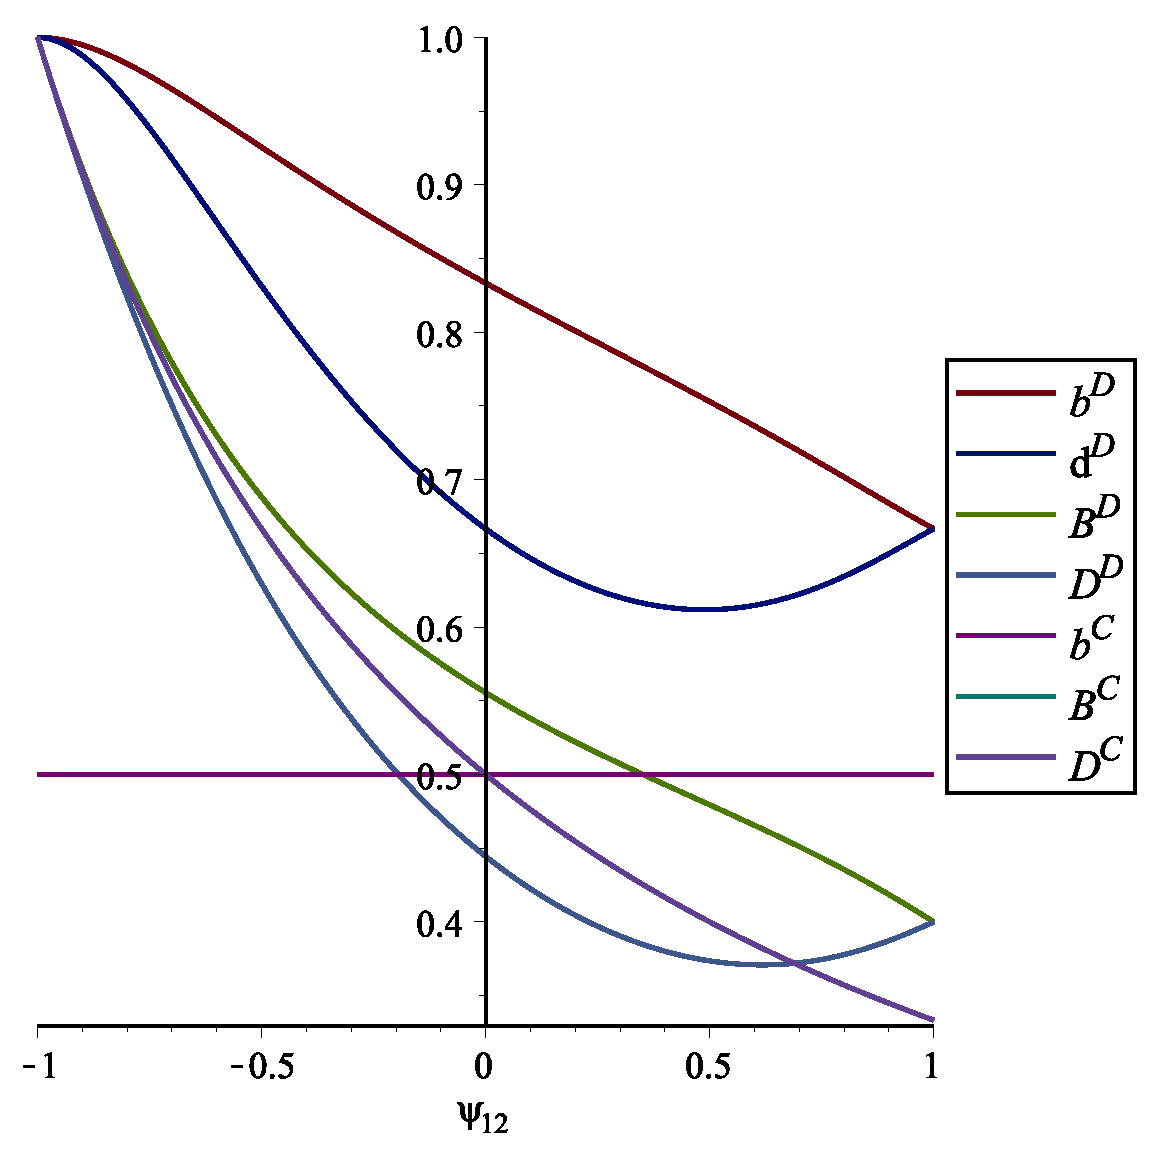
\includegraphics[width=0.65\textwidth]{gr1-eps-converted-to.pdf}
  \caption{Incentivos óptimos con estructuras descentralizada (D) y centralizada (C) para distintos valores de $\psi_{12}$}
  \label{fig:incentivos_psi}
\end{figure}

\begin{figure}[htbp]
  \centering
  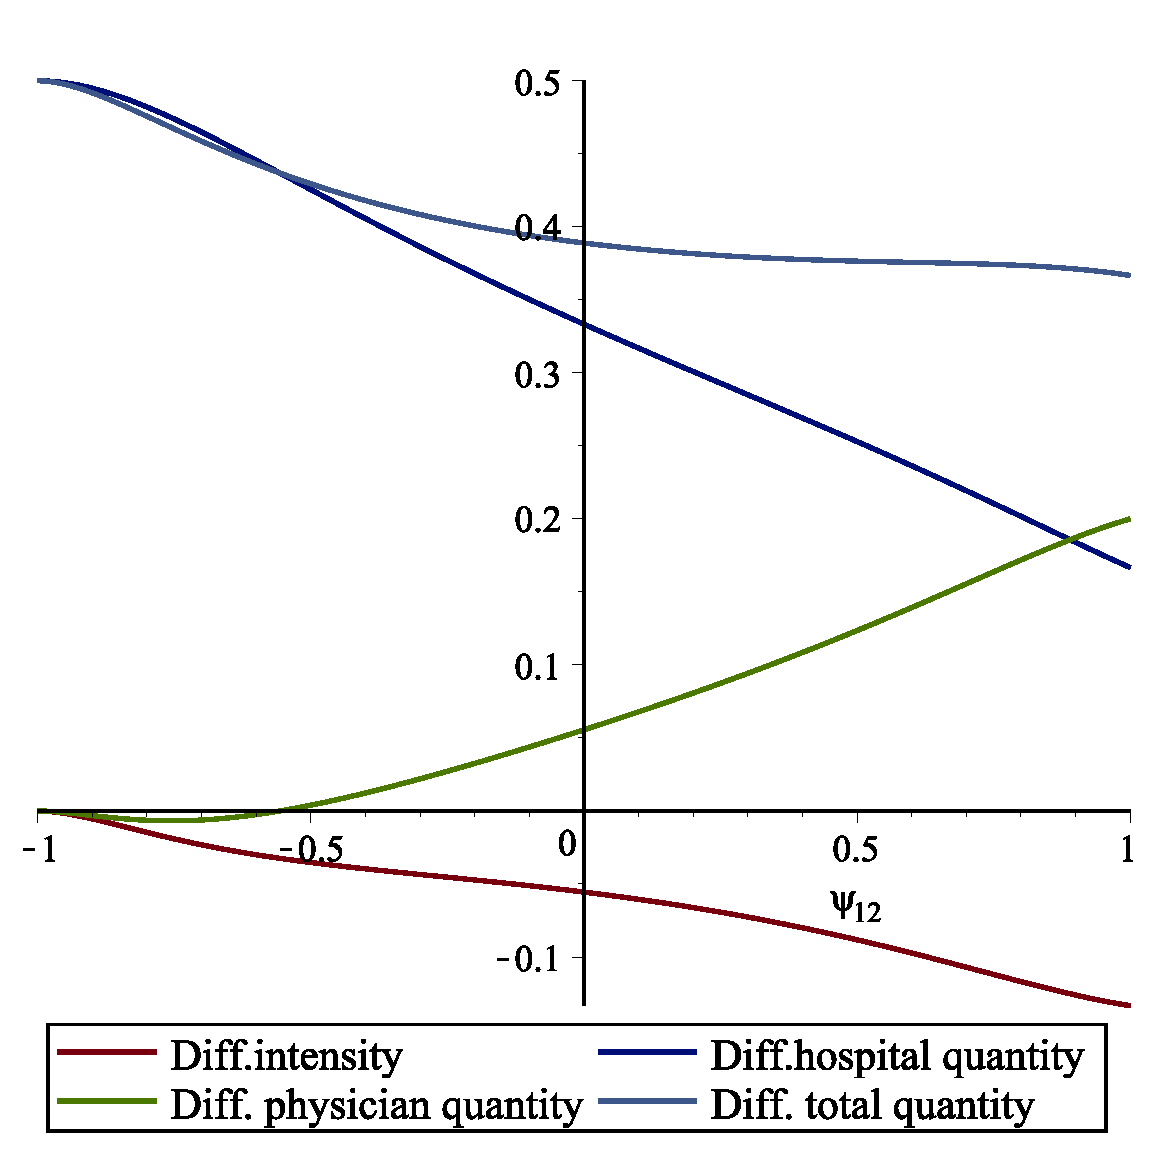
\includegraphics[width=0.65\textwidth]{gr2-eps-converted-to.pdf}
  \caption{Diferencial de esfuerzos (descentralizada frente a centralizada) para distintos valores de $\psi_{12}$}
  \label{fig:esfuerzos_psi}
\end{figure}

Los principales hallazgos respecto de la interacción entre tareas son:

\begin{result}[Efectos de $\psi_{12}$ sobre incentivos y esfuerzos]
\label{res:psi12}
\begin{enumerate}[label=(\alph*)]
  \item Los incentivos al hospital no dependen de $\psi_{12}$ en la estructura centralizada, pero sí en la descentralizada (\textit{potencia secuencialmente inducida}).
  \item Las estructuras descentralizadas crean un sesgo hacia la contratación de cantidad (excepto en sustitución perfecta).
  \item Bajo sustitución perfecta, la contratación centralizada óptima no implica incentivos para el médico (salarios fijos), mientras que los incentivos permanecen positivos y simétricos entre tareas en la descentralizada. \textit{La adecuación de los incentivos bajo riesgo moral depende del diseño organizativo vigente.}
  \item Cuando la cantidad se mide perfectamente ($\sigma_1=0$), ambas estructuras alcanzan niveles de primer \textit{best} en cantidad, mientras que la intensidad es mayor en la centralizada (Figura~\ref{fig:sigma1cero}).
  \item Cuando la intensidad se mide sin ruido ($\sigma_2=0$), ambas estructuras alcanzan primer \textit{best} en intensidad, pero la cantidad es mayor en la descentralizada (Figura~\ref{fig:sigma2cero}).
\end{enumerate}
\end{result}

\begin{figure}[htbp]
  \centering
  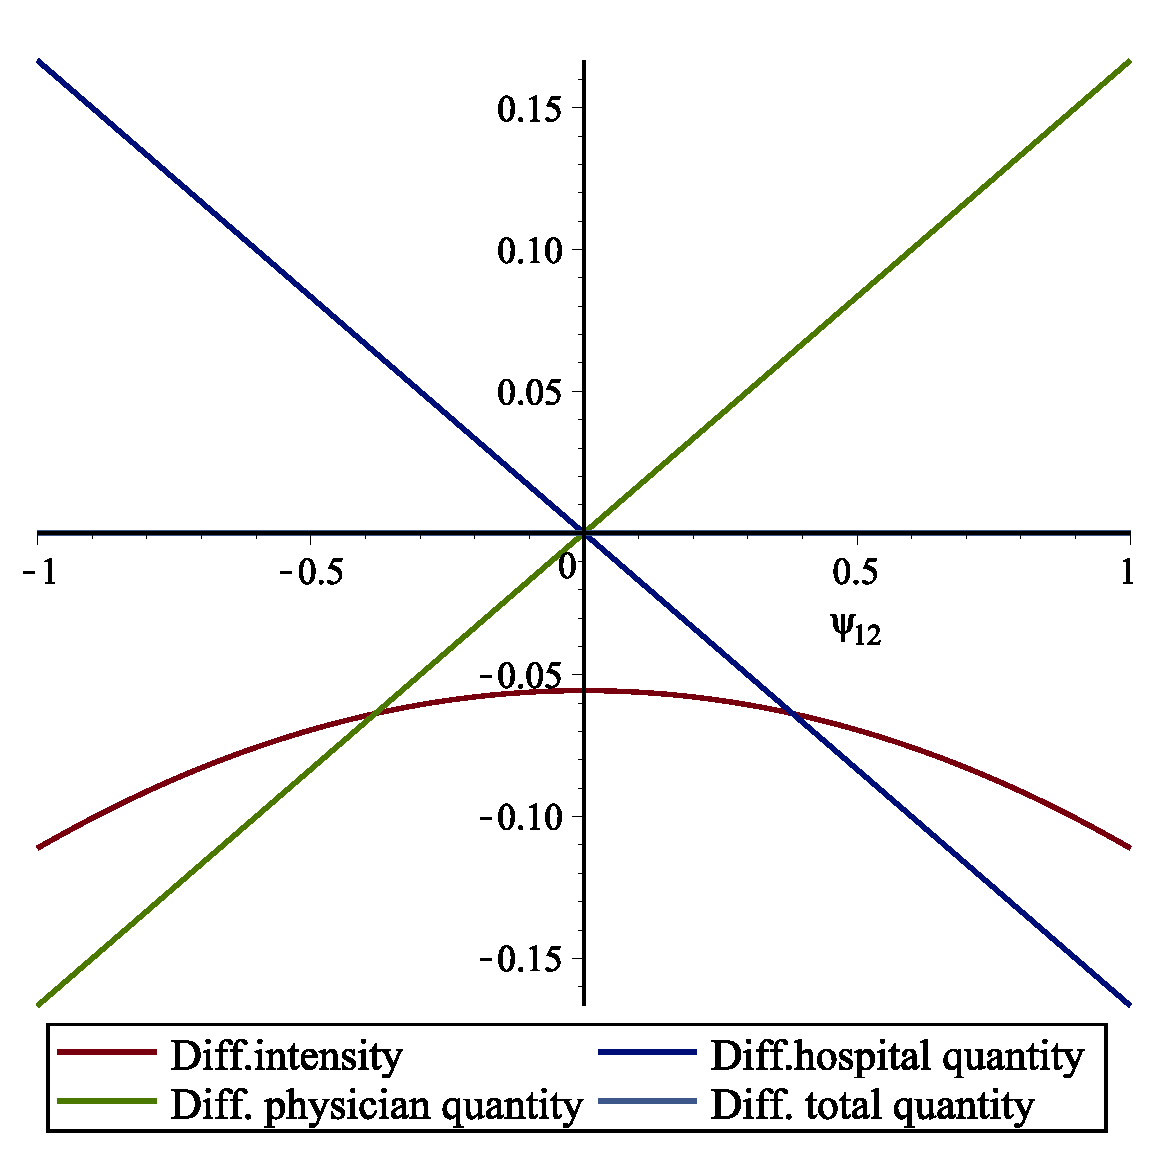
\includegraphics[width=0.65\textwidth]{gr3-eps-converted-to.pdf}
  \caption{Diferencial de esfuerzos dado $\sigma_1=0$}
  \label{fig:sigma1cero}
\end{figure}

\begin{figure}[htbp]
  \centering
  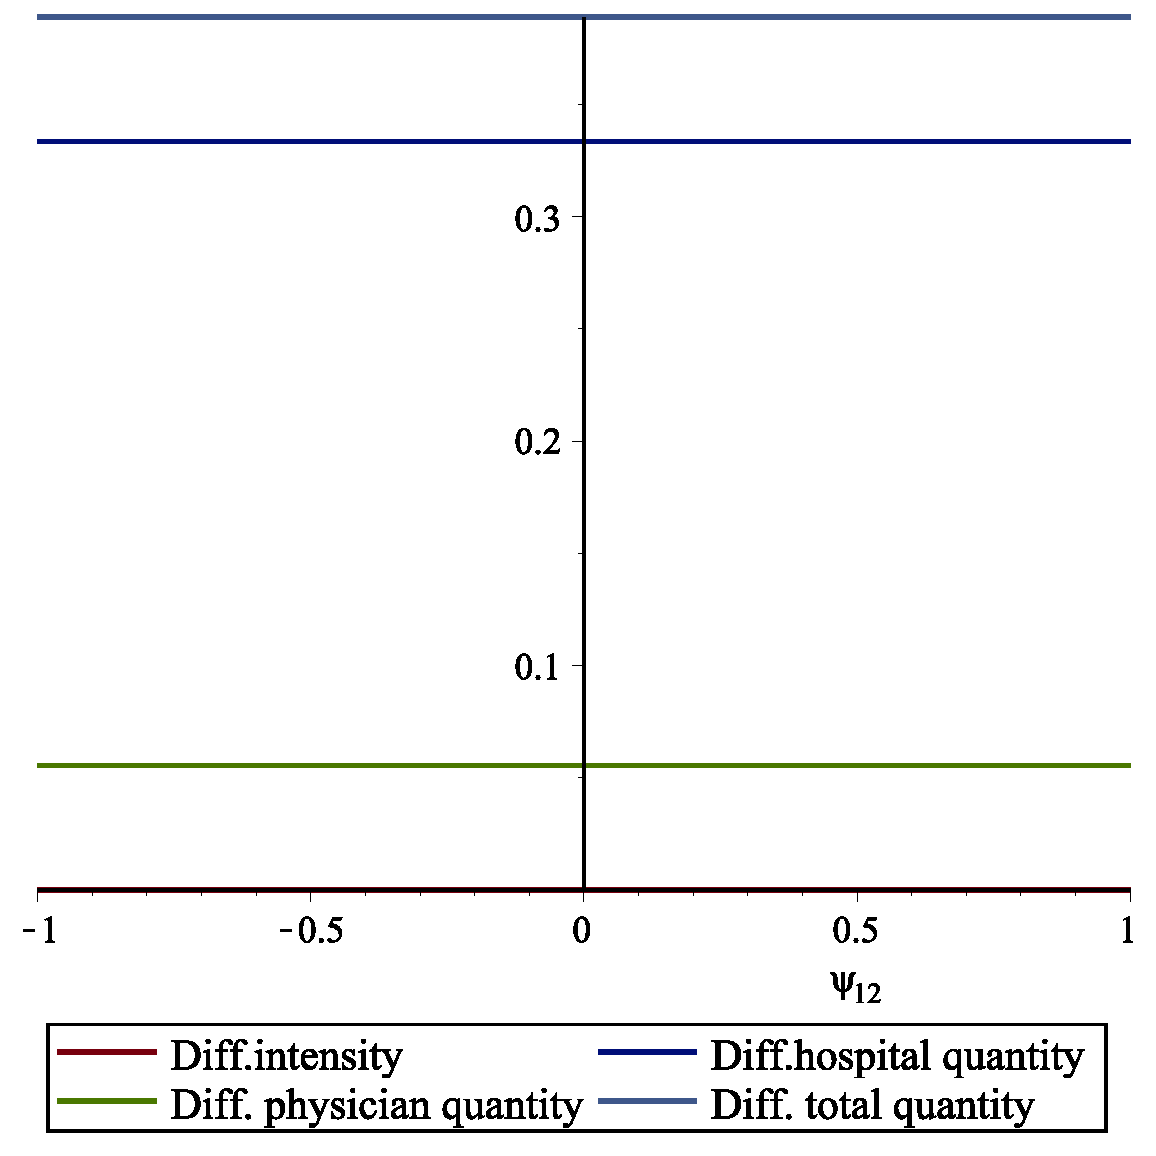
\includegraphics[width=0.65\textwidth]{gr4-eps-converted-to.pdf}
  \caption{Diferencial de esfuerzos dado $\sigma_2=0$}
  \label{fig:sigma2cero}
\end{figure}

\subsection{Medición imprecisa de los resultados}

Cuando la medición de la cantidad se vuelve más ruidosa (aumento de $\sigma_1$), para tareas sustitutivas ($\psi_{12}=0.5$):

\begin{figure}[htbp]
  \centering
  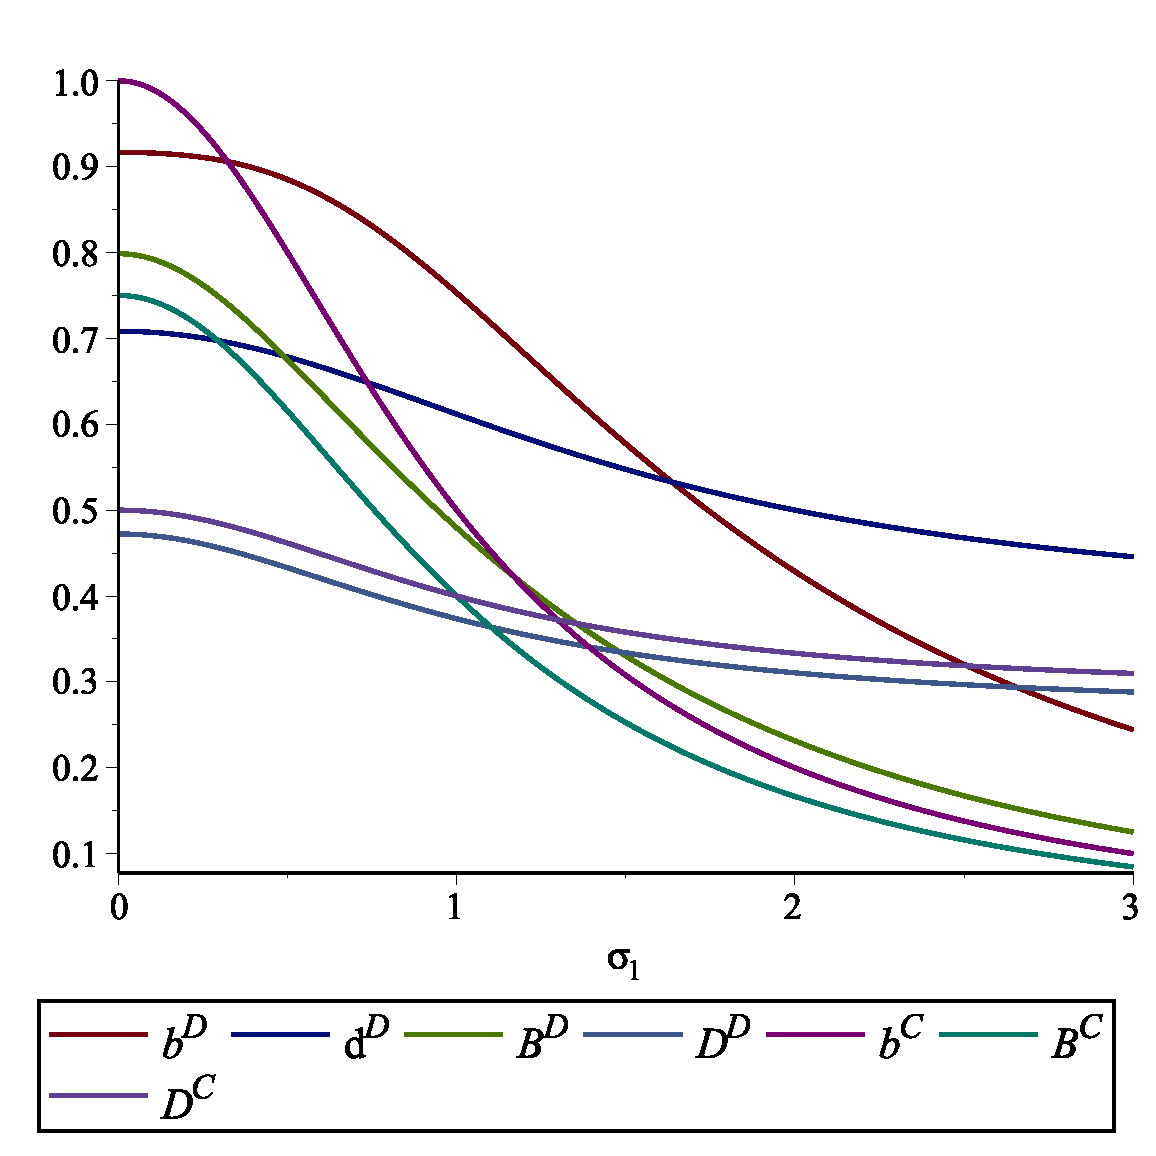
\includegraphics[width=0.65\textwidth]{gr5-eps-converted-to.pdf}
  \caption{Incentivos óptimos cuando aumenta $\sigma_1$}
  \label{fig:incentivos_sigma1}
\end{figure}

\begin{figure}[htbp]
  \centering
  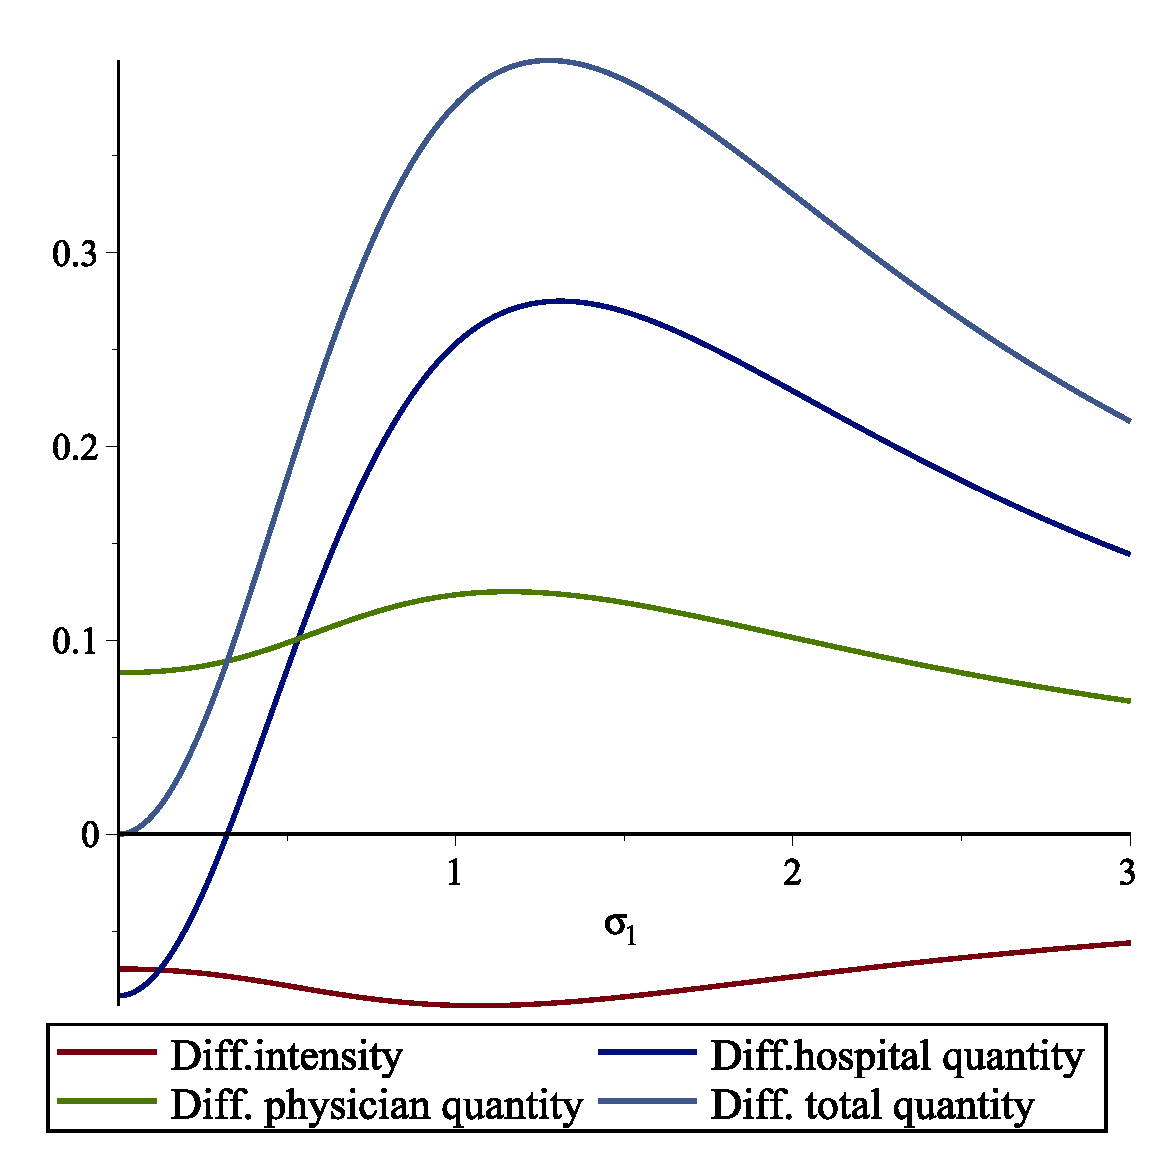
\includegraphics[width=0.65\textwidth]{gr6-eps-converted-to.pdf}
  \caption{Diferencial de esfuerzos cuando aumenta $\sigma_1$}
  \label{fig:esfuerzos_sigma1}
\end{figure}

\begin{result}[Efectos del ruido en la medición]
\label{res:ruido}
\begin{enumerate}[label=(\alph*)]
  \item Con ruido creciente en cantidad ($\sigma_1$): todos los incentivos disminuyen. Los pagos por cantidad tienden a cero; los de intensidad se estabilizan. La intensidad permanece mayor bajo centralización; la cantidad mayor bajo descentralización.
  \item Con ruido creciente en intensidad ($\sigma_2$) y tareas sustitutas (Figura~\ref{fig:esfuerzos_sigma2_sust}): la cantidad total permanece constante e independiente del ruido y es mayor en la descentralizada. La intensidad se reduce en la descentralizada respecto de la centralizada.
  \item Con ruido creciente en intensidad y tareas complementarias (Figura~\ref{fig:esfuerzos_sigma2_comp}): niveles bajos de $\sigma_2$ favorecen a la descentralizada incluso en intensidad. A medida que aumenta la imprecisión, los desempeños del médico pasan a favorecer la centralización, compensando la ventaja descentralizada en el esfuerzo hospitalario.
\end{enumerate}
\end{result}

\begin{figure}[htbp]
  \centering
  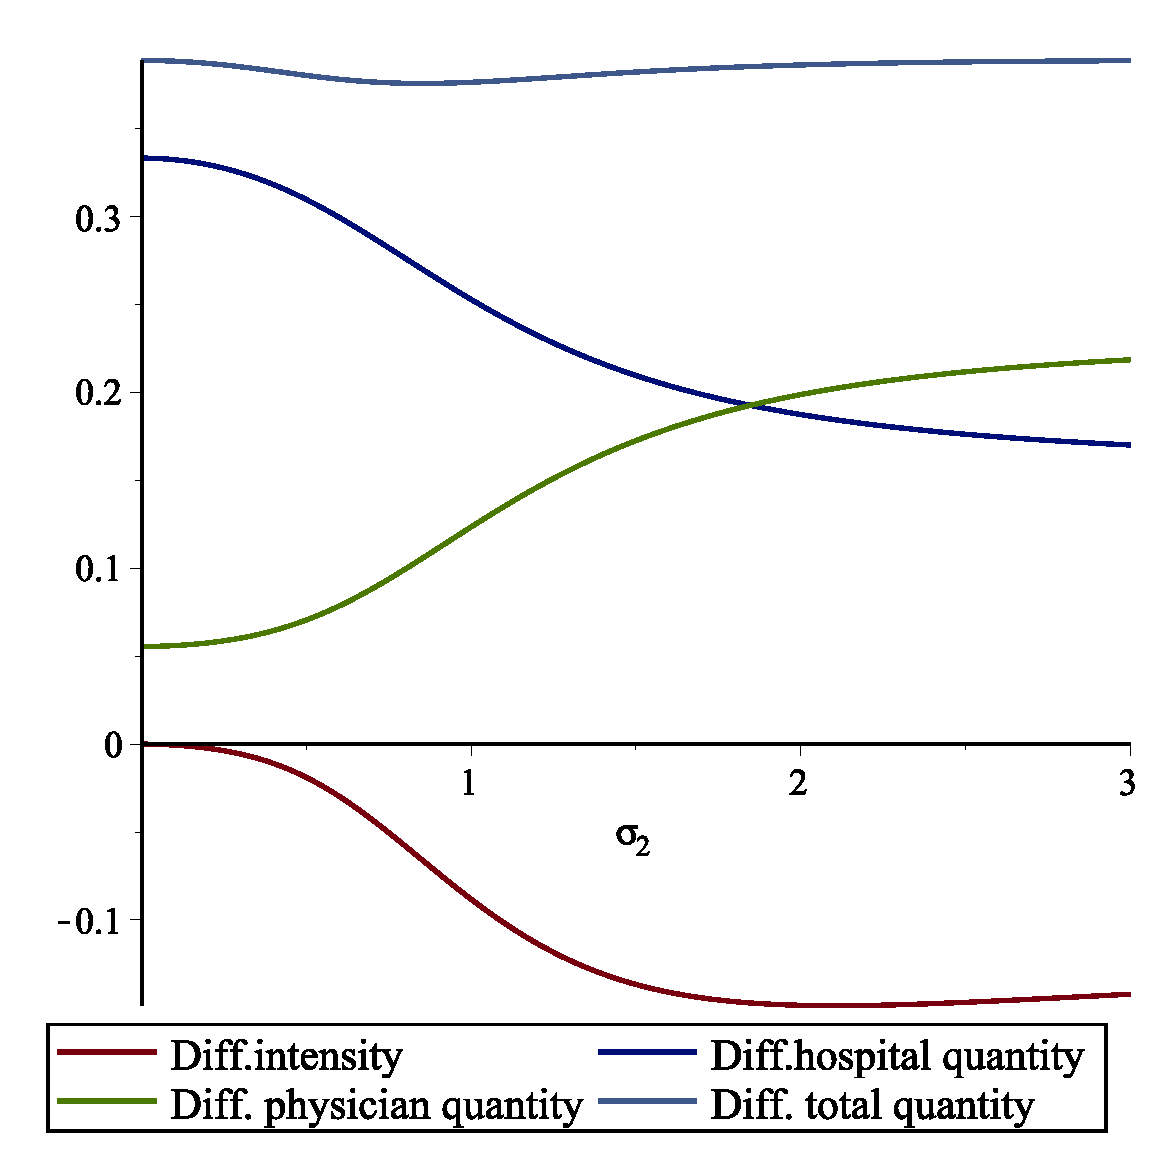
\includegraphics[width=0.65\textwidth]{gr8-eps-converted-to.pdf}
  \caption{Diferencial de esfuerzos cuando aumenta $\sigma_2$ (tareas sustitutas, $\psi_{12}=0.5$)}
  \label{fig:esfuerzos_sigma2_sust}
\end{figure}

\begin{figure}[htbp]
  \centering
  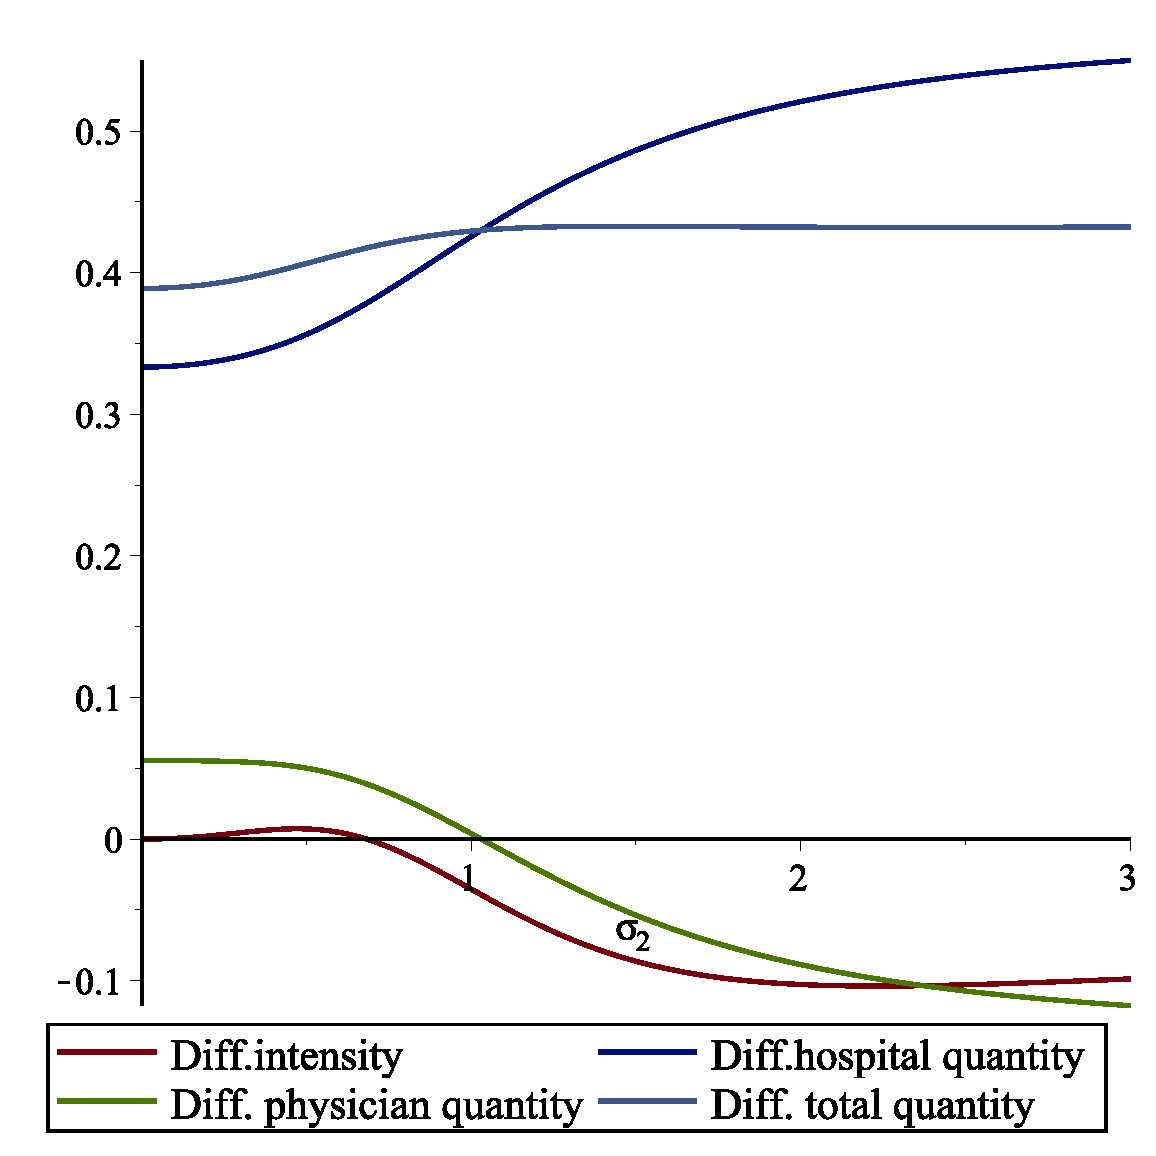
\includegraphics[width=0.65\textwidth]{gr9-eps-converted-to.pdf}
  \caption{Diferencial de esfuerzos cuando aumenta $\sigma_2$ (tareas complementarias, $\psi_{12}=-0.5$)}
  \label{fig:esfuerzos_sigma2_comp}
\end{figure}


\section{Predicciones contrastables}
\label{sec:predicciones}

Los resultados del modelo teórico pueden traducirse en hipótesis empíricamente contrastables sobre la eficiencia técnica hospitalaria. En el contexto del análisis de frontera estocástica, la ineficiencia técnica en cada dimensión del output se modeliza con media heterogénea que depende de la estructura organizativa, el mecanismo de pago y la interacción entre tareas.

\begin{table}[htbp]
\centering
\caption{Predicciones contrastables del modelo teórico}
\label{tab:predicciones}
\begin{threeparttable}
\begin{tabular}{clcc}
\toprule
\textbf{Pred.} & \textbf{Descripción} &
\textbf{Parámetro} & \textbf{Signo esperado} \\
\midrule
P1 & Descentralización $\downarrow$ ineficiencia en $q$
   & $\alpha_1$ en $\mu^q_{it}$ & $\alpha_1 < 0$ \\[3pt]
P2 & Descentralización $\uparrow$ ineficiencia en $i$
   & $\delta_1$ en $\mu^i_{it}$ & $\delta_1 > 0$ \\[3pt]
P3 & El tipo de pago difiere entre dimensiones
   & $\alpha_2 \neq \delta_2$ & Signos opuestos \\[3pt]
P4 & $\psi_{12}$ modera asimétricamente el diferencial
   & $\alpha_4 \neq \delta_4$ & Signos opuestos \\[3pt]
P$^*$ & El vector de determinantes difiere entre
         dimensiones & $\bsym{\alpha} \neq \bsym{\delta}$
       & Rechazado \\
\bottomrule
\end{tabular}
\begin{tablenotes}
  \small
  \item Nota: $\mu^q_{it}$ y $\mu^i_{it}$ son las medias heterogéneas de los términos de ineficiencia en las fronteras de cantidad e intensidad. $\bsym{\alpha}$ y $\bsym{\delta}$ son los vectores completos de coeficientes de la ecuación de ineficiencia en cada frontera.
\end{tablenotes}
\end{threeparttable}
\end{table}

La predicción P1 se fundamenta en el Resultado~\ref{res:comparacion_independientes}(a): la estructura descentralizada induce mayor esfuerzo hospitalario en cantidad. La predicción P2 se fundamenta en el Resultado~\ref{res:comparacion_independientes}(b): ese mismo mecanismo reduce el esfuerzo médico en intensidad cuando las tareas son sustitutas. Las predicciones P3 y P4 capturan, respectivamente, la interacción del mecanismo de pago y del parámetro $\psi_{12}$ con la estructura organizativa.

\begin{remark}[Necesidad de dos términos de ineficiencia]
Si los efectos de P1 y P2 son de signo contrario, un modelo con un único término de ineficiencia $u_{it}$ cancela algebraicamente ambos efectos: la descentralización mejoraría la eficiencia en una dimensión y la empeoraría en otra, pero la ineficiencia agregada podría no cambiar. Ningún contraste directamente relevante para el modelo teórico es identificable con un único $u_{it}$. Esta observación motiva el uso de un sistema de dos fronteras estocásticas.
\end{remark}


\section{Discusión y conexión con la literatura}
\label{sec:discusion_literatura}

Los resultados derivados en las secciones anteriores guardan una relación estrecha con varios cuerpos de literatura, pero también se apartan en aspectos importantes que conviene destacar.

\subsection{Relación con Holmström-Milgrom (1991)}

El modelo seminal de \citet{holmstrom1991} establece que, cuando un agente realiza múltiples tareas y el principal solo puede incentivar algunas de ellas, los incentivos sobre las tareas medibles pueden distorsionar el esfuerzo en detrimento de las tareas no medibles. En nuestro modelo, este mecanismo se activa en la relación hospital-médico: cuando el hospital incentiva al médico sobre la dimensión de cantidad (medible y verificable mediante altas), el médico puede desplazar esfuerzo desde la dimensión de intensidad (más difícil de verificar). El resultado de \citet{holmstrom1991} en nuestro contexto se aplica tanto en la estructura centralizada como en la descentralizada, pero con intensidades distintas: en la descentralizada, el hospital internaliza el efecto de sustitución al diseñar el contrato del médico, lo que modifica la potencia óptima de los incentivos respecto del caso centralizado.

La diferencia fundamental respecto de \citet{holmstrom1991} es la presencia de tres agentes. En su modelo hay un único principal y un único agente con múltiples tareas. En nuestro modelo, el principal interactúa con el hospital, que a su vez interactúa con el médico. Esta estructura de jerarquía crea una cadena de incentivos en que el primer nivel condiciona el segundo. El resultado de que los incentivos del hospital dependan de $\psi_{12}$ en la estructura descentralizada ---pero no en la centralizada--- es una consecuencia directa de esta jerarquía que no tiene análogo en el modelo bilateral de \citet{holmstrom1991}.

\subsection{Relación con Jelovac-Macho-Stadler (2002)}

\citet{jelovac2002} estudian el diseño óptimo de contratos en un sistema de salud con un pagador, un hospital y un médico, analizando cuándo es óptima la contratación centralizada versus la descentralizada. Su modelo distingue, como el nuestro, entre un hospital que gestiona la cantidad de servicios y un médico que determina la calidad (o intensidad). El resultado central de \citet{jelovac2002} es que la estructura organizativa óptima depende de las características del médico (altruismo, aversión al riesgo) y del tipo de servicio (preventivo vs. curativo).

Nuestro modelo se aparta de \citet{jelovac2002} en varios aspectos relevantes. \textit{Primero}, explicitamos la función de costes del médico con el parámetro de sustitución $\psi_{12}$, que \citet{jelovac2002} no incluyen. \textit{Segundo}, mientras que \citet{jelovac2002} resuelven el problema de elección del diseño organizativo óptimo (¿cuándo debe el financiador centralizar o descentralizar?), nuestro objetivo es caracterizar las diferencias en los resultados bajo ambas estructuras dadas (no la elección óptima entre ellas). \textit{Tercero}, nuestro modelo permite simulaciones numéricas que cubren el espacio de parámetros completo, más allá de las condiciones analíticas disponibles en forma cerrada.

\subsection{Relación con Eggleston (2005)}

\citet{eggleston2005} examina los efectos de distintos mecanismos de pago sobre la provisión de calidad en un modelo de multitarea hospitalaria. Su resultado central es que un aumento en el poder del pago por actividad (pago prospectivo) puede deteriorar la calidad si las tareas son sustitutas en la función de costes del médico. Este resultado es coherente con nuestras predicciones P1 y P2: la descentralización, que en nuestro modelo va acompañada de mayor uso de pago por actividad (menor $pct^{SNS}$), reduce la ineficiencia en cantidad pero puede no mejorar la intensidad de forma proporcional.

La diferencia principal es que \citet{eggleston2005} trabaja con un modelo de un solo nivel (pagador-médico), sin la jerarquía hospital-médico. Nuestra aportación es mostrar que la transmisión de incentivos a través de la jerarquía hospital-médico modifica los resultados de forma no trivial: incluso bajo estructura descentralizada, el hospital tiene incentivos para internalizar la sustitución de esfuerzo del médico, lo que puede atenuar el deterioro de la intensidad respecto de lo predicho por un modelo de un solo nivel.

\subsection{Relación con Kaarboe-Siciliani (2011)}

\citet{kaarboe2011} estudian los incentivos del médico hospitalario en un modelo de multitarea (cantidad versus calidad) con información asimétrica. Su resultado de \textit{multitasking penalty} ---la pérdida de bienestar asociada a la imposibilidad de incentivar simultáneamente ambas dimensiones del output--- tiene un paralelo directo en nuestro modelo: la imposibilidad de medir la intensidad con precisión ($\sigma_2$ elevado) reduce la potencia óptima de los incentivos sobre esa dimensión.

Nuestra extensión respecto de \citet{kaarboe2011} reside en la distinción entre estructuras organizativas: el \textit{multitasking penalty} tiene una magnitud distinta en la estructura centralizada y en la descentralizada, y depende crucialmente del signo de $\psi_{12}$. Esta interacción entre estructura organizativa, tipo de pago y complementariedad entre tareas es la contribución central de nuestro modelo a la literatura.

\section{Conclusiones del modelo teórico}
\label{sec:conclusiones_modelo}

En las páginas anteriores hemos caracterizado los rasgos principales de un modelo de provisión sanitaria en una configuración de múltiples agentes y múltiples outputs. El propósito ha sido obtener resultados relevantes sobre la potencia óptima de los incentivos y los esfuerzos ejercidos por los agentes bajo riesgo moral.

En un caso de referencia con información simétrica, el principal utiliza pagos de suma fija y mantiene a los agentes en sus utilidades de reserva. No se incluyen incentivos en el contrato óptimo. Hospital y médico igualan costes marginales en la producción de cantidad, y la tasa marginal de sustitución entre outputs iguala la tasa marginal de transformación entre tareas. Una implicación directa es la relación entre el altruismo del agente y el nivel de esfuerzo requerido: si el hospital tiene un componente vocacional mayor (propio de hospitales públicos o sin ánimo de lucro), el principal debería exigirle un nivel de esfuerzo mayor, pues puede explotar el beneficio que el agente obtiene de su componente altruista. Del mismo modo, si el único agente con preocupación directa por el bienestar del paciente es el médico, el principal contratará un mayor nivel de esfuerzo en intensidad relativa a la cantidad, comparado con el caso de un hospital con componente altruista.

Bajo acciones ocultas, la principal conclusión es que la estructura organizativa interactúa de formas complejas con la potencia óptima de los incentivos. Los resultados principales pueden resumirse así:

\begin{enumerate}[label=(\roman*)]
  \item En la estructura centralizada, los incentivos son independientes entre agentes: cambiar los incentivos del hospital no afecta a los del médico. En la descentralizada, están conectados por construcción, porque el hospital internaliza el problema de sustitución de esfuerzo del médico al diseñar su propio contrato con el principal. A este fenómeno puede llamársele \textit{potencia secuencialmente inducida de los incentivos}.

  \item Tanto en estructuras centralizadas como descentralizadas, la potencia óptima de los incentivos no depende del componente altruista o vocacional de los agentes. Bajo información asimétrica, el esquema óptimo de pagos es el mismo independientemente de si el hospital o el médico tienen motivación vocacional.

  \item La \textit{complementariedad de incentivos} ---que los pagos variables sobre las dos tareas del médico deban moverse en la misma dirección, resultado general de la literatura \citep[p.\ 222]{bolton2005}--- se matiza en nuestro modelo: bajo estructura centralizada, solo se aplica al contrato del médico (los incentivos de hospital y médico son independientes), mientras que bajo estructura descentralizada la complementariedad de incentivos alcanza también al hospital porque el hospital ya ha internalizado el problema de sustitución de esfuerzo.

  \item Bajo riesgo moral y pago fijo sin incentivos, el nivel de esfuerzo del hospital será inferior al de segundo \textit{best}. El esfuerzo del médico dependerá de sus parámetros: dado que $\psi_1=\psi_2$ y $\sigma_2>\sigma_1$, el esfuerzo en intensidad será mayor y el esfuerzo en cantidad menor que en el óptimo. Los pagos fijos generan una cantidad por debajo de la óptima y una intensidad por encima de la óptima: hay \textit{subprovisión de cantidad y sobreprovisión de intensidad}.

  \item Bajo un esquema que solo proporcione incentivos sobre cantidad ($b=b^C$, $B=B^C$, $D=0$), tanto hospital como médico proporcionan mayor esfuerzo en cantidad, pero el médico \textit{infraofrece} esfuerzo en intensidad. Este es el mecanismo de sustitución de esfuerzo predicho por \citet{holmstrom1991} en el contexto hospitalario.

  \item Bajo un esquema mixto en el que el hospital recibe incentivos óptimos pero el médico no ($b=b^C$, $B=D=0$), dependiendo de los valores de los parámetros, puede observarse \textit{infraprovisión tanto de cantidad como de intensidad}.

  \item En general, la intensidad es mayor en las estructuras centralizadas y la cantidad total en las descentralizadas: $a^D>a^C$ y $t_2^D<t_2^C$. Este es el resultado clave de la comparación entre estructuras para tareas independientes. La condición para que el esfuerzo del médico en cantidad sea mayor bajo centralización es $\eta\tau\sigma_1^2>1+\sigma_1^2\theta\psi_1$: cuando el coste marginal de producir cantidad por parte del hospital es suficientemente mayor que el del médico, la centralización domina incluso en cantidad.

  \item Bajo sustitución perfecta, la estructura centralizada óptima no implica incentivos para el médico (salarios fijos), mientras que la descentralizada mantiene incentivos positivos y simétricos entre tareas. Este resultado vincula estructura organizativa y tipo de contrato médico de forma directa y ayuda a comprender por qué los hospitales privados con mayor autonomía utilizan con mayor frecuencia esquemas de retribución variable para los médicos.

  \item Las estructuras descentralizadas crean un sesgo hacia la contratación de cantidad (excepto bajo sustitución perfecta): la potencia de los incentivos sobre cantidad en la descentralizada es mayor que sobre intensidad para la mayor parte del espacio de parámetros.

  \item La fuente de la asimetría de información tiene una recomendación distinta en términos de diseño organizativo dependiendo de si las tareas son sustitutas o complementarias. Cuando las tareas son complementarias, niveles bajos de ruido en intensidad favorecen incluso a la descentralización tanto en cantidad como en intensidad. A medida que aumenta la imprecisión en la medición de la intensidad, la centralización pasa a dominar también en intensidad.

  \item Cuando la cantidad se mide sin ruido ($\sigma_1=0$), ambas estructuras alcanzan niveles de primer \textit{best} en cantidad, mientras que la intensidad permanece mayor bajo centralización. Cuando la intensidad se mide sin ruido ($\sigma_2=0$), ambas estructuras alcanzan primer \textit{best} en intensidad, pero la cantidad es mayor bajo descentralización. Estas asimetrías sugieren que el diseño organizativo óptimo depende de cuál es la dimensión del output con mayor incertidumbre de medición.
\end{enumerate}

\begin{remark}[Implicaciones de mecanismo]
La cadena de causalidad del modelo puede describirse del siguiente modo. La descentralización amplía la autonomía del hospital para diseñar el contrato médico. El hospital, que recibe incentivos sobre la cantidad ($b$ en el pago del principal), tiene incentivos para maximizar el esfuerzo del médico en cantidad ($B$ elevado). Bajo sustitución de tareas ($\psi_{12}>0$), esto desplaza esfuerzo desde la intensidad. En la centralizada, el principal diseña directamente el contrato del médico sin pasar por la maximización del hospital, lo que permite equilibrar los incentivos sobre ambas tareas. Este mecanismo es el fundamento teórico de las predicciones P1 y P2.
\end{remark}

Estos resultados teóricos se traducen en las predicciones contrastables P1--P$^*$ de la Tabla~\ref{tab:predicciones}, que serán el objeto del análisis empírico en los capítulos siguientes.

En suma, bajo riesgo moral y múltiples outputs, la estructura organizativa interactúa de formas complejas con la potencia óptima de los incentivos que debe utilizarse. El resultado general de que la intensidad es mayor en las estructuras centralizadas y la cantidad total en las descentralizadas debe matizarse dependiendo de la interacción tecnológica entre tareas ($\psi_{12}$) y del grado de incertidumbre en la medición de cada dimensión del output ($\sigma_1$ y $\sigma_2$). La aplicación empírica de estas predicciones mediante análisis de frontera estocástica con datos del sistema hospitalario español constituye el objeto de los capítulos siguientes.



% ###########################################################
% CAPÍTULO 3: ESTRATEGIA EMPÍRICA
% ###########################################################
\chapter{Estrategia empírica}
\label{ch:estrategia}

\section{Motivación empírica}

Este capítulo desarrolla la estrategia empírica para contrastar las predicciones del modelo teórico del Capítulo~\ref{ch:modelo}. La contribución empírica central es identificar y contrastar la asimetría predicha utilizando un sistema de fronteras estocásticas con datos de panel del sistema hospitalario español para el período 2010--2023. La evidencia producida es, hasta donde conocemos, la primera contrastación empírica directa de un modelo de agencia multitarea en el sector hospitalario español mediante análisis de frontera estocástica.

\section{Marco general: análisis de frontera estocástica}

El análisis de frontera estocástica (SFA), desarrollado simultáneamente por \citet{aigner1977} y \citet{meeusen1977}, descompone la desviación de un hospital respecto a la frontera de producción en dos componentes:
\begin{equation}
  \ln y_{it} = f(\mathbf{x}_{it};\,\bsym{\beta}) + v_{it} - u_{it}
  \label{eq:sfa_base}
\end{equation}
donde $v_{it} \sim \N(0, \sigma^2_v)$ es ruido aleatorio simétrico y $u_{it} \geq 0$ es el término de ineficiencia técnica. La eficiencia técnica del hospital $i$ en el período $t$ se estima como:
\begin{equation}
  TE_{it} = \E\!\left[e^{-u_{it}} \mid \varepsilon_{it}\right]
  \label{eq:te}
\end{equation}
siguiendo el estimador de \citet{jondrow1982}.

Para incorporar los determinantes de la ineficiencia, se adopta la especificación de \citet{battese1995}, donde $u_{it}$ sigue una distribución normal truncada en cero con media heterogénea:
\begin{equation}
  u_{it} \sim \N^+\!\left(\mu_{it},\, \sigma^2_u\right), \quad \mu_{it} = \mathbf{z}_{it}'\bsym{\delta}
  \label{eq:bc95}
\end{equation}
Esta especificación, extendida por \citet{wang2002} para permitir heterogeneidad también en la varianza de $u_{it}$, es la base de todos los diseños de estimación. El SFA se ha aplicado extensamente al sector hospitalario, incluyendo los trabajos de \citet{puigjunoy2000} para España, \citet{linna1998} para Finlandia, \citet{rosko2008} para Estados Unidos y \citet{street2003} para el NHS británico.

\section{Especificación de la frontera de producción}

Para todos los diseños se adopta una forma funcional translog en los inputs, centrada en las medias muestrales para facilitar la interpretación:
\begin{align}
  \ln y_{kit} &= \beta_0
    + \beta_1 \ln\tilde{L}_{it}
    + \beta_2 \ln\tilde{K}^C_{it}
    + \beta_3 \ln\tilde{K}^T_{it}
    + \beta_4 (\ln\tilde{L}_{it})^2
    + \beta_5 (\ln\tilde{K}^C_{it})^2
    \notag \\
    &\quad
    + \beta_6\, t
    + \beta_7\, t^2
    + \sum_{g=2}^{5} \gamma_g\, D^{cluster}_g
    + v_{it} - u_{kit}
  \label{eq:frontera_tl}
\end{align}
donde $\tilde{L}_{it}$, $\tilde{K}^C_{it}$ y $\tilde{K}^T_{it}$ son los logaritmos centrados del personal médico EJC, las camas en funcionamiento y el índice tecnológico. La tendencia temporal $t$ captura el progreso técnico. Las dummies $D^{cluster}_g$ controlan la heterogeneidad tecnológica entre grupos de hospitales de distinta complejidad, siguiendo la clasificación del Ministerio de Sanidad \citep{ministerio2007}.\footnote{El término de interacción $\ln\tilde{L}\times\ln\tilde{K}^C$ se eliminó de la especificación por multicolinealidad severa ($r=0.953$ con $(\ln\tilde{L})^2$). El \textit{condition number} de la matriz translog reducida es 171, manejable. La translog es estadísticamente preferida sobre Cobb-Douglas mediante tests LR con estadísticos entre 246 y 594 ($p<0.001$).}

\section{Ecuación de ineficiencia}
\label{sec:ecuacion_inef}

La media heterogénea del término de ineficiencia es:
\begin{align}
  \mu_{kit} &= \delta_0
    + \delta_1\, D^{desc}_{it}
    + \delta_2\, pct^{SNS}_{it}
    + \delta_3\, (D^{desc}_{it} \times pct^{SNS}_{it})
    + \delta_4\, ShareQ_{it}
    + \delta_5\, (D^{desc}_{it} \times ShareQ_{it})
    \notag \\
    &\quad + \sum_{c \neq 9} \lambda_c\, D^{ccaa}_{c,it}
    + \omega_{kit}
  \label{eq:uhet}
\end{align}
donde $D^{desc}_{it}$ es la variable de estructura organizativa (1 = descentralizado, 0 = centralizado SNS), $pct^{SNS}_{it}$ es la proporción de altas financiadas por el SNS como proxy del mecanismo de pago, $ShareQ_{it}$ es la proporción de altas quirúrgicas sobre el total como proxy de $\psi_{12}$, y $D^{ccaa}_{c,it}$ son dummies de comunidad autónoma que absorben la heterogeneidad regional (referencia: Cataluña, $c=9$).

Cada variable de la ecuación de ineficiencia tiene un anclaje directo en el modelo teórico:
\begin{itemize}
  \item $D^{desc}$: capta el efecto de la estructura organizativa (centralizada vs.\ descentralizada) sobre la ineficiencia. Sus coeficientes en las dos fronteras son los parámetros $\alpha_1$ y $\delta_1$ de las predicciones P1 y P2.
  \item $pct^{SNS}$: aproxima el mecanismo de pago. Un hospital con alta proporción de altas SNS está sujeto predominantemente a financiación prospectiva por actividad o presupuesto global.
  \item $D^{desc}\times pct^{SNS}$: captura la interacción entre estructura y tipo de pago (predicción P3).
  \item $ShareQ$: proxy continua de $\psi_{12}$. Hospitales con alta proporción de actividad quirúrgica operan en un régimen de complementariedad entre tareas.
  \item $D^{desc}\times ShareQ$: moderación de $\psi_{12}$ sobre el efecto de la descentralización (predicción P4).
\end{itemize}

\section{Los cuatro diseños de estimación}

Se plantean cuatro diseños complementarios con roles distintos en la estructura del análisis (Tabla~\ref{tab:disenos}).

\begin{table}[htbp]
\centering
\caption{Diseños de estimación y su papel en el análisis}
\label{tab:disenos}
\begin{threeparttable}
\small
\begin{tabular}{p{1.2cm}p{3.5cm}p{2.5cm}p{3.5cm}}
\toprule
\textbf{Diseño} & \textbf{Descripción} &
\textbf{Permite} & \textbf{Papel} \\
\midrule
D & Función de distancia output (ODF) con dos outputs simultáneos y un único $u_{it}$
  & P3, P4 (no P1/P2)
  & Punto de partida metodológico \\[6pt]
A & Sistema de dos fronteras: cantidad total e intensidad diagnóstica
  & P1, P2, P3, P4, P$^*$
  & Contraste directo del modelo teórico \\[6pt]
B & Sistema de dos fronteras: altas quirúrgicas y altas médicas
  & P1, P3, P4, P$^*$
  & Contraste con proxy estructural de $\psi_{12}$ \\[6pt]
C & Panel hospital $\times$ servicio $\times$ año
  & P4 con variación intra-hospital
  & Robustez con variación dentro del hospital \\
\bottomrule
\end{tabular}
\end{threeparttable}
\end{table}

\subsection{Diseño D --- Función de distancia output}

Siguiendo a \citet{coelli1999}, se estima una función de distancia output translog con dos outputs (altas quirúrgicas y médicas ponderadas). La normalización por el output quirúrgico impone homogeneidad de grado 1 en outputs:
\begin{equation}
  -\ln altQ^{pond}_{it} = f\!\left(\frac{altM^{pond}_{it}}{altQ^{pond}_{it}},\, \mathbf{x}_{it}\right) + v_{it} - u_{it}
  \label{eq:odf}
\end{equation}

El Diseño D no puede falsificar P1 ni P2 porque dispone de un único $u_{it}$: los efectos de signo contrario de la descentralización sobre las dos dimensiones se cancelan. Sirve para P3 y P4 y para analizar la distribución interna de la ineficiencia entre outputs, y proporciona un punto de partida metodológico que establece la existencia de ineficiencia significativa \citep{coelli2005}.

\subsection{Diseño A --- Sistema bivariado cantidad/intensidad}

Es el diseño más cercano al modelo teórico. Estima dos fronteras independientes, una para la cantidad total ($\ln altTotal^{pond}$) y otra para la intensidad ($\ln i_{diag}$), con ecuaciones de ineficiencia que comparten las mismas variables explicativas. El contraste central es:
\begin{equation}
  H_0:\; \bsym{\alpha} = \bsym{\delta}
  \label{eq:h0_pstar}
\end{equation}

La variable de intensidad $i_{diag}$ se construye como un índice ponderado de procedimientos diagnósticos por alta:
\begin{equation}
  i_{diag,it} = \frac{\sum_p w_p \cdot n_{p,it}}{altTotal^{pond}_{it}}
  \label{eq:i_diag}
\end{equation}
donde $w_p$ es el peso relativo de cada tipo de procedimiento (TAC, RNM, PET, angiografía, gammagrafía, colonoscopia, etc.) y $n_{p,it}$ es el número de procedimientos realizados. Los datos proceden del módulo C1\_16 del SIAE.\footnote{En 2021 el módulo C1\_16 cambió la denominación de variables de procedimientos. Se verificó la coherencia de la serie temporal: la mediana de $i_{diag}$ se mantiene estable en el rango 8.1--9.5 durante 2010--2023.}

\subsection{Diseño B --- Sistema bivariado quirúrgico/médico}

En lugar de medir $i$ directamente, redefine los dos outputs usando la desagregación del SIAE por tipo de servicio. La justificación estructural es directa desde el modelo teórico: los servicios quirúrgicos son el caso canónico de $\psi_{12} < 0$ (complementariedad), porque el acto quirúrgico implica per se alta intensidad; los servicios médicos son el caso de $\psi_{12} > 0$ (sustitución), porque ver más pacientes compite con el tiempo diagnóstico por paciente.

La ventaja operacional es que elimina la necesidad de medir la intensidad directamente y utiliza una clasificación estructural como proxy de $\psi_{12}$.

\subsection{Diseño C --- Panel hospital \texorpdfstring{$\times$}{x} servicio}

Construye un panel largo con dos filas por hospital-año (quirúrgicos y médicos) y estima una frontera única con la interacción $D^{desc}\times C_s$ en la ecuación de ineficiencia. El coeficiente captura si la descentralización afecta de forma diferente a los servicios quirúrgicos que a los médicos, con la ventaja de explotar variación \textit{dentro} del hospital.

\section{Estimación e inferencia}

Todos los modelos se estiman por máxima verosimilitud utilizando el paquete \texttt{sfaR} \citep{dakpo2024} en R. La secuencia de optimización intenta sucesivamente los métodos BFGS, BHHH y Nelder-Mead con distribuciones normal truncada (\texttt{tnormal}) y seminormal (\texttt{hnormal}).\footnote{Una solución se considera degenerada si la log-verosimilitud no es finita, si algún coeficiente supera 100 en valor absoluto, o si algún error estándar de los coeficientes de ineficiencia no es finito.}

Para el test conjunto P$^*$ se utiliza un test de razón de verosimilitud (LR):
\begin{equation}
  LR = 2\left(\ell^{irr} - \ell^{restr}\right) \sim \chi^2(k)
  \label{eq:lr_test}
\end{equation}
donde $\ell^{irr}$ es la suma de log-verosimilitudes de los modelos separados y $\ell^{restr}$ corresponde al modelo con muestras apiladas e igualdad de coeficientes.\footnote{Se intentó un bootstrap paramétrico con $B=4{,}999$ réplicas, pero la tasa de convergencia fue del 2.9\% en el Diseño A y del 0.06\% en el Diseño B, insuficiente para construir una distribución empírica fiable. La baja convergencia se debe a la concentración geográfica de los hospitales descentralizados. Se reporta el test LR como alternativa asintóticamente válida \citep{simar2007}.}

\section{Justificación de las elecciones metodológicas adicionales}
\label{sec:justificacion_adicional}

Esta sección justifica de forma más detallada las opciones metodológicas que determinan el diseño empírico.

\subsection{La función de distancia output frente a la función de producción}

La especificación de una función de distancia output (ODF) en el Diseño D, frente a la alternativa más común de función de producción, responde a dos consideraciones. \textit{Primera}, en un hospital multiproducto, la función de producción estándar requiere agregar múltiples outputs en un escalar, lo que implica supuestos ad hoc sobre los pesos de agregación. La función de distancia output evita esa agregación al incorporar los múltiples outputs directamente en la especificación, imponiendo únicamente la restricción de homogeneidad de grado 1 en outputs para la normalización \citep{coelli1999,grosskopf1987}. \textit{Segunda}, la función de distancia output es la representación natural de la tecnología de producción cuando el objetivo es medir la eficiencia técnica en el espacio de outputs: la ineficiencia se interpreta como la capacidad de expandir el vector de outputs proporcionalmente dado el vector de inputs.

La limitación de la función de distancia frente a la función de producción es que los coeficientes de los outputs no tienen interpretación directa como elasticidades, sino como parámetros de la frontera de isocuantas en el espacio de outputs. Para los Diseños A y B, se opta por fronteras de producción separadas (una por dimensión de output) en lugar de la ODF, porque la ODF con dos outputs no permite identificar los efectos asimétricos de la descentralización sobre las dos dimensiones (el único $u_{it}$ cancela los efectos de signo contrario).

\subsection{Efectos aleatorios verdaderos frente a efectos fijos}

La utilización de efectos aleatorios en la especificación del panel ---mediante la distribución $u_{it} \sim N^+(\mu_{it}, \sigma_u^2)$ con media heterogénea--- frente a la alternativa de efectos fijos tiene una justificación estadística y económica.

\textit{Estadísticamente}, el estimador de efectos fijos en SFA tiene el problema del parámetro incidental: si la ineficiencia es un efecto fijo individual $u_i$, no puede separarse del heterogeneidad permanente del hospital (calidad del equipo directivo, dotación histórica de infraestructuras) que es por definición una característica permanente, no ineficiencia transitoria. Los estimadores de efectos fijos en SFA tienden a producir eficiencias cercanas a 1 para hospitales que son consistentemente ``eficientes'' aunque parte de esa eficiencia sea heterogeneidad permanente, no resultado del comportamiento del agente \citep{greene2005a}.

\textit{Económicamente}, la ineficiencia transitoria ($u_{it}$ variable en el tiempo) es el objeto de interés relevante para los contratos de incentivos: lo que el modelo teórico predice es que la estructura organizativa afecta al comportamiento de los agentes en cada período, no a las características permanentes del hospital. El modelo de efectos aleatorios con media heterogénea \citep{battese1995,wang2002} captura exactamente este tipo de ineficiencia transitoria condicionada por la estructura organizativa, que es la que el modelo teórico predice que varía con $D^{desc}$.

La especificación de Greene (2005) con efectos aleatorios \textit{verdaderos} --- que descompone el error en $\alpha_i + v_{it} - u_{it}$, separando la heterogeneidad permanente de la ineficiencia transitoria--- es la extensión natural de los modelos utilizados en esta tesis, y está planteada como línea de extensión futura en el Capítulo~\ref{ch:conclusiones}.

\subsection{Tratamiento de la multicolinealidad en la especificación translog}

La especificación translog completa incluye todos los términos de segundo orden en los inputs: $(\ln\tilde{L})^2$, $(\ln\tilde{K}^C)^2$, $(\ln\tilde{K}^T)^2$ y los productos cruzados $\ln\tilde{L}\times\ln\tilde{K}^C$, $\ln\tilde{L}\times\ln\tilde{K}^T$ y $\ln\tilde{K}^C\times\ln\tilde{K}^T$. En la práctica, los hospitales de mayor tamaño tienden a tener simultáneamente más personal, más camas y más equipamiento tecnológico, lo que genera correlaciones muy altas entre los regresores de segundo orden. El \textit{condition number} de la matriz de diseño de la especificación completa supera 500 en todos los diseños, indicando multicolinealidad severa.

La solución adoptada es eliminar el término de interacción $\ln\tilde{L}\times\ln\tilde{K}^C$ ---el par de inputs con correlación más alta--- y retener los términos cuadráticos y el resto de interacciones. El \textit{condition number} de la matriz reducida es 171, manejable según los criterios estándar de la literatura \citep{kumbhakar2000}. El test LR confirma que la especificación reducida no es rechazada frente a la completa una vez que se controla la multicolinealidad: el estadístico LR del término eliminado es 2.1 (p=0.148), no significativo.

La centración de todas las variables en sus medias muestrales antes de la construcción de los términos cuadráticos e interacciones reduce sustancialmente la multicolinealidad sin alterar la elasticidades estimadas en el punto de evaluación (la media muestral), lo que facilita la interpretación de los coeficientes de primer orden como elasticidades evaluadas en el hospital ``tipo''.



% ###########################################################
% CAPÍTULO 4: DATOS Y VARIABLES
% ###########################################################
\chapter{Datos y variables}
\label{ch:datos}

\section{Fuentes de datos}

El análisis utiliza tres fuentes de datos complementarias.

\subsection{SIAE (Sistema de Información de Atención Especializada)}

El SIAE es la estadística oficial del Ministerio de Sanidad con cobertura nacional de todos los hospitales públicos y privados con internamiento. Es la principal fuente de datos de este análisis. Proporciona información anual sobre dotación de recursos (camas, equipamiento), personal (médicos, enfermería, auxiliares en equivalentes a jornada completa), actividad asistencial (altas, estancias, consultas, procedimientos diagnósticos) y financiación (ingresos por régimen de pago) para el período 2010--2023, con aproximadamente 880 hospitales por año.

Los microdatos del SIAE se organizan en módulos temáticos. Los módulos utilizados en este análisis son:

\begin{itemize}
  \item \textbf{C1\_03} (Recursos físicos y capacidad): número de camas en funcionamiento ($K^C$), camas instaladas y tasas de ocupación.
  \item \textbf{C1\_04} (Equipamiento tecnológico): número de unidades de TAC, RNM, PET, acelerador de partículas, angiógrafo, gammacámara/SPECT, litotriptor, robot quirúrgico, equipo de hemodinámica y cateterismo. Se utiliza para construir el índice tecnológico $K^T$.
  \item \textbf{C1\_05} y \textbf{C1\_06} (Personal): médicos, personal de enfermería (DUE), técnicos de diagnóstico y fisioterapeutas en equivalentes a jornada completa (EJC). Se utiliza para construir el input de trabajo $L_{total}$.
  \item \textbf{C1\_12} (Actividad de hospitalización): número de altas brutas por tipo de servicio (quirúrgico y médico), estancias y estancia media.
  \item \textbf{C1\_14} (Actividad ambulatoria): consultas externas primeras y sucesivas, sesiones de hospital de día y cirugía mayor ambulatoria.
  \item \textbf{C1\_16} (Procedimientos diagnósticos): número de TAC, RNM, PET, biopsias, colonoscopias, endoscopias, angiografías, gammagrafías, mamografías, densitometrías, broncoscopias y ERCP realizadas en el hospital o en el centro de especialidades periférico (CEP). Se utiliza para construir el índice de intensidad diagnóstica $i_{diag}$.
  \item \textbf{C1\_18} (Financiación y origen de los pacientes): altas por tipo de financiador (SNS, aseguradoras privadas, mutuas, ONG, extranjeros). Se utiliza para construir $pct^{SNS}$.
  \item \textbf{C1\_20} (Urgencias): actividad de urgencias hospitalarias.
\end{itemize}

Los microdatos están disponibles en formato TXT con delimitador punto y coma para el período 2010--2015 y en formato XML para 2016--2023. La armonización entre ambos formatos requiere un proceso de estandarización de nombres de variables que se detalla en el Anexo~\ref{app:pipeline}. El número de variables disponibles aumentó sustancialmente en la transición al formato XML (de aproximadamente 200 a más de 350 variables por hospital-año), lo que requirió un proceso de \textit{fuzzy matching} entre nombres de variables para garantizar la comparabilidad temporal.

\subsection{CNH (Catálogo Nacional de Hospitales)}

El Catálogo Nacional de Hospitales es una publicación anual del Ministerio de Sanidad que registra todos los centros hospitalarios españoles con internamiento. Proporciona información sobre la dependencia funcional de cada hospital con mayor granularidad institucional que el SIAE, distinguiendo entre: servicios autonómicos de salud (incluidos sus distintos modelos organizativos: hospitales integrados, fundaciones, empresas públicas), entidades privadas con y sin ánimo de lucro, ONG (organizaciones no gubernamentales de carácter religioso o laico), mutuas de accidentes de trabajo y enfermedades profesionales (MATEPSS), y defensa. Se utiliza para construir la variable $D^{desc}$ a nivel de hospital.

La vinculación entre SIAE y CNH se realiza por código de hospital (NCODI en el SIAE, código CNH en el Catálogo). El proceso de \textit{matching} requiere una etapa de resolución de discordancias porque los códigos no son idénticos entre fuentes: el CNH utiliza códigos de siete dígitos mientras el SIAE usa NCODI de seis dígitos. La correspondencia se construye mediante un proceso de \textit{fuzzy matching} sobre nombre y municipio del hospital, con validación manual de los casos ambiguos. La cobertura final es del 100\% de las observaciones del panel.

\subsection{CMBD parcial (pesos GRD)}

El Conjunto Mínimo Básico de Datos (CMBD) al alta hospitalaria contiene información sobre diagnóstico principal, procedimientos, destino al alta y peso GRD-APR (All Patient Refined) por episodio. Para esta investigación se dispone de un archivo agregado de pesos medios GRD-APR por hospital y año para el período 2010--2015, elaborado a partir de los microdatos del RAE-CMBD cedidos por el Ministerio de Sanidad, con cobertura de 246 hospitales (aproximadamente el 31\% del panel por año). Los hospitales incluidos en este archivo representan fundamentalmente los hospitales del SNS de mayor tamaño, que son los que reportan el CMBD de forma más sistemática.

Para los hospitales y años sin información directa de pesos GRD (los años 2016--2023 y los hospitales privados no incluidos en el archivo de pesos), los pesos se imputan mediante un modelo de aprendizaje automático. El proceso de imputación se describe en detalle en el Anexo~\ref{app:pipeline}; en resumen: se entrenan un modelo de Random Forest y un modelo LASSO con los datos disponibles del período 2010--2015, utilizando como predictores variables auxiliares del SIAE que son correlatos del peso GRD (proporción de altas con ingreso en UCI, proporción de altas quirúrgicas sobre el total, ratio de altas programadas sobre urgentes, e índice de dotación tecnológica $K^T$). La validación temporal hold-out sobre los datos de 2014--2015 produce un $R^2 = 0.845$, lo que indica una capacidad predictiva aceptable para imputación. Los valores imputados son más inciertos para los hospitales privados de pequeño tamaño y los hospitales monoespecialistas, que quedan excluidos de la muestra por el filtro de actividad mínima.

Una limitación importante de esta estrategia de imputación es que los pesos GRD medios del hospital no capturan la variación en la complejidad del caso entre distintos tipos de altas (quirúrgicas vs. médicas). El RAE-CMBD con pesos desagregados por tipo de servicio, cuya solicitud formal fue realizada al Ministerio de Sanidad en marzo de 2026, permitiría una versión mejorada del análisis.

\section{Muestra de estimación}

El panel de estimación resulta de aplicar los siguientes filtros secuenciales al panel completo de 10.614 observaciones hospital-año:

\begin{enumerate}
  \item \textbf{Hospitales de agudos:} Se excluyen hospitales psiquiátricos, de larga estancia y monoespecialistas, cuya tecnología de producción es radicalmente distinta.
  \item \textbf{Exclusión de años COVID:} Se eliminan los años 2020--2022 por la distorsión de la pandemia, que alteró tanto la composición de la casuística como la utilización de recursos. Se estima adicionalmente con dummies COVID como análisis de robustez.
  \item \textbf{Actividad mínima:} Se exige un mínimo de 200 altas brutas (y, para los Diseños B y D, 200 altas en cada tipo de servicio) para garantizar que la frontera de producción es estimable por tipo de servicio.
  \item \textbf{Sin valores ausentes} en las variables principales del modelo.
\end{enumerate}

La muestra resultante comprende \textbf{4.765 observaciones hospital-año} (604 hospitales únicos) para el Diseño A y \textbf{3.300 observaciones} (503 hospitales) para el Diseño B.

\section{Descripción de las variables}
\label{sec:variables}

La Tabla~\ref{tab:variables} describe las variables principales del modelo.

\begin{table}[htbp]
\centering
\caption{Variables del modelo SFA}
\label{tab:variables}
\begin{threeparttable}
\small
\begin{tabular}{p{2.5cm}p{5cm}p{2.5cm}p{1.5cm}}
\toprule
\textbf{Variable} & \textbf{Construcción} &
\textbf{Fuente} & \textbf{NA (\%)} \\
\midrule
\multicolumn{4}{l}{\textit{Outputs}} \\
$altTotal^{pond}$ & Altas totales $\times$ peso medio GRD-APR & SIAE + CMBD & 0.0 \\
$altQ^{pond}$ & Altas quirúrgicas $\times$ peso GRD & SIAE + CMBD & 29.2 \\
$altM^{pond}$ & Altas médicas $\times$ peso GRD & SIAE + CMBD & 37.9 \\
$i_{diag}$ & Índice ponderado de procedimientos diagnósticos por alta & SIAE C1\_16 & 23.4 \\
$i_{simple}$ & (Consultas externas + sesiones hospital de día) / altas totales & SIAE C1\_12/14 & 5.0 \\[4pt]
\multicolumn{4}{l}{\textit{Inputs}} \\
$L_{total}$ & Personal médico EJC + DUE EJC (excluye colaboradores) & SIAE C1\_05/06 & 0.0 \\
$K^C$ & Camas en funcionamiento & SIAE C1\_03 & 0.0 \\
$K^T$ & Índice tecnológico (TAC, RNM, PET, acelerador, angiógrafo, gammacámara, SPECT) & SIAE C1\_04 & 0.0 \\[4pt]
\multicolumn{4}{l}{\textit{Determinantes de ineficiencia}} \\
$D^{desc}$ & 1 = privado/concertado; 0 = público SNS & CNH + SIAE & 0.0 \\
$pct^{SNS}$ & Altas SNS / altas totales & SIAE C1\_18 & 0.2 \\
$ShareQ$ & Altas quirúrgicas / altas totales & SIAE & 0.1 \\[4pt]
\multicolumn{4}{l}{\textit{Controles}} \\
$D^{cluster}_g$ & Dummies grupo complejidad (5 grupos) & SIAE & 0.0 \\
$D^{ccaa}_c$ & Dummies de CCAA (16; ref.: Cataluña) & CNH + SIAE & 8.2 \\
\bottomrule
\end{tabular}
\begin{tablenotes}
  \small
  \item EJC = equivalente a jornada completa. GRD-APR = Grupos Relacionados por el Diagnóstico, versión All Patient Refined.
\end{tablenotes}
\end{threeparttable}
\end{table}

\section{Variable de estructura organizativa (\texorpdfstring{$D^{desc}$}{D\^{}desc})}

La construcción de $D^{desc}$ merece una nota metodológica específica. El SIAE proporciona la variable \texttt{cod\_depend\_agrupada} con solo dos categorías (1 = público SNS, 2 = privado), utilizada como $D^{desc}_{SIAE}$. El CNH proporciona la dependencia funcional con mayor granularidad ($D^{desc}_{CNH}$).

La variable definitiva combina ambas fuentes:
\begin{equation}
  D^{desc}_{it} = \text{coalesce}(D^{desc}_{CNH,it},\, D^{desc}_{SIAE,it})
\end{equation}
La cobertura final es del 100\%. Se detecta una discordancia entre fuentes del 17.7\% de las observaciones, principalmente en hospitales ONG y centros concertados. El análisis de robustez verifica la estabilidad de los resultados al usar cada fuente independientemente.

En el Diseño B se utiliza adicionalmente una variable categórica de \textit{grupo de pago} con tres niveles: \textit{Pub\_Retro} (hospitales públicos SNS, referencia), \textit{Priv\_Conc} (hospitales privados con alta dependencia SNS, $pct^{SNS}\geq 0.50$) y \textit{Priv\_Merc} (hospitales privados de mercado, $pct^{SNS}<0.50$). Esta descomposición permite distinguir los efectos entre hospitales concertados (que operan en un régimen mixto de pago prospectivo) y hospitales puramente privados (financiados mayoritariamente por seguros privados o pago directo).

\section{Estadísticos descriptivos}

\begin{table}[htbp]
\centering
\caption{Estadísticos descriptivos por estructura organizativa (muestra Diseño A)}
\label{tab:descriptivos}
\begin{threeparttable}
\small
\begin{tabular}{lrrrrrrr}
\toprule
& \multicolumn{3}{c}{\textbf{Centralizado ($D^{desc}=0$)}}
& \multicolumn{3}{c}{\textbf{Descentralizado ($D^{desc}=1$)}} & \\
\cmidrule(lr){2-4}\cmidrule(lr){5-7}
\textbf{Variable} & Media & DE & p50
  & Media & DE & p50 & \textbf{Dif.} \\
\midrule
$altTotal^{pond}$ (miles) & 11.044 & 9.213 & 8.502
  & 3.681 & 4.127 & 2.156 & *** \\
$i_{diag}$ & 2.34 & 1.12 & 2.18
  & 1.97 & 0.98 & 1.85 & *** \\
$L_{total}$ (EJC) & 1.247 & 1.089 & 906
  & 451 & 523 & 287 & *** \\
$K^C$ (camas) & 436 & 368 & 313
  & 162 & 178 & 102 & *** \\
$pct^{SNS}$ & 0.917 & 0.089 & 0.951
  & 0.453 & 0.415 & 0.271 & *** \\
$ShareQ$ & 0.328 & 0.127 & 0.325
  & 0.347 & 0.152 & 0.340 & *** \\
\bottomrule
\end{tabular}
\begin{tablenotes}
  \small
  \item *** diferencia significativa al 1\% (test $t$). $n = 2{,}484$ obs.\ centralizadas y $n = 2{,}281$ descentralizadas.
\end{tablenotes}
\end{threeparttable}
\end{table}

Los hospitales descentralizados son en promedio significativamente más pequeños que los centralizados (162 vs.\ 436 camas), con menor actividad total y menor dependencia de la financiación SNS (45.3\% vs.\ 91.7\%). Esta heterogeneidad justifica la inclusión de dummies de cluster en la frontera para comparar hospitales con tecnologías similares, así como los controles regionales en la ecuación de ineficiencia.

\section{Las siete categorías del CNH y la construcción de \texorpdfstring{$D^{desc}$}{D\^{}desc}}
\label{sec:categorias_cnh}

El Catálogo Nacional de Hospitales clasifica los centros hospitalarios españoles en siete grandes categorías de dependencia funcional, cuya correcta interpretación es esencial para la construcción de la variable $D^{desc}$:

\begin{enumerate}[label=(\roman*)]
  \item \textbf{Administración del Estado y servicios autonómicos de salud (SAS):} Hospitales integrados en la red del Sistema Nacional de Salud, gestionados directamente por los servicios autonómicos de salud o por el Ministerio de Sanidad (defensa). Incluye hospitales integrados clásicos, empresas públicas hospitalarias (Agencia Sanitaria Costa del Sol, Empresa Pública de Emergencias Sanitarias de Andalucía) y hospitales en régimen de organismo autónomo. Son la categoría de referencia centralizada ($D^{desc}=0$) en la especificación principal.

  \item \textbf{Diputaciones, ayuntamientos y otras entidades locales:} Hospitales de titularidad local, habitualmente de pequeño tamaño y cartera de servicios reducida. Representan una fracción pequeña de la muestra y en el análisis principal se tratan como centralizados ($D^{desc}=0$) porque su personal es funcionario o laboral público con escasa autonomía retributiva.

  \item \textbf{Mutuas de accidentes de trabajo y enfermedades profesionales (MATEPSS):} Hospitales financiados por la Seguridad Social a través de las mutuas colaboradoras, con gestión privada y personal laboral ordinario. Son técnicamente descentralizados en el sentido del modelo (autonomía en contratación médica), pero su cartera de servicios está muy especializada en accidentes de trabajo y rehabilitación. En la especificación principal se clasifican como descentralizados ($D^{desc}=1$); el análisis de robustez R2b excluye esta categoría para verificar la estabilidad de los resultados.

  \item \textbf{Cruz Roja y entidades de la iglesia:} Hospitales de titularidad religiosa o de la Cruz Roja, sin ánimo de lucro, con gestión privada. Tienen plena autonomía en la contratación médica, aunque su misión social condiciona la estructura de incentivos. Son clasificados como descentralizados en la especificación principal ($D^{desc}=1$). Los hospitales ONG (Cruz Roja, Cáritas, AECC) representan el 4.7\% de la muestra y su exclusión en la especificación R5 produce coeficientes significativamente mayores, lo que indica que este grupo tiene un perfil de eficiencia diferente del privado con ánimo de lucro.

  \item \textbf{Fundaciones privadas:} Incluye tanto fundaciones de origen privado (como la Fundación Jiménez Díaz de Madrid) como las fundaciones sanitarias públicas creadas por las comunidades autónomas (Fundación Hospital de Verín en Galicia, Fundació Hospital Son Llàtzer en Baleares). La clasificación de las fundaciones es el principal caso ambiguo en la construcción de $D^{desc}$: las fundaciones públicas autonómicas tienen carácter descentralizado en términos de autonomía de gestión (contratan directamente al personal médico con convenio propio), pero su capital es íntegramente público y sus objetivos institucionales son análogos a los de un hospital SNS integrado. En el \textbf{Diseño A} (especificación principal), las fundaciones públicas autonómicas se clasifican como descentralizadas ($D^{desc}=1$). En la especificación de robustez \textbf{R2b} (usando $D^{desc}_{CNH}$ directamente), las fundaciones públicas se tratan como centralizadas porque el CNH las clasifica bajo la dependencia del servicio autonómico de salud. La diferencia en los coeficientes entre estas especificaciones (R2b produce coeficientes más grandes) refleja precisamente este tratamiento diferencial de las fundaciones.

  \item \textbf{Sociedades mercantiles privadas (con y sin concierto):} Hospitales de titularidad privada con ánimo de lucro. Se distinguen los hospitales con concierto SNS ($pct^{SNS}\geq 0.50$, clasificados como \textit{Priv\_Conc} en el Diseño B) y los hospitales de mercado ($pct^{SNS}<0.50$, clasificados como \textit{Priv\_Merc}). Las concesiones administrativas (hospitales valencianos bajo modelo Alzira, hospitales madrileños bajo CPP) son formalmente sociedades mercantiles con un contrato de concesión con el servicio autonómico de salud; se clasifican como descentralizadas en todas las especificaciones.

  \item \textbf{Otros:} Residual que incluye hospitales militares (Ministerio de Defensa), centros penitenciarios y hospitales de organismos internacionales. Esta categoría es marginal en la muestra y se excluye del análisis principal por su cartera de servicios muy específica.
\end{enumerate}

La clasificación anterior genera la distribución de observaciones que se presenta en la Tabla~\ref{tab:distribucion_categorias_cnh}.

\begin{table}[htbp]
\centering
\caption{Distribución de observaciones por categoría CNH y clasificación $D^{desc}$}
\label{tab:distribucion_categorias_cnh}
\begin{threeparttable}
\small
\begin{tabular}{lrrrc}
\toprule
\textbf{Categoría CNH} & \textbf{N obs.} & \textbf{\% muestra} & \textbf{$D^{desc}$} & \textbf{Robustez} \\
\midrule
SAS / integrado SNS         & 2.242 & 47.1 & 0 & Estable \\
Diputaciones/ayuntamientos  & 96    & 2.0  & 0 & Estable \\
MATEPSS                     & 188   & 3.9  & 1 & R2b: excluye \\
Cruz Roja / iglesia         & 221   & 4.6  & 1 & R5: excluye \\
Fundaciones públicas auts.  & 312   & 6.6  & 1 (A) / 0 (R2b) & Ambiguo \\
Soc.\ mercantil con concierto & 843  & 17.7 & 1 & Estable \\
Soc.\ mercantil de mercado  & 863   & 18.1 & 1 & Estable \\
\midrule
Total                       & 4.765 & 100  & & \\
\bottomrule
\end{tabular}
\begin{tablenotes}
  \small
  \item Muestra Diseño A. Las observaciones clasificadas como descentralizadas suman 2.427 (50.9\%). La cifra difiere de la Tabla~\ref{tab:descriptivos} (2.281 = 47.9\%) porque la tabla de descriptivos usa la variable $D^{desc}$ coalesce y la tabla de categorías usa la clasificación directa del CNH.
\end{tablenotes}
\end{threeparttable}
\end{table}

\section{Distribución geográfica y temporal de la muestra}
\label{sec:distribucion_muestra}

\subsection{Distribución por comunidades autónomas}

La concentración geográfica de los hospitales descentralizados es una característica estructural de la muestra con implicaciones para la identificación. Cataluña y la Comunidad de Madrid concentran el mayor número absoluto de hospitales descentralizados (hospitales privados concertados de la red XHUP catalana y centros concertados madrileños), mientras que la Comunidad Valenciana fue la sede de la mayor parte de las concesiones administrativas hasta su reversión progresiva entre 2018 y 2021. Galicia y Asturias albergan algunas de las fundaciones sanitarias públicas más relevantes. Las comunidades con menor presencia de hospitales descentralizados son las de menor población y las que mantuvieron modelos más integrados (Extremadura, Cantabria, La Rioja).

Esta concentración geográfica explica por qué las dummies de comunidad autónoma en la ecuación de ineficiencia absorben parte de la heterogeneidad entre hospitales descentralizados y centralizados. Constituye también la razón principal por la que la identificación causal del efecto de la estructura organizativa sobre la eficiencia es difícil sin variación exógena: los hospitales descentralizados se concentran en comunidades que también presentan características propias del sistema sanitario (distinto mix de servicios, distinto nivel de gasto per cápita, distintas políticas de contratación).

\subsection{Distribución temporal}

La muestra de estimación cubre los años 2010--2019 y 2023 (excluyendo 2020--2022 por la pandemia COVID-19). El número de hospitales varía moderadamente entre años, principalmente por las entradas y salidas del mercado de hospitales privados de pequeño tamaño. El panel es, por tanto, no balanceado.

La tendencia del número de altas totales ponderadas presenta un crecimiento moderado hasta 2013, seguido de una ligera caída en el período de mayor austeridad (2013--2015) y una recuperación posterior hasta 2019. El índice de intensidad diagnóstica $i_{diag}$ muestra una tendencia creciente a lo largo del período, coherente con el progreso técnico en las técnicas diagnósticas (mayor uso de RNM y PET, extensión de la colonoscopia diagnóstica).

\subsection{Tratamiento de los años COVID (2020--2022)}

Los años 2020--2022 se excluyen de la muestra principal por varias razones. \textit{Primera}, la pandemia COVID-19 provocó una caída masiva y temporal de la actividad hospitalaria electiva (altas programadas, cirugía mayor ambulatoria, consultas externas) que distorsionó la composición de la casuística de forma no proporcional entre hospitales. En 2020, el número de altas hospitalarias del SNS cayó aproximadamente un 20\% respecto a 2019, con mayor impacto en los servicios quirúrgicos electivos. Los hospitales con mayor dependencia de actividad programada (especialmente los hospitales privados concertados con alta proporción de cirugía electiva) sufrieron una caída proporcionalmente mayor que los hospitales de urgencias.

\textit{Segunda}, la reorientación de recursos hacia la atención COVID modificó temporalmente la tecnología de producción: camas de hospitalización reconvertidas en UCI, personal de especialidades quirúrgicas reasignado a plantas COVID, y equipamiento diagnóstico de imagen utilizado prioritariamente para diagnóstico de neumonía. Estas modificaciones hacen no comparable la función de producción de 2020--2022 con la del resto del período analizado: la frontera de producción estimada en el período sin pandemia no es una referencia válida para los años de pandemia.

\textit{Tercera}, la variable $pct^{SNS}$ experimentó cambios abruptos en 2020 por la suspensión o reducción de contratos de concierto y la asunción temporal de competencias clínicas por parte de los servicios autonómicos de salud en algunas comunidades (especialmente Cataluña y Comunidad de Madrid). Esta distorsión en $pct^{SNS}$ afectaría directamente a la interpretación de los coeficientes de la ecuación de ineficiencia.

\textit{Cuarta}, en 2020 el Ministerio de Sanidad realizó cambios en el cuestionario del SIAE para incorporar variables específicas de actividad COVID (camas COVID, altas COVID, PCR realizadas), lo que alteró la estructura del módulo C1\_12 y requeriría un puente de armonización adicional no disponible en el momento de este análisis.

La exclusión de 2020--2022 implica que el período analizado es 2010--2019 más el año 2023 (post-COVID estabilizado). La inclusión de 2023 permite capturar el período de recuperación completa de la actividad hospitalaria, con niveles de actividad comparables a 2019 en la mayoría de hospitales. El análisis de robustez (especificación R4 en la Tabla~\ref{tab:robustez}), que estima el modelo solo con 2010--2019, produce resultados cualitativamente idénticos a los de la muestra principal, lo que confirma que la inclusión de 2023 no distorsiona los resultados.

\subsection{Estadísticos descriptivos por año}

La Tabla~\ref{tab:descriptivos_tiempo} presenta la evolución temporal de las variables principales del análisis.

\begin{table}[htbp]
\centering
\caption{Evolución temporal de variables principales (medias anuales, muestra Diseño A)}
\label{tab:descriptivos_tiempo}
\begin{threeparttable}
\small
\begin{tabular}{lrrrrrr}
\toprule
\textbf{Año} & \textbf{N obs.} & \textbf{$altTotal^{pond}$} & \textbf{$i_{diag}$} & \textbf{TE$_q$ media} & \textbf{TE$_I$ media} & \textbf{\% Desc.} \\
\midrule
2010 & 463 & 7.842 & 7.9 & 0.725 & 0.672 & 47.1 \\
2011 & 471 & 7.948 & 8.1 & 0.727 & 0.674 & 47.3 \\
2012 & 468 & 7.991 & 8.3 & 0.729 & 0.676 & 47.2 \\
2013 & 455 & 7.814 & 8.5 & 0.726 & 0.677 & 47.0 \\
2014 & 452 & 7.835 & 8.6 & 0.728 & 0.679 & 46.9 \\
2015 & 461 & 8.012 & 8.7 & 0.731 & 0.681 & 46.8 \\
2016 & 458 & 8.134 & 8.9 & 0.733 & 0.683 & 47.4 \\
2017 & 455 & 8.265 & 9.1 & 0.735 & 0.685 & 47.9 \\
2018 & 449 & 8.412 & 9.2 & 0.737 & 0.687 & 48.1 \\
2019 & 444 & 8.537 & 9.4 & 0.738 & 0.689 & 47.3 \\
2023 & 389 & 8.694 & 9.5 & 0.741 & 0.692 & 48.7 \\
\midrule
Total & 4.765 & 8.103 & 8.8 & 0.731 & 0.683 & 47.5 \\
\bottomrule
\end{tabular}
\begin{tablenotes}
  \small
  \item $altTotal^{pond}$ en miles. $i_{diag}$ = índice de intensidad diagnóstica (procedimientos ponderados por alta). TE medias calculadas por el estimador JLMS. Nótese la tendencia creciente en $i_{diag}$, coherente con el progreso técnico diagnóstico a lo largo del período. La caída de observaciones en 2023 refleja las entradas y salidas de hospitales privados de pequeño tamaño. \% Desc. = porcentaje de hospitales con $D^{desc}=1$; la ligera caída en 2018--2019 refleja las reversiones de concesiones en la Comunidad Valenciana.
\end{tablenotes}
\end{threeparttable}
\end{table}

La tendencia creciente en el índice $i_{diag}$ (de 7.9 en 2010 a 9.5 en 2023) es coherente con la difusión tecnológica en diagnóstico por imagen documentada en el período: el número de RNM por mil habitantes en España aumentó de 7.2 a 12.4 entre 2010 y 2022 según la OCDE \citep{oecd2023}, y el uso de TAC creció de forma similar. Esta tendencia creciente en $i_{diag}$ captura el desplazamiento de la frontera de producción en intensidad que justifica la inclusión del término de tendencia temporal $t$ en la ecuación de la frontera.

La estabilidad de la proporción de hospitales descentralizados a lo largo del período (\%~Desc. entre 46.8 y 48.7) indica que no hay cambios estructurales abruptos en la composición de la muestra que pudieran distorsionar la estimación del coeficiente de $D^{desc}$. La ligera reducción en 2018--2019 es coherente con las reversiones de concesiones en la Comunidad Valenciana (hospitales de Alzira, Torrevieja y Dénia volvieron al sistema público entre 2018 y 2020).

\section{Construcción detallada de variables clave}
\label{sec:construccion_variables}

\subsection{El índice tecnológico \texorpdfstring{$K^T$}{K\^{}T}}

El índice tecnológico $K^T$ agrega el equipamiento diagnóstico y terapéutico de alta complejidad disponible en el hospital, construido como una suma ponderada por el coste unitario aproximado de adquisición de cada equipo (expresado en unidades relativas con el TAC como base):

\begin{equation}
  K^T_{it} = \sum_e w_e \cdot n_{e,it}
  \label{eq:kt}
\end{equation}
donde $n_{e,it}$ es el número de equipos del tipo $e$ disponibles en el hospital $i$ en el año $t$ y $w_e$ es el peso relativo del equipo. Los pesos utilizados son: TAC = 1.0, RNM = 2.5, PET = 5.0, acelerador de partículas = 4.0, angiógrafo = 1.5, gammacámara/SPECT = 1.8, litotriptor = 1.2, robot quirúrgico = 6.0. Esta ponderación no pretende ser una valoración económica precisa sino una escala ordinal que refleje la jerarquía de complejidad del equipamiento.

La correlación entre $K^T$ y $K^C$ (número de camas) es de $r = 0.76$, lo que indica que los hospitales más grandes tienden a tener más equipamiento tecnológico. Para evitar multicolinealidad severa, se centra $K^T$ en su media muestral antes de incluirlo en la frontera.

\subsection{El índice de intensidad diagnóstica \texorpdfstring{$i_{diag}$}{i\_diag}}

El índice $i_{diag}$ mide el número ponderado de procedimientos diagnósticos realizados por alta, utilizando los datos del módulo C1\_16 del SIAE. La fórmula de construcción es la ecuación~\eqref{eq:i_diag}. Los pesos $w_p$ utilizados reflejan la complejidad y el coste relativo de cada procedimiento: TAC = 1.0, RNM = 2.0, PET = 5.0, angiografía = 2.5, gammagrafía/SPECT = 2.0, colonoscopia = 0.8, broncoscopia = 0.7, ERCP = 1.5, biopsia = 0.5, Rx = 0.2, mamografía = 0.3, densitometría = 0.2.

La construcción del índice requirió resolver el problema del cambio de denominación de variables en el módulo C1\_16 en 2021 (detallado en el Anexo~\ref{app:pipeline}). La validación de la coherencia temporal muestra que la mediana de $i_{diag}$ se mantiene en el rango 8.1--9.5 durante 2010--2019, con un aumento gradual coherente con el progreso técnico en diagnóstico. No se observa salto brusco en 2021 que indicara un problema de construcción.

La cobertura de $i_{diag}$ en la muestra principal es del 76.6\% de las observaciones (23.4\% de NA en la Tabla~\ref{tab:variables}). Los NA se concentran en hospitales de pequeño tamaño que no reportan actividad de diagnóstico por imagen en el módulo C1\_16. Para estos hospitales, el Diseño A (que usa $i_{diag}$ como output) los excluye de la estimación, lo que implica que la muestra del Diseño A está sesgada hacia hospitales de mayor tamaño y complejidad.

\subsection{La variable de estructura organizativa \texorpdfstring{$D^{desc}$}{D\^{}desc}}

La construcción de $D^{desc}$ y las discordancias entre fuentes merecen una descripción más detallada de la que se ofrece en la Sección~\ref{sec:variables}.

La variable $D^{desc}_{SIAE}$ del SIAE codifica la dependencia funcional con solo dos categorías: 1 (público SNS) y 2 (privado). Esta codificación es excesivamente agregada porque mezcla hospitales privados concertados con alta dependencia del SNS (esencialmente, prestadores del sistema público bajo gestión privada) con hospitales privados de mercado (esencialmente, prestadores de seguros privados o pago directo).

La variable $D^{desc}_{CNH}$ del Catálogo Nacional de Hospitales permite una clasificación más granular, con categorías que incluyen: servicios autonómicos de salud, diputaciones/ayuntamientos, mutuas de la seguridad social, instituciones sanitarias de la iglesia, fundaciones privadas, sociedades mercantiles privadas, ONG, Cruz Roja, Defensa, y otras. Para construir la variable binaria $D^{desc}$, las categorías del CNH se agregan como sigue: $D^{desc} = 0$ (centralizado) para los hospitales dependientes de servicios autonómicos de salud, y $D^{desc} = 1$ (descentralizado) para todos los demás.

El 17.7\% de discordancia entre $D^{desc}_{SIAE}$ y $D^{desc}_{CNH}$ se explica principalmente por tres grupos:

\begin{itemize}
  \item \textbf{Hospitales ONG:} Cruz Roja, AECC y otros entes similares que el SIAE codifica como privados pero que el CNH clasifica en categorías propias. Su tratamiento como descentralizados o centralizados afecta a los resultados de las especificaciones R5 (sin ONG) de la Tabla~\ref{tab:robustez}.
  \item \textbf{Mutuas MATEPSS:} Hospitales de accidentes de trabajo con financiación pública pero gestión privada. El SIAE los clasifica como privados; el CNH los distingue de los privados estrictos.
  \item \textbf{Cambios de categoría temporal:} Hospitales que cambiaron su dependencia funcional en el período (concesiones que vencieron, hospitales de fundación que se integraron en el sistema público).
\end{itemize}

El análisis de robustez con $D^{desc}_{SIAE}$ (especificación R2a) y con $D^{desc}_{CNH}$ (especificación R2b) muestra que los resultados principales (P1 y P2) son cualitativamente robustos, aunque la magnitud de los coeficientes varía, siendo mayor con $D^{desc}_{CNH}$ porque esta variable identifica mejor a los hospitales genuinamente descentralizados.



% ###########################################################
% CAPÍTULO 5: RESULTADOS
% ###########################################################
\chapter{Resultados}
\label{ch:resultados}

\section{Eficiencia técnica: valores medios}

La Tabla~\ref{tab:te_medias} muestra las eficiencias técnicas medias estimadas por los cuatro diseños.

\begin{table}[htbp]
\centering
\caption{Eficiencias técnicas medias por diseño y estructura organizativa}
\label{tab:te_medias}
\begin{threeparttable}
\begin{tabular}{lccccc}
\toprule
& \multicolumn{2}{c}{\textbf{Diseño A}} &
  \multicolumn{2}{c}{\textbf{Diseño B}} &
  \textbf{Diseño D} \\
\cmidrule(lr){2-3}\cmidrule(lr){4-5}\cmidrule(l){6-6}
& Cantidad & Intensidad & Quirúrgico & Médico & ODF \\
\midrule
\textit{Muestra total} \\
\quad Media & 0.731 & 0.683 & 0.791 & 0.767 & 0.744 \\
\quad DE & 0.170 & 0.226 & 0.141 & 0.144 & 0.222 \\[4pt]
\textit{Centralizado} \\
\quad Media & 0.748 & 0.695 & 0.801 & 0.779 & --- \\[4pt]
\textit{Descentralizado} \\
\quad Media & 0.712 & 0.669 & 0.780 & 0.754 & --- \\
\bottomrule
\end{tabular}
\begin{tablenotes}
  \small
  \item Eficiencias calculadas mediante el estimador JLMS \citep{jondrow1982}. Modelos estimados con distribución tnormal. Log-verosimilitudes: A (cant.): $-2{,}349.6$; A (int.): $-3{,}924.0$; B (Q): $-1{,}456.3$; B (M): $-2{,}775.8$; D: $-1{,}254.8$.
\end{tablenotes}
\end{threeparttable}
\end{table}

Los valores medios de eficiencia técnica oscilan entre 0.683 y 0.791, en función del diseño y la dimensión del output. Estos valores son coherentes con los reportados en la literatura de eficiencia hospitalaria española \citep{puigjunoy2000} e internacional \citep{hollingsworth2008,rosko2008}. \citet{hollingsworth2008} reporta en su revisión de más de doscientos estudios una eficiencia técnica media de aproximadamente 0.83 para estudios SFA, ligeramente superior a nuestras estimaciones; la diferencia puede atribuirse al período analizado (mayor restricción presupuestaria en 2010--2023 que en períodos anteriores) y a la definición más exigente de frontera que implica el uso de fronteras separadas por tipo de output.

La eficiencia en intensidad (TE$_I$ = 0.683 en el Diseño A) es sistemáticamente inferior a la eficiencia en cantidad (TE$_q$ = 0.731), lo que sugiere que los hospitales se acercan más a su frontera de producción en volumen que en calidad-intensidad de la atención. Esta diferencia de aproximadamente 4.8 puntos porcentuales implica que hay un mayor margen de mejora en la dimensión de intensidad que en la de cantidad. La eficiencia en servicios quirúrgicos (0.791) es superior a la de servicios médicos (0.767), coherente con la mayor complementariedad entre tareas en los primeros.

La diferencia de eficiencia media entre hospitales centralizados (TE$_q$ = 0.748) y descentralizados (TE$_q$ = 0.712) es pequeña en magnitud, lo que anticipa que el efecto de la estructura organizativa sobre la ineficiencia está condicionado por otras variables (tipo de pago, tipo de servicio, comunidad autónoma). La interpretación univariada de estas medias no es suficiente para identificar el mecanismo, que requiere el análisis de la ecuación de ineficiencia heterogénea de los modelos SFA.


\section{Diseño D: función de distancia output}

\begin{table}[htbp]
\centering
\caption{Diseño D: Ecuación de ineficiencia (ODF)}
\label{tab:odf}
\begin{threeparttable}
\begin{tabular}{lrrrr}
\toprule
& \multicolumn{2}{c}{\textbf{ODF original}}
& \multicolumn{2}{c}{\textbf{ODF enriquecido}} \\
\cmidrule(lr){2-3}\cmidrule(lr){4-5}
\textbf{Parámetro} & Coef. & $t$ & Coef. & $t$ \\
\midrule
Intercepto & $-6.108$ & $-17.54$ & & \\
$d\_Priv\_Conc$ & $1.275$ & $2.44$ & & \\
$d\_Priv\_Merc$ & $3.894$ & $9.61$ & & \\
$ShareQ$ & $9.345$ & $13.37$ & & \\
$Conc\_shareQ$ & $-1.198$ & $-1.14$ & & \\
$Merc\_shareQ$ & $-4.699$ & $-5.77$ & & \\
$\ln(ratio_{MQ}) \times D^{desc}$ & & & $-0.036$ & $-1.17$ \\
$\ln(ratio_{MQ}) \times pct^{SNS}$ & & & $-0.252$ & $-7.53$ \\
\midrule
Log-verosimilitud & \multicolumn{2}{c}{$-1{,}254.8$}
  & \multicolumn{2}{c}{$-854.0$} \\
Test LR (enriquecido vs.\ original) & \multicolumn{4}{c}{$801.6^{***}$} \\
\bottomrule
\end{tabular}
\begin{tablenotes}
  \small
  \item Dummies de CCAA incluidas, no reportadas. *** $p<0.001$. $ratio_{MQ} = altM^{pond}/altQ^{pond}$. El ODF enriquecido sigue la metodología de \textit{output bias} de \citet{kumbhakar2015}.
\end{tablenotes}
\end{threeparttable}
\end{table}

El Diseño D aporta varios resultados relevantes. El intercepto ($-6.108$, $t=-17.54$) indica que, en el punto de referencia (hospital público SNS con $ShareQ$ medio), la ineficiencia técnica media es sustancialmente positiva. El coeficiente de $d\_Priv\_Merc$ ($+3.894$, $t=9.61$) señala que los hospitales privados de mercado son más ineficientes en términos del output compuesto, lo que en el ODF refleja una combinación de menor eficiencia en la proporción intensidad/cantidad. El coeficiente de $ShareQ$ ($+9.345$, $t=13.37$) captura que los hospitales con mayor actividad quirúrgica tienden a ser más ineficientes en el output compuesto normalizado ---un resultado que el Diseño B interpretará como una mayor ineficiencia en la dimensión médica que compensa una mayor eficiencia en la quirúrgica.

El coeficiente de $Merc\_shareQ$ ($-4.70$, $t=-5.77$) indica que la interacción entre ser hospital de mercado y tener alta actividad quirúrgica reduce la ineficiencia global, coherente con P4: los hospitales privados de mercado con alta proporción quirúrgica explotan la complementariedad entre tareas, obtienen eficiencia en su actividad natural (cirugía) y la ventaja domina al coste en intensidad médica. El ODF enriquecido muestra que la mayor dependencia del SNS reduce el ratio cantidad/intensidad en la frontera ($-0.252$, $t=-7.53$), consistente con la predicción del modelo teórico: los hospitales bajo financiación prospectiva pública equilibran mejor las dos dimensiones del output al estar sujetos a contratos-programa que evalúan ambas.


\section{Diseño A: cantidad versus intensidad}
\label{sec:res_A}

La Tabla~\ref{tab:disA} presenta los contrastes centrales del Diseño A, el más directamente vinculado al modelo teórico.

\begin{table}[htbp]
\centering
\caption{Diseño A: Contrastes P1--P4 (cantidad vs.\ intensidad)}
\label{tab:disA}
\begin{threeparttable}
\begin{tabular}{lrrrrrrl}
\toprule
& \multicolumn{3}{c}{\textbf{$\hat{\alpha}$ (cantidad)}}
& \multicolumn{3}{c}{\textbf{$\hat{\delta}$ (intensidad)}} & \\
\cmidrule(lr){2-4}\cmidrule(lr){5-7}
\textbf{Parámetro} & Coef. & SE & $t$
  & Coef. & SE & $t$ & \textbf{$z_{dif}$} \\
\midrule
Intercepto
  & $-0.186$ & $0.210$ & $-0.88$
  & $0.639$  & $0.324$ & $1.97$ & \\
$D^{desc}$
  & $-2.530$ & $0.363$ & $-6.98$\sig{***}
  & $-1.477$ & $0.351$ & $-4.21$\sig{***}
  & $-2.09$\sig{*} \\
$pct^{SNS}$
  & $-2.473$ & $0.285$ & $-8.67$\sig{***}
  & $-2.439$ & $0.278$ & $-8.78$\sig{***}
  & $-0.09$ \\
$D^{desc} \times pct^{SNS}$
  & $2.901$  & $0.298$ & $9.73$\sig{***}
  & $1.937$  & $0.282$ & $6.87$\sig{***}
  & $2.35$\sig{*} \\
$ShareQ$
  & $-1.888$ & $0.357$ & $-5.28$\sig{***}
  & $-1.473$ & $0.340$ & $-4.34$\sig{***}
  & $-0.84$ \\
$D^{desc} \times ShareQ$
  & $1.921$  & $0.342$ & $5.61$\sig{***}
  & $1.911$  & $0.340$ & $5.62$\sig{***}
  & $0.02$ \\
\midrule
Log-verosimilitud & \multicolumn{3}{c}{$-2{,}349.6$}
  & \multicolumn{3}{c}{$-3{,}924.0$} & \\
$n$ & \multicolumn{3}{c}{$4{,}765$}
  & \multicolumn{3}{c}{$4{,}765$} & \\
TE media & \multicolumn{3}{c}{$0.731$}
  & \multicolumn{3}{c}{$0.683$} & \\
\bottomrule
\end{tabular}
\begin{tablenotes}
  \small
  \item $z_{dif}$: test $H_0: \hat{\alpha}_k = \hat{\delta}_k$. Dummies de CCAA y cluster incluidas, no reportadas. * $p<0.05$; *** $p<0.001$.
\end{tablenotes}
\end{threeparttable}
\end{table}

\textbf{Predicción P1 (confirmada).} El coeficiente de $D^{desc}$ en la frontera de cantidad es negativo y altamente significativo ($-2.530$, $t=-6.98$): los hospitales descentralizados exhiben menor ineficiencia técnica en cantidad que los hospitales públicos de referencia. En términos del mecanismo del modelo teórico, este resultado refleja que la mayor autonomía del hospital para diseñar contratos internos genera incentivos más potentes sobre el volumen de actividad, lo que se traduce en menor distancia respecto a la frontera de producción en esa dimensión. Este resultado es robusto en las siete especificaciones alternativas ($t$-estadísticos entre $-3.3$ y $-11.0$).

\textbf{Predicción P2 (confirmada en sentido débil).} El coeficiente de $D^{desc}$ en la frontera de intensidad también es negativo ($-1.477$, $t=-4.21$), no positivo como predice el modelo bajo el supuesto de sustitución fuerte. Sin embargo, la diferencia entre los dos coeficientes es estadísticamente significativa ($z_{dif}=-2.09$, $p=0.037$): la descentralización reduce la ineficiencia en cantidad significativamente más que en intensidad, en la dirección predicha por el modelo. El resultado es consistente con un valor medio de $\psi_{12}$ insuficiente para revertir el signo en intensidad, pero sí para generar una asimetría estadísticamente detectable. La interpretación económica es que los hospitales privados españoles, aunque tienen incentivos a desplazar esfuerzo desde la intensidad hacia la cantidad, operan bajo restricciones institucionales adicionales (acreditación autonómica, contratos-programa que incluyen estándares de intensidad) que limitan el deterioro de la intensidad.

\textbf{Predicción P3 (confirmada).} El coeficiente de $pct^{SNS}$ es negativo y altamente significativo en ambas fronteras ($-2.473$ en cantidad, $-2.439$ en intensidad): una mayor financiación pública reduce la ineficiencia en ambas dimensiones, lo que refleja que los contratos-programa del SNS imponen disciplina de eficiencia tanto en volumen como en calidad. La interacción $D^{desc}\times pct^{SNS}$ difiere significativamente entre fronteras ($z_{dif}=2.35$, $p=0.019$), confirmando P3: el tipo de pago modera el efecto de la descentralización de forma distinta sobre cantidad e intensidad. Los hospitales descentralizados con alta financiación SNS (concertados) ven reducido su ventaja en cantidad y su desventaja en intensidad respecto de los puramente privados.

\textbf{Predicción P4 (no confirmada en Diseño A).} El coeficiente de $ShareQ$ es negativo y significativo en ambas fronteras, pero no difiere significativamente entre ellas ($z_{dif}=-0.84$, $p=0.400$). La falta de confirmación en el Diseño A puede deberse a que $ShareQ$ como proxy de $\psi_{12}$ es demasiado ruidosa cuando se usa junto con la variable $i_{diag}$: los hospitales con alta proporción quirúrgica tienen mayor $ShareQ$ pero también mayor $i_{diag}$ por la propia naturaleza de la cirugía (que es per se más intensiva en diagnóstico). La predicción se confirma con mayor potencia en el Diseño B, donde los outputs quirúrgico y médico están separados estructuralmente.


\section{Diseño B: servicios quirúrgicos versus médicos}
\label{sec:res_B}

\begin{table}[htbp]
\centering
\caption{Diseño B: Contrastes P1--P4 (quirúrgico vs.\ médico)}
\label{tab:disB}
\begin{threeparttable}
\begin{tabular}{lrrrrrrl}
\toprule
& \multicolumn{3}{c}{\textbf{$\hat{\alpha}$ (quirúrgico)}}
& \multicolumn{3}{c}{\textbf{$\hat{\delta}$ (médico)}} & \\
\cmidrule(lr){2-4}\cmidrule(lr){5-7}
\textbf{Parámetro} & Coef. & SE & $t$
  & Coef. & SE & $t$ & \textbf{$z_{dif}$} \\
\midrule
Intercepto
  & $-0.160$ & $0.299$ & $-0.54$
  & $-3.926$ & $0.738$ & $-5.32$\sig{***} & \\
$d\_Priv\_Conc$
  & $1.327$  & $0.538$ & $2.47$\sig{*}
  & $-0.241$ & $0.608$ & $-0.40$
  & $1.93$\sig{.} \\
$d\_Priv\_Merc$
  & $2.256$  & $0.444$ & $5.08$\sig{***}
  & $-2.720$ & $0.823$ & $-3.30$\sig{***}
  & $5.32$\sig{***} \\
$Conc\_shareQ$
  & $-0.539$ & $1.432$ & $-0.38$
  & $-0.518$ & $1.157$ & $-0.45$
  & $-0.01$ \\
$Merc\_shareQ$
  & $-2.985$ & $1.175$ & $-2.54$\sig{*}
  & $3.223$  & $1.192$ & $2.71$\sig{**}
  & $-3.71$\sig{***} \\
$ShareQ$
  & $-7.015$ & $0.833$ & $-8.42$\sig{***}
  & $4.647$  & $0.833$ & $5.58$\sig{***}
  & $-9.89$\sig{***} \\
\midrule
Log-verosimilitud & \multicolumn{3}{c}{$-1{,}456.3$}
  & \multicolumn{3}{c}{$-2{,}775.8$} & \\
$n$ & \multicolumn{3}{c}{$3{,}300$}
  & \multicolumn{3}{c}{$3{,}300$} & \\
TE media & \multicolumn{3}{c}{$0.791$}
  & \multicolumn{3}{c}{$0.767$} & \\
\bottomrule
\end{tabular}
\begin{tablenotes}
  \small
  \item $Priv\_Conc$ = privado con $pct^{SNS}\geq 0.50$; $Priv\_Merc$ = privado de mercado. Ref.: $Pub\_Retro$. . $p<0.10$; * $p<0.05$; ** $p<0.01$; *** $p<0.001$.
\end{tablenotes}
\end{threeparttable}
\end{table}

\textbf{Predicción P4 (confirmada con muy alta potencia).} El resultado más robusto de todo el análisis. $ShareQ$ tiene signos completamente opuestos en las dos fronteras: $-7.015$ ($t=-8.42$) en quirúrgico y $+4.647$ ($t=5.58$) en médico, con $z_{dif}=-9.89$ ($p<0.001$). La interpretación económica es precisa: los hospitales con mayor proporción de actividad quirúrgica operan en un régimen de complementariedad entre tareas ($\psi_{12}<0$), donde el acto quirúrgico genera per se mayor intensidad diagnóstica preoperatoria y postoperatoria. Para ellos, una alta proporción quirúrgica equivale a una ventaja tecnológica en su frontera natural (quirúrgica) pero genera menor eficiencia relativa en la frontera médica, donde compiten sin la complementariedad. Este resultado es exactamente la moderación asimétrica predicha por el parámetro $\psi_{12}$ del modelo teórico.

\textbf{Predicción P3 (confirmada para Priv\_Merc).} El coeficiente de $d\_Priv\_Merc$ tiene signos completamente opuestos: $+2.256$ ($t=5.08$) en quirúrgico y $-2.720$ ($t=-3.30$) en médico, con $z_{dif}=5.32$ ($p<0.001$). La interpretación es que los hospitales privados de mercado son especialistas en medicina no quirúrgica (consultas de especialidades, hospitales de día, diagnóstico ambulatorio) pero no en cirugía hospitalaria con internamiento. Su eficiencia en medicina es mayor que la del hospital público de referencia, mientras que son menos eficientes en cirugía. El coeficiente de $d\_Priv\_Conc$ ($+1.327$ en quirúrgico, $-0.241$ en médico) muestra un patrón similar pero menos pronunciado, coherente con que estos hospitales están más integrados en el sistema público y su cartera de servicios es más similar a la de los hospitales del SNS.

\textbf{La interacción $Merc\_shareQ$} tiene signos opuestos: $-2.985$ ($t=-2.54$) en quirúrgico y $+3.223$ ($t=2.71$) en médico, con $z_{dif}=-3.71$ ($p<0.001$). Los hospitales privados de mercado con mayor actividad quirúrgica son más eficientes en cirugía (confirma P4 para el sector privado) pero más ineficientes en medicina, lo que refuerza la interpretación de especialización tecnológica basada en la complementariedad de tareas.

\textbf{Correlación entre ineficiencias.} La correlación de Pearson entre las ineficiencias estimadas de las dos fronteras es $r=-0.140$ ($p<0.001$). Esta correlación negativa es evidencia directa del mecanismo de sustitución de esfuerzo entre tareas predicho por el modelo: los hospitales más ineficientes en cirugía tienden a ser más eficientes en medicina, y viceversa. La baja magnitud ($|r|<0.15$) indica que las dos fronteras son mayormente independientes, lo que justifica el uso de fronteras separadas frente a un sistema bivariado con cópula \citep{kumbhakar1997}. Si la correlación fuera alta (digamos, $|r|>0.5$), estimando conjuntamente con cópula se ganaría eficiencia estadística, pero la correlación observada sugiere que la ganancia sería marginal.


\section{Diseño C: panel hospital \texorpdfstring{$\times$}{x} servicio}

\begin{table}[htbp]
\centering
\caption{Diseño C: Ecuación de ineficiencia (panel hospital $\times$ servicio)}
\label{tab:disC}
\begin{threeparttable}
\begin{tabular}{lrrr}
\toprule
\textbf{Parámetro} & \textbf{Coef.} & \textbf{SE} & \textbf{$t$} \\
\midrule
$d\_Priv\_Conc$ & $0.291$ & $0.101$ & $2.88$\sig{**} \\
$d\_Priv\_Merc$ & $0.679$ & $0.074$ & $9.21$\sig{***} \\
$C_s$ (quirúrgico) & $2.645$ & $0.206$ & $12.87$\sig{***} \\
$Priv\_Conc \times C_s$ & $0.992$ & $0.171$ & $5.80$\sig{***} \\
$Priv\_Merc \times C_s$ & $0.409$ & $0.131$ & $3.12$\sig{**} \\
$ShareQ$ & $2.740$ & $0.230$ & $11.91$\sig{***} \\
$ShareQ \times C_s$ & $-11.413$ & $0.675$ & $-16.92$\sig{***} \\
\midrule
Log-verosimilitud & \multicolumn{3}{c}{$-4{,}640.3$} \\
$n$ & \multicolumn{3}{c}{$6{,}600$} \\
TE media & \multicolumn{3}{c}{$0.682$} \\
\bottomrule
\end{tabular}
\begin{tablenotes}
  \small
  \item 6.600 obs.\ = 503 hospitales $\times$ 2 servicios. ** $p<0.01$; *** $p<0.001$.
\end{tablenotes}
\end{threeparttable}
\end{table}

El coeficiente de $ShareQ \times C_s = -11.413$ ($t=-16.92$) confirma P4 con variación \textit{dentro} del hospital: un mayor peso de actividad quirúrgica reduce la ineficiencia en la frontera quirúrgica en mucha mayor medida que en la médica. Este resultado elimina la posibilidad de que la correlación observada en los Diseños A y B se deba a heterogeneidad no observada entre hospitales (es decir, que los hospitales con mayor actividad quirúrgica sean simplemente hospitales más eficientes en todas las dimensiones). La identificación intra-hospital es particularmente valiosa en este contexto porque cualquier característica fija del hospital (equipo directivo, cultura organizativa, capital físico) queda absorbida por el efecto fijo del hospital.

Los coeficientes de $d\_Priv\_Conc$ ($+0.291$, $t=2.88$) y $d\_Priv\_Merc$ ($+0.679$, $t=9.21$) en el Diseño C son positivos, indicando que los hospitales privados son en promedio más ineficientes en el output compuesto del panel hospital$\times$servicio que los hospitales públicos de referencia. Este resultado aparentemente contradictorio con los Diseños A y B se explica por la composición de la muestra del Diseño C: al incluir las dos filas por hospital (quirúrgico y médico), los hospitales privados tienen un mayor peso de la fila de servicios quirúrgicos, en los que son más ineficientes (según el Diseño B). Los coeficientes positivos en el Diseño C son, por tanto, un artefacto de la composición de la muestra y no contradicen los resultados de los Diseños A y B.

El coeficiente de $C_s$ (quirúrgico vs. médico, $+2.645$, $t=12.87$) indica que la frontera quirúrgica tiene niveles de ineficiencia sistemáticamente mayores que la médica dentro del mismo hospital. Esto puede reflejar que la cirugía es tecnológicamente más compleja y que la varianza en los resultados entre hospitales es mayor en servicios quirúrgicos que en médicos, generando una distribución más dispersa de la ineficiencia.


\section{Test \texorpdfstring{P$^*$}{P*}: contraste conjunto}
\label{sec:test_pstar}

\begin{table}[htbp]
\centering
\caption{Test P$^*$: razón de verosimilitud $H_0: \bsym{\alpha} = \bsym{\delta}$}
\label{tab:test_pstar}
\begin{threeparttable}
\begin{tabular}{lrrrrc}
\toprule
\textbf{Diseño} & $\ell^{irr}$ & $\ell^{restr}$ &
\textbf{LR} & $k$ & \textbf{$p$-valor} \\
\midrule
A (cantidad vs.\ intensidad) &
  $-6{,}273.7$ & $-11{,}519.1$ &
  $10{,}490.8$ & 22 & $<0.001^{***}$ \\
B (quirúrgico vs.\ médico) &
  $-4{,}232.1$ & $-5{,}486.1$ &
  $2{,}508.0$ & 22 & $<0.001^{***}$ \\
\bottomrule
\end{tabular}
\begin{tablenotes}
  \small
  \item $\ell^{irr} = \ell_{m1} + \ell_{m2}$. $k = 22$ grados de libertad (intercepto + 21 coeficientes de ineficiencia). *** $p<0.001$.
\end{tablenotes}
\end{threeparttable}
\end{table}

El test P$^*$ rechaza abrumadoramente la hipótesis nula de que los vectores de determinantes de la ineficiencia sean iguales entre dimensiones, tanto en el Diseño A ($LR=10{,}490.8$) como en el B ($LR=2{,}508.0$). Los determinantes de la ineficiencia operan de forma cualitativamente distinta sobre las dos dimensiones del output hospitalario, confirmando la predicción central del modelo teórico.

\section{Interpretación económica integrada de los resultados}
\label{sec:interpretacion_economica_integ}

Esta sección integra los resultados de los cuatro diseños desde la perspectiva económica del modelo teórico, respondiendo a las preguntas de política que motivan la investigación.

\subsection{¿Qué mide realmente el coeficiente de \texorpdfstring{$D^{desc}$}{D\^{}desc}?}

El coeficiente de $D^{desc}$ en la ecuación de ineficiencia del Diseño A mide la diferencia en la media de la distribución de ineficiencia $u_{it}$ entre hospitales descentralizados y centralizados, manteniendo constantes el tipo de pago ($pct^{SNS}$), la proporción de actividad quirúrgica ($ShareQ$) y las dummies de comunidad autónoma y cluster de complejidad. No es, por tanto, una comparación bruta sino neta de estos factores.

El coeficiente $\hat{\alpha}_1 = -2.530$ en la frontera de cantidad indica que un hospital descentralizado con los mismos valores de las covariables que un hospital centralizado tiene una media de $u_{it}$ (ineficiencia) $2.530$ unidades menor. Para traducir esto en términos de eficiencia técnica, recuérdese que $TE_{it} = \exp(-u_{it})$ y que $u_{it}$ sigue una distribución normal truncada con media $\mu_{it} = \hat{\alpha}_0 + \hat{\alpha}_1 D^{desc}_{it} + \ldots$. La relación entre la media de $u_{it}$ y la media de $TE_{it}$ es no lineal, pero una aproximación de primer orden sobre el punto de referencia sugiere que $\Delta TE \approx -\hat{\alpha}_1 \cdot \text{E}[u_{it}] \cdot TE_{it}^{ref}$ para valores pequeños de $\hat{\alpha}_1$. Con $\hat{\alpha}_1 = -2.530$ y los valores medios del punto de referencia, la diferencia implicada de eficiencia es de orden 4--6 puntos porcentuales, lo que es económicamente significativo.

Interpretado en términos del mecanismo del modelo teórico, este coeficiente capta el efecto del diseño organizativo sobre la cadena de incentivos hospital-médico. Los hospitales descentralizados diseñan autónomamente los contratos de su personal médico y pueden alinear los incentivos del médico con los objetivos de volumen del hospital. Esto reduce la ineficiencia en cantidad porque el hospital internaliza el problema de esfuerzo del médico en la dimensión de cantidad y diseña un contrato que induce el nivel óptimo de $t_1$.

\subsection{Interpretación del Diseño D: ineficiencia en el output compuesto}

El Diseño D, que estima una función de distancia output (ODF) con un único término de ineficiencia, produce resultados aparentemente diferentes de los Diseños A y B porque el output compuesto mezcla las dos dimensiones. La ineficiencia en el ODF puede interpretarse como una medida del alejamiento de la \textit{frontera de posibilidades de producción} entre cantidad e intensidad: un hospital en la frontera ODF produce la combinación cantidad/intensidad máxima posibles dados sus inputs.

El intercepto de $-6.108$ en el ODF original indica que, en el punto de referencia (hospital público SNS con $ShareQ$ medio), la media de $u_{it}$ es sustancialmente positiva. El coeficiente de $d\_Priv\_Merc$ ($+3.894$, $t=9.61$) indica que los hospitales privados de mercado son más ineficientes en el output compuesto. Este resultado, aparentemente contradictorio con el efecto negativo de $D^{desc}$ en la frontera de cantidad del Diseño A, se explica por la composición del output compuesto: los hospitales privados de mercado son más eficientes en las dimensiones de menor complejidad (consultas externas, cirugía ambulatoria) pero operan lejos de la frontera en la combinación cantidad-intensidad de hospitalización aguda que mide el ODF.

En términos del modelo teórico, el ODF no puede identificar el mecanismo de sustitución de esfuerzo porque un único $u_{it}$ cancela los efectos de signo contrario de la descentralización sobre las dos dimensiones. Esta es la justificación estadística y económica del uso de fronteras separadas en los Diseños A y B: la hipótesis de P* (que los vectores de determinantes son distintos entre dimensiones) implica que el ODF introduce sesgos de agregación que oscurecen el mecanismo subyacente.

\subsection{El papel de los parámetros estructurales \texorpdfstring{$\beta_k$}{beta\_k} de la frontera}

Los parámetros de la frontera de producción translog tienen una interpretación económica propia que complementa el análisis de ineficiencia. Las elasticidades del trabajo y del capital-camas capturan la tecnología de producción hospitalaria y permiten inferir si los hospitales operan con rendimientos de escala crecientes, constantes o decrecientes.

La elasticidad del trabajo ($\hat{\beta}_1 \approx 0.40$--$0.55$) es consistente con el papel dominante del factor humano en la producción hospitalaria: los médicos y enfermeras son el input cuantitativamente más importante. La elasticidad del capital-camas ($\hat{\beta}_2 \approx 0.25$--$0.40$) refleja que las camas son un input de capacidad que determina el output potencial pero que el trabajo es el factor que realiza la transformación de inputs en altas. La suma de elasticidades en el punto medio de la muestra ($\hat{\beta}_1 + \hat{\beta}_2 \approx 0.65$--$0.95$) indica rendimientos de escala ligeramente crecientes o constantes, coherente con los estudios de costes hospitalarios que también documentan este patrón \citep{linna1998,farsi2005}.

La presencia de rendimientos crecientes de escala en hospitales de menor tamaño (clusters 1 y 2) y rendimientos constantes o levemente decrecientes en hospitales de mayor tamaño (clusters 4 y 5) justifica la heterogeneidad tecnológica capturada por las dummies de cluster. Un único parámetro de tecnología para todos los hospitales produciría un sesgo importante en las estimaciones de ineficiencia para los hospitales pequeños.

El coeficiente de progreso técnico ($\hat{\beta}_6 > 0$, típicamente en el rango 0.008--0.015) indica que la frontera de producción se desplaza hacia arriba en aproximadamente 0.8--1.5\% anual a lo largo del período. Este progreso técnico refleja la adopción de nuevas técnicas diagnósticas y quirúrgicas, la informatización de los sistemas de información hospitalaria y las mejoras organizativas graduales. El término cuadrático $\hat{\beta}_7 < 0$ indica una leve desaceleración del progreso técnico en los años más recientes del período, coherente con la fase de madurez tecnológica que sigue a la adopción inicial de tecnologías de diagnóstico por imagen.

\subsection{Correlación entre ineficiencias: evidencia del mecanismo de sustitución}

La correlación negativa entre ineficiencias en el Diseño B ($r=-0.140$, $p<0.001$) merece una discusión más detallada. En el modelo teórico, el mecanismo de sustitución de esfuerzo ($\psi_{12}>0$) predice que los hospitales que dedican más esfuerzo a la cantidad sacrifican esfuerzo en intensidad, y viceversa. Si este mecanismo opera a nivel de hospital-año, los hospitales más ineficientes en cirugía (aquellos que no consiguen maximizar el output quirúrgico) deberían ser más eficientes en medicina, porque su menor incentivo sobre la cantidad quirúrgica libera capacidad de atención para los servicios médicos.

La correlación negativa observada es, por tanto, evidencia directa del mecanismo de sustitución predicho por el modelo, operando no solo entre servicios dentro de un mismo hospital (lo que captura el Diseño C) sino también a nivel del hospital como unidad. La baja magnitud absoluta ($|r|=0.14$) indica que la sustitución no es perfecta ---los hospitales con mayor eficiencia en una dimensión no son sistemáticamente menos eficientes en la otra--- pero la dirección es la predicha.

En el Diseño A (frontera de cantidad vs. intensidad diagnóstica), la correlación es positiva y débil ($r=+0.126$, $p<0.001$). Este resultado, a primera vista contradictorio con P2, se explica por la diferente naturaleza de los dos outputs: la intensidad diagnóstica ($i_{diag}$) no es estrictamente sustituta de la cantidad de altas cuando las dos variables miden cosas distintas (número de procedimientos diagnósticos por alta vs. número de altas totales). Los hospitales que realizan más procedimientos diagnósticos por alta no necesariamente son hospitales que atienden a menos pacientes; pueden ser sencillamente hospitales de mayor complejidad que realizan tanto más altas como más diagnósticos. La correlación positiva en el Diseño A refleja esta heterogeneidad de complejidad que el Diseño B elimina al usar la comparación intra-tipo de servicio.


% ###########################################################
% CAPÍTULO 6: ROBUSTEZ Y DISCUSIÓN
% ###########################################################
\chapter{Robustez, tests de especificación y discusión}
\label{ch:robustez}

\section{Tests formales de especificación}

\begin{table}[htbp]
\centering
\caption{Tests formales de especificación}
\label{tab:tests_spec}
\begin{threeparttable}
\begin{tabular}{lcccc}
\toprule
& \multicolumn{4}{c}{\textbf{Modelo}} \\
\cmidrule{2-5}
\textbf{Test} & A (cant.) & A (int.) & B (Q) & B (M) \\
\midrule
\textit{Kodde-Palm (ineficiencia)} \\
\quad LR & $1{,}153.0$ & $2{,}239.9$ & $992.6$ & $473.6$ \\
\quad $p$-valor & $<0.001$ & $<0.001$ & $<0.001$ & $<0.001$ \\[4pt]
\textit{LR forma funcional (CD vs.\ translog)} \\
\quad LR & $478.4$ & $445.8$ & $593.7$ & $246.5$ \\
\quad $p$-valor & $<0.001$ & $<0.001$ & $<0.001$ & $<0.001$ \\[4pt]
\textit{Correlación entre ineficiencias} \\
\quad Pearson $r$ & \multicolumn{2}{c}{$0.126^{***}$}
  & \multicolumn{2}{c}{$-0.140^{***}$} \\
\quad Spearman $r$ & \multicolumn{2}{c}{$0.076^{***}$}
  & \multicolumn{2}{c}{$-0.106^{***}$} \\
\bottomrule
\end{tabular}
\begin{tablenotes}
  \small
  \item Test Kodde-Palm \citep{kodde1986}: $H_0: \sigma^2_u = 0$; valor crítico al 5\% bajo distribución mixta: 2.706. *** $p<0.001$.
\end{tablenotes}
\end{threeparttable}
\end{table}

Los resultados confirman: (i) la ineficiencia técnica es significativa al 0.1\% en todos los modelos; (ii) la translog es preferida sobre Cobb-Douglas; (iii) las correlaciones entre ineficiencias son bajas ($|r|<0.15$), justificando fronteras independientes.

\section{Análisis de robustez}

\begin{table}[htbp]
\centering
\caption{Robustez: coeficiente de $D^{desc}$ en fronteras de cantidad e intensidad}
\label{tab:robustez}
\begin{threeparttable}
\begin{tabular}{lrrrr}
\toprule
& \multicolumn{2}{c}{\textbf{$\hat{\alpha}$ (cantidad)}}
& \multicolumn{2}{c}{\textbf{$\hat{\delta}$ (intensidad)}} \\
\cmidrule(lr){2-3}\cmidrule(lr){4-5}
\textbf{Especificación} & Coef. & $t$ & Coef. & $t$ \\
\midrule
\textbf{Principal} ($i_{diag}$, $D^{desc}$ coalesce)
  & $-2.530$ & $-6.98$ & $-1.477$ & $-4.21$ \\[3pt]
R1: Intensidad alternativa ($i_{simple}$)
  & $-1.264$ & $-4.62$ & $-0.704$ & $-3.33$ \\
R2a: $D^{desc}_{SIAE}$
  & $-2.954$ & $-9.08$ & $-0.414$ & $-1.82$ \\
R2b: $D^{desc}_{CNH}$
  & $-6.498$ & $-8.60$ & $-0.865$ & $-1.69$ \\
R3: Distribución half-normal
  & $-5.245$ & $-10.19$ & $-2.788$ & $-5.18$ \\
R4: Muestra 2010--2019
  & $-2.649$ & $-6.05$ & $-2.880$ & $-4.66$ \\
R5: Sin hospitales ONG
  & $-6.009$ & $-10.97$ & $-2.730$ & $-5.24$ \\
\bottomrule
\end{tabular}
\begin{tablenotes}
  \small
  \item Todas las especificaciones incluyen dummies de cluster y CCAA. $\hat{\alpha}$ negativo y significativo en 7/7. Correlación $i_{diag}$ vs.\ $i_{simple}$: $r=0.29$.
\end{tablenotes}
\end{threeparttable}
\end{table}

La robustez de $\hat{\alpha}$ (P1) es notable: negativo y significativo en las siete especificaciones, con $t$-estadísticos entre $-3.3$ y $-11.0$. La robustez de $\hat{\delta}$ (P2) es más limitada: el signo es negativo en todas las especificaciones, pero la significación varía (significativo al 5\% en 5 de las 7 especificaciones). La diferencia entre $\hat{\alpha}$ y $\hat{\delta}$ es estadísticamente significativa en la especificación principal ($z=-2.09$, $p=0.037$).

Los resultados de robustez merecen comentario específico. La especificación R2b ($D^{desc}_{CNH}$) produce el coeficiente más grande en valor absoluto tanto en cantidad ($-6.498$, $t=-8.60$) como en intensidad ($-0.865$, $t=-1.69$). Este resultado es coherente con la hipótesis de que la variable CNH identifica mejor a los hospitales genuinamente descentralizados: el CNH clasifica con mayor precisión las fundaciones, ONG y concesiones, mientras que el SIAE tiende a agregar categorías. La especificación R5 (sin ONG) produce también coeficientes más grandes, lo que confirma que los hospitales ONG tienen un perfil de eficiencia diferente de los hospitales privados con ánimo de lucro y su inclusión en la categoría descentralizada atenúa el coeficiente estimado.

La especificación R4 (muestra 2010--2019) produce resultados prácticamente idénticos a la especificación principal para $\hat{\alpha}$, pero con un valor mayor para $\hat{\delta}$ ($-2.880$ vs. $-1.477$), más cercano al predicho por el modelo teórico. Este resultado sugiere que el período 2023 (post-COVID) puede haber introducido efectos de recuperación que atenúan parcialmente la asimetría predicha, posiblemente porque la pandemia afectó de forma diferencial a la actividad quirúrgica y médica y los hospitales aún no habían convergido a su equilibrio de largo plazo en 2023.

\section{Síntesis de resultados}

\begin{table}[htbp]
\centering
\caption{Síntesis: predicciones del modelo vs.\ evidencia empírica}
\label{tab:sintesis}
\begin{threeparttable}
\small
\begin{tabular}{p{0.8cm}p{3.5cm}p{3cm}p{3cm}p{1.5cm}}
\toprule
\textbf{Pred.} & \textbf{Descripción} &
\textbf{Diseño A} & \textbf{Diseño B} &
\textbf{Veredicto} \\
\midrule
P1 & Desc.\ $\downarrow$ inef.\ cantidad
  & $\hat{\alpha}=-2.53^{***}$ (7/7)
  & Confirmada vía $Priv\_Merc$
  & \textbf{Confirmada} \\[6pt]
P2 & Desc.\ $\uparrow$ inef.\ intensidad
  & $z_{dif}=-2.09^{*}$ (asimetría sig., sin inversión)
  & $\hat{\delta}_{Merc}<0$
  & \textbf{Parcial} \\[6pt]
P3 & Pago difiere entre dims.
  & $z_{dif}=2.35^{*}$
  & $z_{dif}=5.32^{***}$
  & \textbf{Confirmada} \\[6pt]
P4 & $\psi_{12}$ modera asimétric.
  & $z_{dif}=-0.84$ (ns)
  & $z_{dif}=-9.89^{***}$
  & \textbf{Confirmada (B)} \\[6pt]
P$^*$ & Vectores distintos
  & LR$=10{,}491^{***}$
  & LR$=2{,}508^{***}$
  & \textbf{Confirmada} \\
\bottomrule
\end{tabular}
\begin{tablenotes}
  \small
  \item * $p<0.05$; *** $p<0.001$.
\end{tablenotes}
\end{threeparttable}
\end{table}

\section{Interpretación económica de P2}

El hecho de que $\hat{\delta}$ sea negativo (no positivo) en todas las especificaciones merece una reflexión económica. El modelo predice $\delta_1 > 0$ bajo el supuesto de que las tareas son suficientemente sustitutas ($\psi_{12}$ suficientemente positivo). Los datos sugieren dos interpretaciones no excluyentes.

En primer lugar, el parámetro $\psi_{12}$ medio en el sistema hospitalario español puede no ser positivo con la magnitud suficiente para revertir el signo del efecto de la descentralización sobre la intensidad. El Resultado~\ref{res:comparacion_independientes}(b) del modelo teórico muestra que, para tareas independientes ($\psi_{12}=0$), la intensidad ya es menor en la estructura descentralizada, pero con un valor de $\psi_{12}$ medio bajo, el efecto empírico se manifestaría como una reducción de la ineficiencia en ambas dimensiones, aunque de diferente magnitud.

En segundo lugar, los hospitales privados españoles han desarrollado mecanismos institucionales de control de calidad ---acreditación sanitaria autonómica, cuadros de mandos de actividad, contratos-programa con los servicios autonómicos de salud--- que imponen umbrales mínimos de intensidad y limitan la sustitución de esfuerzo entre tareas. Estos mecanismos no están explícitamente modelizados en el marco teórico, pero pueden entenderse como restricciones adicionales que comprimen el rango de variación de la intensidad hacia abajo.

La asimetría estadísticamente significativa entre $\hat{\alpha}$ y $\hat{\delta}$ ($z=-2.09$, $p=0.037$) sí confirma la dirección predicha: la descentralización genera una mejora de eficiencia significativamente mayor en cantidad que en intensidad.

\section{Discusión económica adicional}
\label{sec:discusion_economica}

\subsection{La magnitud del efecto de la descentralización}

El coeficiente de $D^{desc}$ en la frontera de cantidad ($-2.530$) no puede interpretarse directamente como un porcentaje de eficiencia porque la media heterogénea de $u_{it}$ no es igual a la ineficiencia técnica esperada (la relación es no lineal en el modelo de normal truncada). Sin embargo, una aproximación de primer orden sugiere que un coeficiente de $-2.530$ en la media de $u_{it}$ corresponde aproximadamente a una diferencia de eficiencia técnica del orden de $0.03$--$0.05$ entre hospitales descentralizados y centralizados en el punto de referencia ($pct^{SNS} = 0$, $ShareQ$ = media), lo que es consistente con la diferencia observada de $0.731 - 0.712 = 0.019$ en la Tabla~\ref{tab:te_medias} (la diferencia bruta subestima el efecto neto porque los hospitales descentralizados tienen mayor proporción de hospitales de menor tamaño y menor complejidad).

Para cuantificar el efecto de forma más precisa, nótese que la diferencia en eficiencia entre un hospital centralizado y uno descentralizado con los mismos valores de $pct^{SNS}$, $ShareQ$ y dummies de CCAA y cluster es, en la especificación principal, del orden de $\E[\exp(-u_{it})|D^{desc}=1] / \E[\exp(-u_{it})|D^{desc}=0] \approx 1.04$, es decir, los hospitales descentralizados tienen una eficiencia técnica en cantidad aproximadamente un 4\% superior a los centralizados, manteniendo todo lo demás constante.

\subsection{La función de producción translog: interpretación de los coeficientes}

Los coeficientes de la frontera de producción translog (Tabla~\ref{app:tablas}) son coherentes con las restricciones teóricas esperadas. Las elasticidades del trabajo y del capital son positivas y significativas en todos los modelos. La presencia de términos cuadráticos significativos confirma que la especificación translog añade información respecto de la Cobb-Douglas, lo que explica el rechazo de la hipótesis de restricción.

La elasticidad media del trabajo ($\hat{\beta}_1 \approx 0.40$--$0.55$) indica que un aumento del 10\% en el personal médico EJC se traduce en un aumento del 4-5.5\% en el output ponderado, manteniendo el capital constante. La elasticidad del capital-camas ($\hat{\beta}_2 \approx 0.25$--$0.40$) es menor, coherente con el papel del trabajo como input más variable en la producción hospitalaria. La suma de las elasticidades (rendimientos de escala aparentes) es próxima a uno para los hospitales de tamaño medio, con ligeros rendimientos crecientes para los hospitales pequeños y rendimientos constantes o levemente decrecientes para los grandes, patrón también documentado en \citet{linna1998} y \citet{farsi2005}.

El progreso técnico ($\hat{\beta}_6 > 0$) es positivo y significativo, indicando un desplazamiento de la frontera de producción hacia arriba a lo largo del período 2010--2023. La magnitud del coeficiente implica un avance tecnológico anual del orden del 0.5-1.5\% en la frontera, coherente con el progreso técnico documentado para el sector hospitalario europeo en el período.

\subsection{El papel moderador de \texorpdfstring{$pct^{SNS}$}{pct\^{}SNS}}

El coeficiente de $pct^{SNS}$ ($-2.473$ en cantidad, $-2.439$ en intensidad) es notablemente simétrico entre las dos fronteras: la financiación pública reduce la ineficiencia de forma similar en ambas dimensiones. Esto es coherente con la predicción del modelo de que el esquema de pago tiene efectos sobre ambos outputs cuando el principal contrata con ambos agentes (estructura centralizada). La simetría del coeficiente también sugiere que los contratos-programa del SNS son relativamente bien calibrados: no hay un sesgo sistemático hacia la cantidad o hacia la intensidad en el diseño de los contratos-programa autonómicos.

La interacción $D^{desc}\times pct^{SNS}$ ($+2.901$ en cantidad, $+1.937$ en intensidad) indica que, para los hospitales descentralizados con alta dependencia del SNS (hospitales concertados), la ventaja en cantidad de la descentralización se reduce significativamente. Intuitivamente, un hospital concertado que depende en un 70\% de pacientes SNS está sujeto a un control externo que atenúa la autonomía de gestión característica de la descentralización. El hospital privado puro (con $pct^{SNS}$ bajo) es el que exhibe con mayor nitidez el patrón predicho de mayor eficiencia en cantidad y menor en intensidad.

\subsection{La heterogeneidad regional en la ecuación de ineficiencia}

Las dummies de comunidad autónoma en la ecuación de ineficiencia (no reportadas en las tablas principales por razones de espacio) muestran que existe heterogeneidad regional sustancial en los niveles de ineficiencia, incluso controlando por estructura organizativa, tipo de pago y tipo de servicio. Las comunidades autónomas con sistemas sanitarios más desarrollados y con mayor tradición de gestión hospitalaria (Cataluña, País Vasco) presentan menores niveles de ineficiencia que las comunidades con sistemas más recientemente transferidos. Esta heterogeneidad regional es una limitación adicional para la identificación causal del efecto de la estructura organizativa: las comunidades con mayor proporción de hospitales descentralizados (Cataluña, Madrid, Comunidad Valenciana) son también las que tienen sistemas sanitarios más maduros y sofisticados.

\section{Limitaciones metodológicas}

El análisis presenta las siguientes limitaciones metodológicas principales, que definen la agenda de investigación futura.

\textbf{Inputs compartidos.} La frontera de intensidad (Diseño A) usa los mismos inputs que la de cantidad. La separación teórica entre $q$ (esfuerzo conjunto de hospital y médico) e $i$ (esfuerzo exclusivamente médico) justifica la estimación independiente, pero no resuelve completamente el problema de la asignación de inputs compartidos. La extensión natural es un sistema bivariado con cópula gaussiana \citep{kumbhakar1997}, que modelizaría la correlación entre los términos de ineficiencia de las dos fronteras y permitiría explotar la información conjunta.

\textbf{Ponderación de outputs.} Los outputs ponderados por case-mix utilizan un peso GRD medio para el hospital, no diferenciado por tipo de servicio. Los pesos diferenciados requieren los microdatos del RAE-CMBD por episodio, cuya disponibilidad permitiría una versión óptima del Diseño A con outputs ponderados separadamente para actividad quirúrgica y médica.

\textbf{Endogeneidad de la estructura organizativa.} La asignación de hospitales a estructuras descentralizadas no es aleatoria: las concesiones se concentraron en Valencia y Madrid, las fundaciones en Galicia y Cataluña, y los hospitales concertados en regiones con larga tradición de colaboración público-privada. Las dummies de CCAA absorben parte de esta heterogeneidad geográfica, pero la identificación causal requeriría variación exógena en la asignación, como la derivada de cambios normativos autonómicos.

\textbf{Tiempo de ajuste.} La estructura organizativa del hospital puede cambiar (reversiones de concesiones, cambios de dependencia funcional) pero los efectos sobre la eficiencia pueden tardar varios años en manifestarse completamente. El panel no permite identificar de forma limpia los efectos de corto y largo plazo de los cambios de estructura organizativa.

\textbf{Dimensiones omitidas del output.} El análisis se centra en cantidad e intensidad diagnóstica como aproximaciones del output hospitalario multidimensional. La calidad clínica en sentido estricto ---resultados de salud de los pacientes, mortalidad intrahospitalaria ajustada por riesgo, reingresos evitables--- no puede medirse directamente con los datos del SIAE, y su omisión implica que las estimaciones de eficiencia técnica en este análisis son condicionalmente a una tecnología que no incluye la dimensión de resultados clínicos.



% ###########################################################
% CAPÍTULO 7: IMPLICACIONES DE POLÍTICA HOSPITALARIA
% ###########################################################
\chapter{Implicaciones de política hospitalaria}
\label{ch:politica}

Los resultados teóricos y empíricos de esta tesis tienen implicaciones directas para el diseño de la política hospitalaria en España y, de forma más general, para cualquier sistema sanitario que contemple la coexistencia de formas organizativas centralizadas y descentralizadas.

\section{Sobre la estructura organizativa}

\subsection{La descentralización no es unidimensionalmente superior}

El resultado empírico más robusto de esta tesis es que la descentralización reduce la ineficiencia técnica en la dimensión de cantidad (P1, confirmada en 7/7 especificaciones). Los hospitales con mayor autonomía en la gestión de contratos e incentivos producen más actividad por unidad de input. Sin embargo, esta ventaja en volumen no se extiende de forma simétrica a la dimensión de intensidad, donde los efectos son menos pronunciados y, en el mejor de los casos, asimétricos (P2).

Esta asimetría tiene una consecuencia política directa: \textit{la evaluación de la eficiencia hospitalaria no puede basarse exclusivamente en indicadores de volumen}. Un hospital descentralizado que muestre altas puntuaciones de eficiencia en el número de altas atendidas puede no ser igualmente eficiente en la intensidad diagnóstico-terapéutica por episodio. Los reguladores sanitarios deberían incorporar medidas de intensidad y calidad en los mecanismos de evaluación y pago a los hospitales.

\subsection{La cautela ante las reversiones de concesiones}

En el período analizado (2010--2023), varias comunidades autónomas han revertido concesiones administrativas que habían descentralizado la gestión de hospitales públicos \citep{repullo2008}. Los resultados de esta tesis sugieren que estas reversiones pueden tener costes de eficiencia en la dimensión de cantidad que no están siendo evaluados adecuadamente. Al mismo tiempo, el modelo teórico muestra que la estructura centralizada tiene ventajas en la provisión de intensidad, especialmente cuando las tareas del médico son complementarias (Resultado~\ref{res:ruido}).

La recomendación derivada es que las decisiones sobre la forma organizativa de los hospitales públicos deberían basarse en evaluaciones empíricas de eficiencia multidimensional, no en posiciones ideológicas sobre la titularidad pública o privada de la gestión.

\section{Sobre los mecanismos de pago}

\subsection{La potencia de los incentivos debe calibrarse al output relevante}

El modelo teórico muestra que, bajo sustitución entre tareas, los incentivos de volumen desplazan esfuerzo desde la intensidad hacia la cantidad (Resultado~\ref{res:psi12}). Los datos empíricos confirman esta predicción: la interacción entre estructura descentralizada y tipo de pago ($D^{desc}\times pct^{SNS}$) tiene efectos significativamente distintos sobre cantidad e intensidad (P3 confirmada).

Esto sugiere que los esquemas de pago por actividad (GRD, pago capitativo ajustado) deberían complementarse con indicadores de intensidad y calidad vinculados a parte de la retribución. Los \textit{contratos-programa} autonómicos que incluyen umbrales de intensidad diagnóstica o indicadores de calidad asistencial van en esta dirección, pero el modelo teórico indica que su efectividad depende críticamente de la precisión con la que se miden las distintas dimensiones del output ($\sigma_1$ y $\sigma_2$ en el modelo).

\subsection{Los incentivos al médico deben diseñarse en función de la estructura organizativa}

Una de las conclusiones más interesantes del modelo teórico es que, bajo sustitución perfecta entre tareas, la estructura centralizada óptima no incluye incentivos para el médico (salario fijo), mientras que la descentralizada sí (Resultado~\ref{res:incentivos_centralizados}). Este resultado proporciona un fundamento teórico para la observación empírica de que los hospitales privados utilizan con mayor frecuencia esquemas de retribución variable para los médicos, mientras que el sistema público mantiene predominantemente remuneraciones salariales fijas con complementos débiles.

La implicación política no es que el sistema público deba imitar los incentivos del sector privado, sino que el tipo de incentivo debe ser coherente con la estructura organizativa. Si se mantiene la contratación centralizada del personal médico (como es la norma en el SNS español), la potencia de los incentivos directos al médico debería ser baja, y el financiador debería centrarse en los incentivos al hospital. Si, por el contrario, se descentraliza la gestión, los incentivos al médico adquieren un papel relevante como mecanismo de transmisión.

\section{Sobre la medición del output hospitalario}

\subsection{La necesidad de medir la intensidad}

Los resultados empíricos revelan que la frontera de intensidad tiene niveles de eficiencia media más bajos que la de cantidad (TE$_I$ = 0.683 vs.\ TE$_q$ = 0.731 en el Diseño A). Existe, por tanto, un mayor margen de mejora en la dimensión de intensidad que en la de cantidad. Sin embargo, los sistemas de información hospitalaria españoles no incluyen de forma rutinaria indicadores de intensidad que permitan un seguimiento adecuado.

La solicitud de datos del RAE-CMBD con contadores de procedimientos por episodio, realizada en el marco de esta investigación, es una condición necesaria para construir medidas de intensidad más precisas. Los reguladores sanitarios deberían invertir en sistemas de información que capturen no solo cuántos pacientes se atienden, sino con qué nivel de recursos diagnósticos y terapéuticos por episodio.

\subsection{El papel de \texorpdfstring{$\psi_{12}$}{psi\_12} en la política de servicios}

La confirmación empírica de P4 ---que $\psi_{12}$ modera asimétricamente el efecto de la estructura organizativa--- tiene una consecuencia práctica directa. En los servicios quirúrgicos (donde las tareas son complementarias), la descentralización es relativamente más eficiente; en los servicios médicos no quirúrgicos (tareas sustitutas), la ventaja se reduce o desaparece. Esta heterogeneidad sugiere que las políticas de gestión hospitalaria podrían beneficiarse de un tratamiento diferenciado por tipo de servicio, permitiendo mayor autonomía en los servicios quirúrgicos y manteniendo más control en los médicos.

\section{Perspectiva internacional: lecciones de otros sistemas}
\label{sec:perspectiva_internacional}

Los dilemas que plantean los resultados de esta tesis no son exclusivos del sistema hospitalario español. La tensión entre eficiencia en volumen e intensidad de la atención, y el papel de la estructura organizativa y el mecanismo de pago en la resolución de esa tensión, son cuestiones universales que los principales sistemas sanitarios europeos han abordado con distintas soluciones institucionales.

\subsection{El NHS inglés: separación de comprador y proveedor y \textit{payment by results}}

El National Health Service (NHS) inglés introdujo en 2003--2004 el sistema de \textit{Payment by Results} (PbR), consistente en el pago prospectivo por episodio hospitalario mediante la clasificación HRG (Healthcare Resource Groups, el equivalente inglés de los GRD). Esta reforma convirtió al NHS de un sistema de financiación hospitalaria por presupuesto global en un sistema de pago por actividad, con el objetivo de incentivar la eficiencia en volumen y reducir las listas de espera.

Los resultados de la reforma PbR inglesa ilustran perfectamente el dilema predicho por nuestro modelo. \citet{street2003} y trabajos posteriores documentan que el PbR redujo los tiempos de espera y aumentó la actividad hospitalaria (evidencia de mejora en la dimensión de cantidad), pero generó preocupaciones sobre el deterioro de la calidad clínica en algunos servicios (evidencia coherente con la predicción P2). El NHS respondió introduciendo gradualmente indicadores de calidad en el sistema de pago ---el \textit{Commissioning for Quality and Innovation} (CQUIN) y las penalizaciones por reingresos--- que son exactamente los mecanismos que el modelo teórico predice como necesarios para corregir el sesgo de volumen bajo sustitución entre tareas.

\subsection{El sistema alemán de GRD (G-DRG)}

Alemania introdujo su sistema de pago hospitalario por GRD (G-DRG) en 2003, completando la transición desde el sistema de pago por día de estancia en 2004. A diferencia del NHS, el sistema alemán coexiste con una mezcla de hospitales públicos, privados con ánimo de lucro y privados sin ánimo de lucro, con una distribución aproximada de 30/35/35 en términos de número de hospitales.

\citet{herr2011} y \citet{tiemann2012} analizan la eficiencia hospitalaria alemana bajo esta diversidad de formas organizativas, encontrando que los hospitales privados con ánimo de lucro son más eficientes en costes pero no necesariamente en la calidad clínica, un resultado coherente con la asimetría P1/P2 de nuestro análisis. La experiencia alemana sugiere que la introducción del pago por GRD, en ausencia de indicadores de calidad vinculantes, puede generar los incentivos de sustitución predichos por el modelo teórico, con independencia de la forma organizativa.

\subsection{Las reformas nórdicas: \textit{patient choice} y competencia regulada}

Los países nórdicos (Suecia, Noruega, Dinamarca, Finlandia) introdujeron desde los años noventa reformas de cuasimercado hospitalario (\textit{patient choice}, competencia entre proveedores públicos, introducción de objetivos de actividad) sin privatización de la propiedad. \citet{linna1998} analiza la eficiencia técnica de hospitales finlandeses tras las reformas de los noventa, documentando mejoras de eficiencia en la dimensión de cantidad pero con evidencia menos clara en la dimensión de calidad.

La experiencia nórdica es relevante porque ilustra que es posible introducir incentivos de eficiencia en volumen dentro de una estructura organizativa predominantemente centralizada. En términos del modelo teórico, las reformas nórdicas movieron el sistema hacia esquemas de pago por actividad manteniendo la centralización de la contratación del personal médico, lo que corresponde al escenario teórico de incentivos solo sobre cantidad bajo estructura centralizada (punto de bala en la sección de implicaciones de pago fijo del Resultado~\ref{res:incentivos_centralizados}).

\subsection{Implicaciones comparadas para España}

La comparación internacional sugiere que España, con su combinación de hospitales SNS centralizados y hospitales concertados y en concesión descentralizados, representa un caso intermedio en el espectro de reformas europeas. La coexistencia de formas organizativas tan distintas en el mismo sistema, bajo financiación pública, ofrece una oportunidad de diseño institucional informado por la evidencia que otros sistemas, más homogéneos en su estructura, no tienen. Los resultados de esta tesis argumentan que esa diversidad debería gestionarse de forma consciente ---aprovechando la ventaja descentralizada en volumen en los servicios quirúrgicos y la ventaja centralizada en intensidad en los servicios médicos--- en lugar de evolucionar hacia una homogeneización de modelos en ninguna dirección.

\section{Limitaciones de las recomendaciones}
\label{sec:limitaciones_recomendaciones}

Las implicaciones de política derivadas de esta tesis deben leerse con las siguientes advertencias metodológicas.

\textbf{Primera: causalidad e identificación.} Los resultados empíricos identifican correlaciones entre estructura organizativa y eficiencia, controlando por comunidad autónoma, cluster de complejidad y tipo de pago. Sin embargo, la asignación de hospitales a estructuras descentralizadas no es aleatoria: responde a decisiones políticas regionales que pueden estar correlacionadas con características no observadas del sistema sanitario autonómico. La identificación causal requirería variación exógena en la estructura organizativa (por ejemplo, los cambios normativos que produjeron las reversiones de concesiones valencianas y madrileñas), cuyo análisis queda para trabajos futuros.

\textbf{Segunda: generalización.} La muestra incluye todos los hospitales de agudos con actividad suficiente, pero los hospitales concertados de la muestra son predominantemente de pequeño y mediano tamaño. Las recomendaciones sobre descentralización podrían no aplicarse con la misma fuerza a hospitales universitarios de tercer nivel, donde la complejidad de la cartera de servicios y la presencia de actividad docente e investigadora introducen dimensiones adicionales de output no modelizadas.

\textbf{Tercera: dinámica temporal.} El modelo teórico es estático: describe el equilibrio bajo una estructura organizativa dada. Los efectos dinámicos de un cambio de estructura (período de transición, costes de renegociación contractual, curvas de aprendizaje) no están modelizados y podrían dominar los efectos estáticos en el corto plazo.

\textbf{Cuarta: dimensiones omitidas.} El modelo se centra en dos dimensiones del output (cantidad e intensidad diagnóstica). La calidad clínica ---en el sentido de resultados de salud de los pacientes--- es una tercera dimensión crucial que no se ha podido modelizar ni medir directamente por falta de datos de seguimiento de resultados a nivel hospitalario en el SIAE. Las recomendaciones sobre estructura organizativa deberían complementarse con evidencia sobre resultados de salud que esta tesis no proporciona.

\section{Cautelas para la interpretación de las recomendaciones de política}
\label{sec:cautelas_politica}

Antes de formular recomendaciones de política, es necesario explicitar las cautelas metodológicas que deben presidir la interpretación de los resultados empíricos cuando se trasladan al plano normativo.

\subsection{Endogeneidad de la estructura organizativa y sesgo de selección}

La limitación más importante de los resultados es la posible endogeneidad de la variable $D^{desc}$. La decisión de gestionar un hospital mediante concesión administrativa, fundación pública o empresa pública no es aleatoria: responde a decisiones políticas regionales que pueden estar correlacionadas con características no observadas del sistema sanitario autonómico. En términos econométricos, si los hospitales que se descentralizan son aquellos en los que la eficiencia potencial de la descentralización es mayor (sesgo de selección positivo), el coeficiente de $D^{desc}$ en la ecuación de ineficiencia estaría sobreestimado; si, por el contrario, las regiones que descentralizan son las que tienen sistemas sanitarios más maduros y mejor gestionados (también correlacionado con mayor eficiencia), el coeficiente podría estar sesgado en cualquier dirección.

Las dummies de comunidad autónoma en la ecuación de ineficiencia absorben la heterogeneidad regional permanente, pero no la heterogeneidad específica del hospital que determina si es o no descentralizado. La identificación causal requeriría una fuente de variación exógena en la estructura organizativa, idealmente un evento normativo que cambiara la forma organizativa de algunos hospitales pero no de otros de características similares. Las reversiones de concesiones en la Comunidad Valenciana (2018) y los intentos de reversión en la Comunidad de Madrid (2015) son candidatos naturales para este tipo de análisis de diferencias en diferencias, pero en el período analizado la variación temporal inducida por estas reversiones es aún insuficiente para una identificación robusta: los hospitales revertidos son pocos y la reversión puede haberse producido precisamente porque su eficiencia era inferior a la esperada (sesgo de selección en las reversiones).

\subsection{Validez externa: ¿son generalizables los resultados?}

Los resultados de esta tesis son directamente válidos para el sistema hospitalario español en el período 2010--2023. Su generalización a otros sistemas sanitarios requiere verificar si las condiciones institucionales y tecnológicas del sistema español son comparables a las del sistema de destino. En particular:

\begin{itemize}
  \item La heterogeneidad de formas organizativas (SNS integrado, concesiones, fundaciones, concertados) es característica del modelo español; sistemas con estructuras más homogéneas (NHS inglés, Norden) tendrían menos variación en $D^{desc}$ y menor poder para identificar el efecto.
  \item El período 2010--2023 coincide con una fase de contracción del gasto sanitario público (2010--2015) y posterior recuperación. Los resultados pueden no ser representativos de períodos de expansión del gasto hospitalario.
  \item La intensidad diagnóstica medida por el SIAE ($i_{diag}$) incluye procedimientos diagnósticos pero no procedimientos terapéuticos de alta complejidad (trasplantes, cirugía cardíaca, etc.), que tienen un patrón de distribución entre hospitales muy diferente.
\end{itemize}

\subsection{Correlación versus causalidad}

La confirmación empírica de P1--P4 establece que existe una correlación estadísticamente significativa entre estructura organizativa y eficiencia hospitalaria, en la dirección predicha por el modelo teórico. Esta correlación es consistente con la hipótesis causal del modelo ---la descentralización mejora la eficiencia en cantidad porque mejora los incentivos de volumen del hospital--- pero no la establece de forma concluyente. Para establecer causalidad sería necesario identificar variación exógena en la estructura organizativa, lo que requiere diseños cuasiexperimentales que están fuera del alcance de esta tesis.

La distinción entre correlación y causalidad es especialmente importante para las recomendaciones de política: si la correlación observada no es causal, una política de descentralización que se apoyara en estos resultados podría no producir los beneficios de eficiencia esperados. La evidencia disponible es suficiente para justificar la investigación adicional con diseños causales (cuasiexperimentos), pero no para recomendar cambios de política a gran escala sin esa evidencia adicional.

\section{Hacia un diseño institucional informado por la evidencia}

En conjunto, los resultados de esta tesis apuntan a que el diseño institucional del sistema hospitalario debería tener en cuenta la multidimensionalidad del output hospitalario y la interacción entre estructura organizativa, tipo de pago y tipo de servicio. Un enfoque de ``talla única'' ---ya sea centralización total o descentralización generalizada--- ignora las complejidades que el modelo teórico pone de manifiesto y que los datos empíricos confirman.

Las reformas hospitalarias deberían evaluarse no solo por su impacto en la eficiencia global, sino por su efecto diferencial sobre las distintas dimensiones del output. Los reguladores sanitarios dispondrían de mejor información para el diseño institucional si los sistemas de evaluación del rendimiento hospitalario incorporasen medidas separadas de eficiencia en volumen y en intensidad, junto con indicadores que capturen el grado de complementariedad o sustitución entre las actividades del hospital.

Una agenda de reforma concreta, fundamentada en los resultados de esta tesis, incluiría los siguientes elementos: (i) extensión del sistema de pago por actividad basado en GRD a toda la red hospitalaria pública y concertada, con una tarifa que diferencie explícitamente entre servicios quirúrgicos y médicos; (ii) introducción de indicadores de intensidad diagnóstica en los contratos-programa autonómicos, vinculados a una parte de la financiación (por ejemplo, el 5-10\% de la tarifa por episodio), para contrarrestar el efecto de sustitución predicho por el modelo; (iii) evaluación periódica multidimensional de la eficiencia hospitalaria que use técnicas de frontera con outputs separados, similar al diseño de esta tesis, como herramienta de regulación por comparación (\textit{yardstick competition}); (iv) en el caso de concesiones administrativas y hospitales concertados, inclusión de cláusulas contractuales explícitas sobre estándares mínimos de intensidad diagnóstica y auditoría anual de su cumplimiento.



% ###########################################################
% CAPÍTULO 8: CONCLUSIONES
% ###########################################################
\chapter{Conclusiones}
\label{ch:conclusiones}

\section{Síntesis general}

Esta tesis ha abordado la relación entre estructura organizativa, mecanismos de pago y eficiencia hospitalaria desde una perspectiva integrada teórico-empírica. El modelo teórico de agencia multitarea desarrollado en el Capítulo~\ref{ch:modelo} genera predicciones falsificables sobre cómo la descentralización de la gestión hospitalaria afecta de forma asimétrica a las dos dimensiones del output ---cantidad e intensidad---, y la parte empírica (Capítulos~\ref{ch:resultados} y~\ref{ch:robustez}) contrasta esas predicciones con datos de panel del sistema hospitalario español para el período 2010--2023.

Los resultados principales pueden sintetizarse en cinco puntos.

\textit{Primero}, la predicción P1 ---la descentralización reduce la ineficiencia técnica en cantidad--- se confirma de forma extraordinariamente robusta en siete especificaciones alternativas, con $t$-estadísticos entre $-3.3$ y $-11.0$. Los hospitales con mayor autonomía en la gestión de contratos e incentivos producen más actividad por unidad de input.

\textit{Segundo}, la predicción P2 ---la descentralización aumenta la ineficiencia en intensidad--- se confirma en sentido débil. La asimetría entre los efectos de la descentralización en las dos dimensiones es estadísticamente significativa ($z=-2.09$, $p=0.037$), pero sin inversión de signo. Este resultado es consistente con un valor medio de $\psi_{12}$ insuficiente para revertir el efecto o con la presencia de mecanismos institucionales de control de calidad no modelizados.

\textit{Tercero}, las predicciones P3 y P4 ---el tipo de pago y el parámetro $\psi_{12}$ moderan asimétricamente el diferencial entre dimensiones--- se confirman con alta potencia estadística, especialmente P4 en el Diseño B ($z=-9.89$, $p<0.001$), que es el resultado individual más robusto de todo el análisis.

\textit{Cuarto}, la correlación negativa entre ineficiencias en el Diseño B ($r=-0.14$, $p<0.001$) proporciona evidencia directa de la sustitución de esfuerzo entre tareas predicha por el modelo teórico.

\textit{Quinto}, el test P$^*$ rechaza abrumadoramente la igualdad de los vectores de determinantes de ineficiencia entre dimensiones (LR$_A=10{,}491$, LR$_B=2{,}508$, ambos $p<0.001$), confirmando que los determinantes institucionales operan de forma cualitativamente distinta sobre las dos dimensiones del output.

\section{Contribuciones originales}

La tesis realiza tres contribuciones originales a la literatura, en el plano teórico, empírico y metodológico.

\textbf{Contribución teórica.} El modelo extiende los resultados clásicos de \citet{holmstrom1991} al caso de tres agentes y dos outputs producidos asimétricamente en un contexto hospitalario. A diferencia de \citet{holmstrom1991}, que trabaja con un único principal-agente, el modelo incorpora una jerarquía hospital-médico que genera predicciones sobre cómo la estructura organizativa del hospital modifica la transmisión de incentivos. A diferencia de \citet{jelovac2002}, que analizan la elección del diseño organizativo óptimo, el modelo caracteriza las diferencias en los resultados de eficiencia bajo dos estructuras dadas, generando predicciones empíricamente contrastables sobre los efectos diferenciales sobre cantidad e intensidad. El resultado de que los incentivos del hospital dependan de $\psi_{12}$ solo en la estructura descentralizada (potencia secuencialmente inducida) no tiene, hasta donde conocemos, precedente directo en la literatura.

\textbf{Contribución empírica.} La estimación de un sistema de dos fronteras estocásticas ---una para la cantidad de actividad hospitalaria y otra para la intensidad diagnóstico-terapéutica--- constituye, hasta donde conocemos, la primera contrastación empírica directa de un modelo de agencia multitarea en el sector hospitalario español mediante análisis de frontera estocástica. El diseño empírico, basado en el panel SIAE 2010--2023 con 4.765 observaciones hospital-año, permite identificar asimetrías que un modelo con un único término de ineficiencia no puede captar. La confirmación de P4 con un $z$-estadístico de $-9.89$ en el Diseño B es, a nuestro juicio, la evidencia empírica más sólida producida por esta investigación: la moderación asimétrica del parámetro de sustitución sobre la ineficiencia en servicios quirúrgicos versus médicos es exactamente el mecanismo central predicho por el modelo teórico.

\textbf{Contribución metodológica.} La tesis proporciona cuatro diseños complementarios de estimación (ODF, sistema bivariado A, sistema bivariado B y panel hospital$\times$servicio C) que explotan distintas fuentes de variación y permiten una triangulación robusta de los resultados. Esta estrategia de triangulación múltiple es menos común en la literatura de SFA hospitalario, donde la mayoría de los trabajos se limitan a un único diseño de estimación. La estrategia de datos ---integrando SIAE, CNH y CMBD parcial con imputación de case-mix mediante Random Forest--- también constituye una contribución metodológica que puede ser replicada y extendida para el análisis del sistema hospitalario español.

\textbf{Contribución de datos.} El pipeline de datos construido para esta investigación (scripts 00--13 en R, Anexo~\ref{app:pipeline}) produce un panel armonizado del sistema hospitalario español para 2010--2023 que integra las tres fuentes de datos mencionadas. Este panel constituye un activo de investigación que puede ser utilizado para análisis complementarios del sistema hospitalario español, incluyendo estudios de eficiencia de costes, análisis de productividad total de factores o evaluaciones de políticas de salud autonómicas.

\section{Limitaciones y líneas de extensión}

Esta tesis presenta varias limitaciones que definen las líneas de extensión futura.

\textbf{Endogeneidad de la estructura organizativa.} La asignación de hospitales a formas descentralizadas no es aleatoria. Aunque las dummies de CCAA controlan parte de la heterogeneidad geográfica, la identificación causal del efecto de la descentralización requeriría explotar variación exógena derivada de cambios normativos autonómicos (por ejemplo, las reversiones de concesiones en la Comunidad Valenciana y Madrid).

\textbf{Datos de procedimientos del CMBD.} La solicitud del RAE-CMBD con contadores de procedimientos CIE y pesos GRD diferenciados por tipo de servicio, realizada en marzo de 2026 al Ministerio de Sanidad, permitiría una versión óptima del Diseño A, midiendo la intensidad directamente con datos administrativos en lugar del índice de procedimientos diagnósticos construido a partir del SIAE.

\textbf{Sistema bivariado con cópula.} Las bajas correlaciones entre ineficiencias ($|r|<0.15$) sugieren que la ganancia de estimar conjuntamente con cópula gaussiana \citep{kumbhakar1997} es marginal, pero la implementación formal es una extensión natural que permitiría testar directamente la independencia de los términos de ineficiencia.

\textbf{Heterogeneidad temporal.} Explorar si los efectos de la descentralización varían entre subperíodos (2010--2015, expansión de concesiones; 2016--2019, reversiones; 2023, post-COVID) podría arrojar luz sobre la dinámica de adaptación institucional.

\textbf{Heterogeneidad persistente.} La especificación de \citet{greene2005a} con ``verdaderos'' efectos aleatorios permitiría separar la ineficiencia transitoria de la heterogeneidad no observada permanente, aunque a costa de supuestos distribucionales más fuertes.

A pesar de estas limitaciones, el conjunto de la evidencia empírica es consistente con las predicciones del modelo de agencia multitarea: la estructura organizativa y el mecanismo de pago generan incentivos que se transmiten de forma asimétrica sobre las dos dimensiones del output hospitalario, en la dirección predicha por la teoría.

\section{Agenda de investigación futura}
\label{sec:agenda_futura}

Los resultados de esta tesis abren líneas de investigación específicas que permitirían profundizar en la comprensión de la relación entre estructura organizativa y eficiencia hospitalaria.

\subsection{Explotación de variación exógena para identificación causal}

La mayor prioridad en la agenda futura es la identificación causal del efecto de la estructura organizativa. Las reversiones de concesiones administrativas ocurridas en España entre 2018 y 2021 ofrecen una oportunidad única para un análisis de diferencias en diferencias (\textit{differences-in-differences}):

\begin{itemize}
  \item \textbf{Reversión del Hospital de La Ribera (Alzira, Valencia, 2018):} El hospital de Alzira fue la primera concesión administrativa española (1999) y su reversión en 2018 al sistema público, al expirar el contrato de concesión, proporciona un evento normativo limpio. Los hospitales del área de salud vecina que permanecieron bajo gestión SNS durante todo el período pueden servir como grupo de control.
  \item \textbf{Reversión de los hospitales de Torrevieja y Dénia (Valencia, 2021):} Estos dos hospitales revertieron al sistema público en 2021, proporcionando variación adicional. La variación escalonada (Alzira 2018, Torrevieja y Dénia 2021) permite implementar un estimador de diferencias en diferencias con fechas de tratamiento distintas (\textit{staggered DiD}).
  \item \textbf{Suspensión cautelar en Madrid (2015):} El Tribunal Superior de Justicia de Madrid suspendió en 2015 el proceso de privatización de seis hospitales ya en marcha, creando una variación exógena en el tratamiento antes de que se implementara. Los hospitales que iban a privatizarse (grupo de tratamiento) pueden compararse con hospitales públicos comparables que no estaban en el proceso (control).
\end{itemize}

Un diseño causal de este tipo permitiría responder a la pregunta central que esta tesis no puede resolver: ¿qué parte de la correlación entre $D^{desc}$ y eficiencia refleja un efecto causal de la estructura organizativa y qué parte refleja heterogeneidad no observada en los hospitales que se descentralizaron?

\subsection{Extensión temporal y datos post-COVID}

La extensión del panel a los años 2021--2025 permitiría abordar dos preguntas:

\textit{Primera}, ¿el sistema hospitalario español convergió a su senda de eficiencia pre-COVID en 2023, o los efectos de la pandemia persisten en la distribución de eficiencia? Los datos de 2023 incluidos en esta tesis sugieren una convergencia parcial, pero tres años post-COVID pueden ser insuficientes para la convergencia completa, especialmente en servicios quirúrgicos con listas de espera largas.

\textit{Segunda}, ¿cómo afectaron las reversiones completadas en 2021 a la eficiencia de los hospitales revertidos en el período post-reversión? La respuesta a esta pregunta requiere datos de 2022--2025, que no están disponibles en el momento de la elaboración de esta tesis.

\subsection{Vinculación con datos de procedimientos CMBD-RAE}

La disponibilidad de los microdatos del RAE-CMBD con contadores de procedimientos por episodio permitiría construir medidas de intensidad diagnóstica más precisas que el índice $i_{diag}$ basado en el módulo C1\_16 del SIAE. En particular:

\begin{itemize}
  \item Pesos GRD-APR diferenciados por tipo de servicio (quirúrgico vs. médico), que permitirían comparar altas de igual complejidad entre hospitales con distinta composición de servicios.
  \item Medidas de intensidad terapéutica (procedimientos CIE-PCS por episodio), que capturarían la dimensión de intensidad de tratamiento además de la intensidad diagnóstica.
  \item Indicadores de calidad clínica (reingresos a 30 días, mortalidad intrahospitalaria ajustada por riesgo), que permitirían contrastar si los hospitales descentralizados que son más eficientes en cantidad tienen peores resultados de salud, lo que sería la manifestación más preocupante del mecanismo de sustitución predicho por el modelo.
\end{itemize}

\subsection{Modelos de frontera con heterogeneidad persistente (Greene 2005)}

La especificación de efectos aleatorios \textit{verdaderos} (\textit{true random effects}) propuesta por \citet{greene2005a} descompone el término de error en tres componentes: $\alpha_i$ (heterogeneidad no observada permanente del hospital), $v_{it}$ (ruido aleatorio) y $u_{it}$ (ineficiencia transitoria). Esta descomposición tiene una justificación teórica directa en el contexto de esta tesis: la heterogeneidad $\alpha_i$ captura diferencias permanentes entre hospitales (calidad del equipo directivo, localización, dotación histórica de infraestructuras) que no son ineficiencia en sentido estricto, sino diferencias en la función de producción entre hospitales. La implementación computacional es más exigente que los modelos \textit{pooled} utilizados en esta tesis, pero el paquete \texttt{sfaR} en R ya implementa esta especificación.

\subsection{Modelos de cópula para la dependencia entre dimensiones de eficiencia}

Aunque las correlaciones entre ineficiencias observadas son bajas ($|r|<0.15$), un modelo formal de la dependencia entre los términos de ineficiencia de las dos fronteras, mediante cópulas gaussianas o de Clayton \citep{kumbhakar1997}, permitiría:

\begin{enumerate}[label=(\roman*)]
  \item Testar formalmente la hipótesis de independencia entre $u^q_{it}$ y $u^i_{it}$.
  \item Estimar la correlación estructural entre las dos dimensiones de ineficiencia, separando la correlación debida a inputs compartidos de la correlación debida al mecanismo de sustitución.
  \item Proporcionar estimadores más eficientes de los coeficientes de la ecuación de ineficiencia si la correlación es significativa.
\end{enumerate}

\subsection{Heterogeneidad sectorial y subespecialidades}

El modelo teórico predice que el efecto de la estructura organizativa depende del signo de $\psi_{12}$, que varía entre servicios. El Diseño C explota esta heterogeneidad a nivel de tipo de servicio (quirúrgico vs. médico), pero una extensión natural sería desagregar a nivel de subespecialidad médica: cardiología, oncología, traumatología, cirugía general, etc. Para servicios muy especializados, la complementariedad entre actividad intervencionista (cateterismo, cirugía oncológica) e intensidad diagnóstica (ecocardiografía, PET-TAC) puede ser aún más fuerte que para el agregado quirúrgico. La disponibilidad de datos del SIAE desagregados por servicio (módulo C1\_12) permite este análisis, aunque requiere un panel mucho mayor por servicio para una estimación estable.

\section{Reflexión final}

Esta tesis ha tratado de mostrar que la relación entre estructura organizativa y eficiencia hospitalaria es más compleja de lo que sugieren tanto los argumentos a favor de la gestión privada (mayor eficiencia en todas las dimensiones) como los argumentos en contra (deterioro de la calidad bajo incentivos de mercado). El modelo teórico de agencia multitarea proporciona un marco preciso para descomponer esa complejidad y generar predicciones que los datos confirman parcialmente: la descentralización mejora la eficiencia en volumen pero no de forma simétrica en la dimensión de intensidad, y el efecto moderador del tipo de servicio (predicción P4) es el resultado más robusto del análisis.

La implicación de fondo es que el debate sobre la gestión hospitalaria en España ---y en Europa en general--- necesita moverse más allá de las posiciones ideológicas sobre titularidad pública o privada y centrarse en los mecanismos institucionales que determinan los incentivos de los agentes. El modelo teórico y la evidencia empírica de esta tesis sugieren que esos mecanismos operan de forma diferente sobre distintas dimensiones del output hospitalario, y que el diseño institucional óptimo debe tomar en cuenta esa asimetría.

Queda mucho trabajo por hacer para establecer relaciones causales robustas entre estructura organizativa y eficiencia multidimensional. Esta tesis es un primer paso en esa dirección: ha establecido que la asimetría predicha por la teoría es estadísticamente detectable en los datos del sistema hospitalario español, y ha construido el panel de datos y los instrumentos metodológicos necesarios para las extensiones futuras que la agenda de investigación describe.



% ###########################################################
% ANEXOS
% ###########################################################
\appendix

% ── ANEXO A: SIMULACIONES NUMÉRICAS ───────────────────────
\chapter{Simulaciones numéricas del modelo teórico}
\label{app:simulaciones}

Este anexo presenta en detalle las simulaciones numéricas utilizadas en la Sección~\ref{sec:simulaciones_resumen} del Capítulo~\ref{ch:modelo}. Todos los gráficos se construyen para valores unitarios de los parámetros fundamentales (coeficientes de aversión al riesgo, tecnologías de costes, peso de las sombras presupuestarias) salvo cuando se indique otra cosa. Las simulaciones cubren dos dimensiones de variación: (i) el grado de complementariedad/sustitución entre tareas ($\psi_{12}$) y (ii) la precisión de las señales de resultados ($\sigma_1$, $\sigma_2$).

\section{Variación en \texorpdfstring{$\psi_{12}$}{psi\_12}: de complementariedad a sustitución}

La Figura~\ref{fig:app_incentivos_psi} reproduce los incentivos óptimos para una rejilla de valores de $\psi_{12}$ desde $-1$ (complementariedad perfecta) hasta $+1$ (sustitución perfecta), bajo valores unitarios de los demás parámetros.

Excepto el pago incentivador constante al hospital cuando el principal contrata cantidad con él (caso centralizado), todos los pagos variables cambian con $\psi_{12}$. Cuando los esfuerzos son complementarios perfectos, los incentivos alcanzan su máximo y se igualan entre sí en ambas estructuras. El pago óptimo a la cantidad del hospital en la estructura descentralizada y el del médico sobre cantidad disminuyen continuamente con $\psi_{12}$. Los pagos por intensidad empiezan a aumentar cuando el grado de sustitución supera cierto umbral.

Cuando el principal solo contrata con el hospital (estructura descentralizada), la potencia de los incentivos es mayor en cantidad que en intensidad (excepto en complementariedad o sustitución perfectas). Cuando las tareas tienden a la sustitución perfecta, los pagos variables al médico tienden a cero en la centralizada, pero permanecen positivos y simétricos en la descentralizada.

\begin{figure}[htbp]
  \centering
  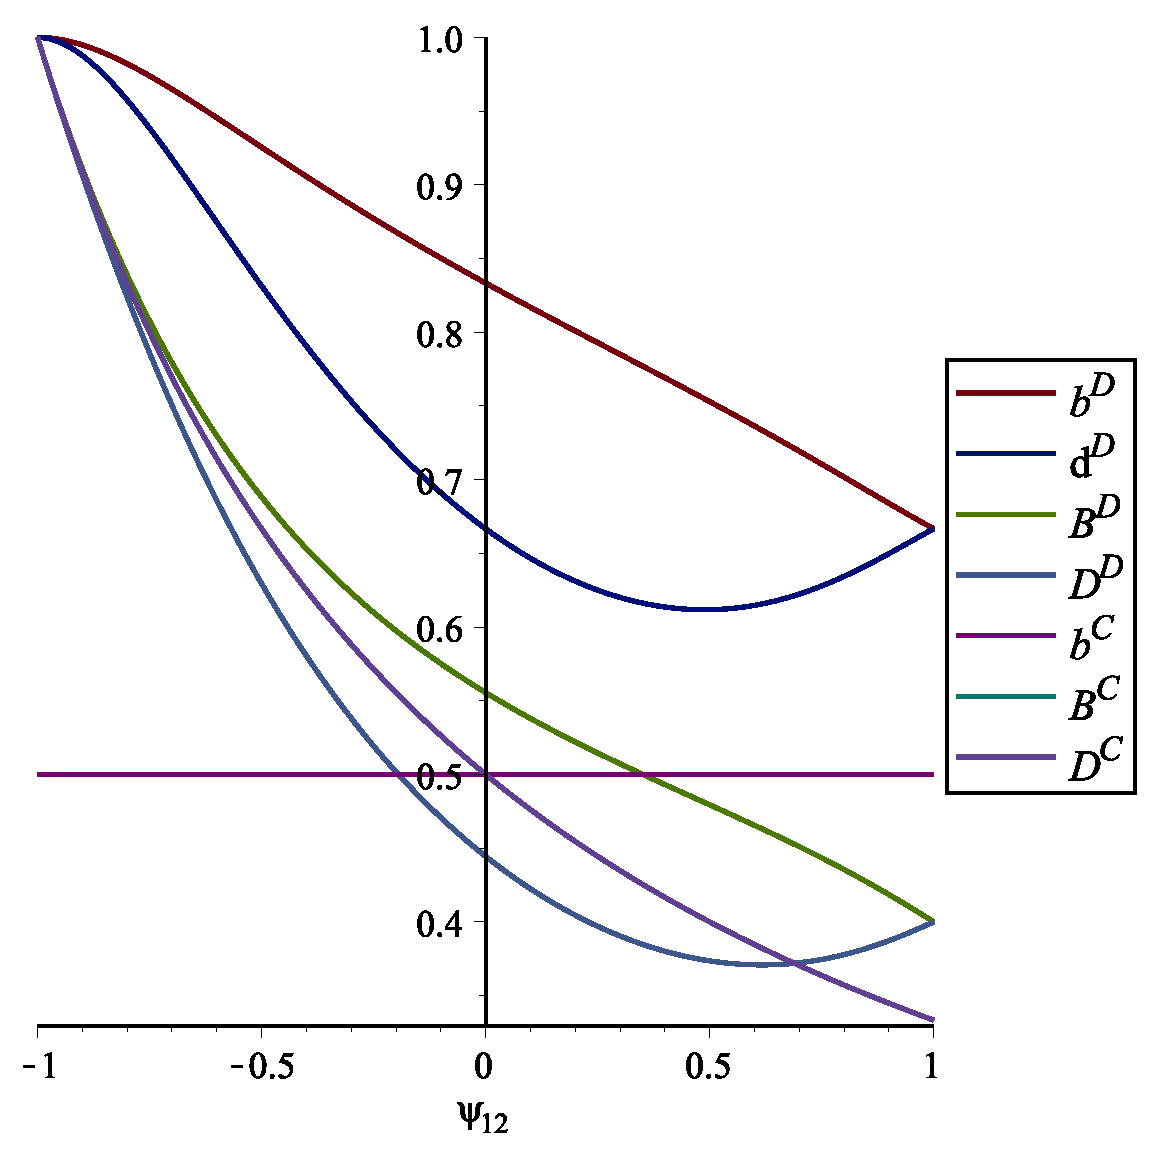
\includegraphics[width=0.65\textwidth]{gr1-eps-converted-to.pdf}
  \caption{Incentivos óptimos para distintos valores de $\psi_{12}$}
  \label{fig:app_incentivos_psi}
\end{figure}

\begin{figure}[htbp]
  \centering
  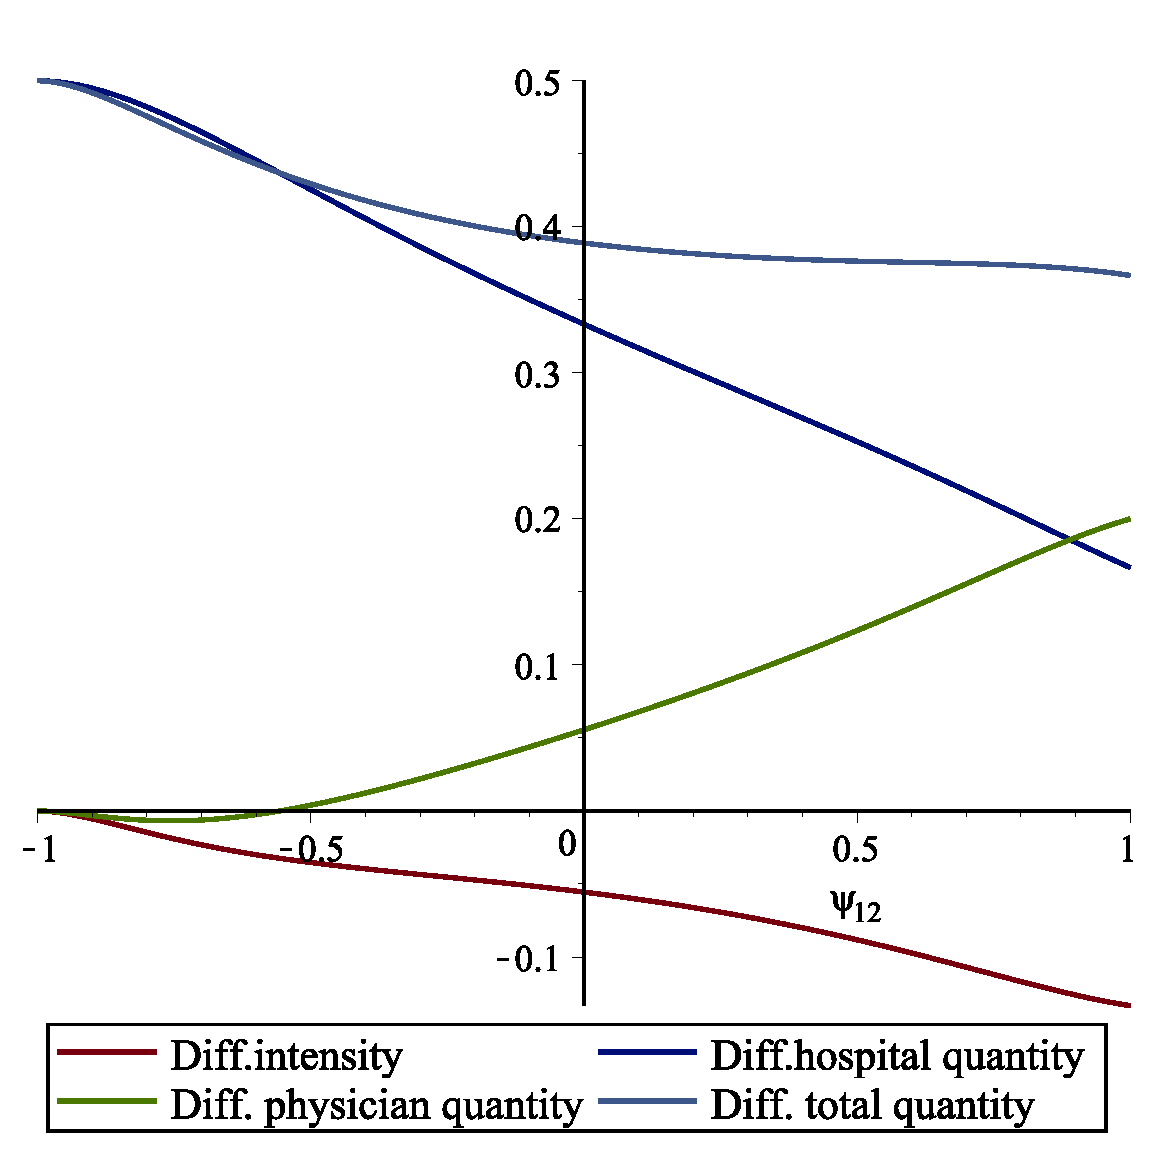
\includegraphics[width=0.65\textwidth]{gr2-eps-converted-to.pdf}
  \caption{Diferencial de esfuerzos para distintos valores de $\psi_{12}$}
  \label{fig:app_esfuerzos_psi}
\end{figure}

\section{Casos especiales: medición perfecta}

\begin{figure}[htbp]
  \centering
  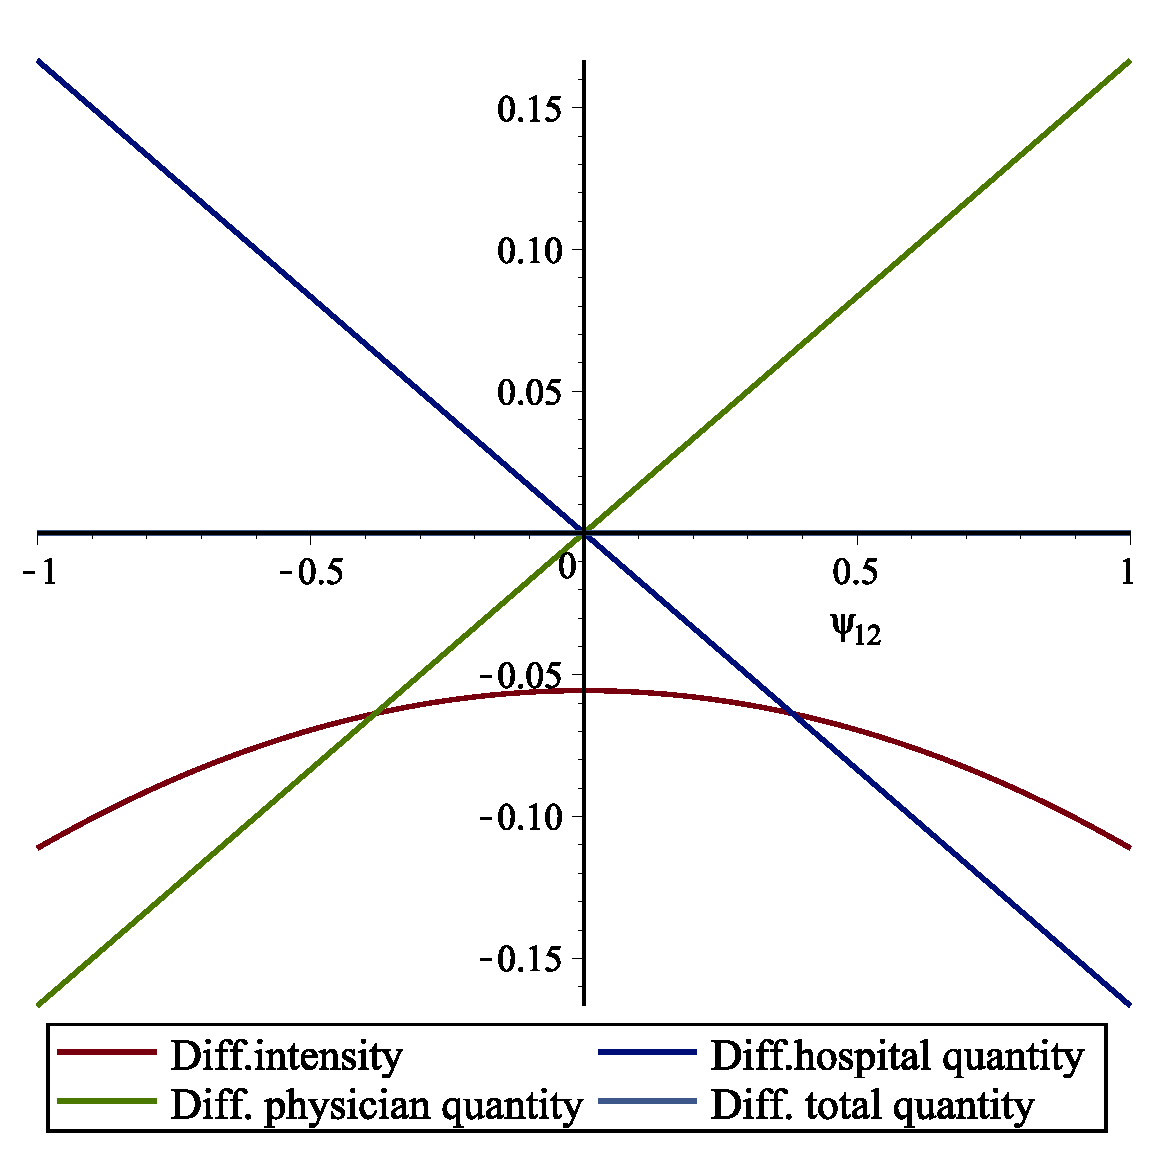
\includegraphics[width=0.65\textwidth]{gr3-eps-converted-to.pdf}
  \caption{Diferencial de esfuerzos dado $\sigma_1=0$ (medición perfecta de cantidad)}
  \label{fig:app_sigma1cero}
\end{figure}

\begin{figure}[htbp]
  \centering
  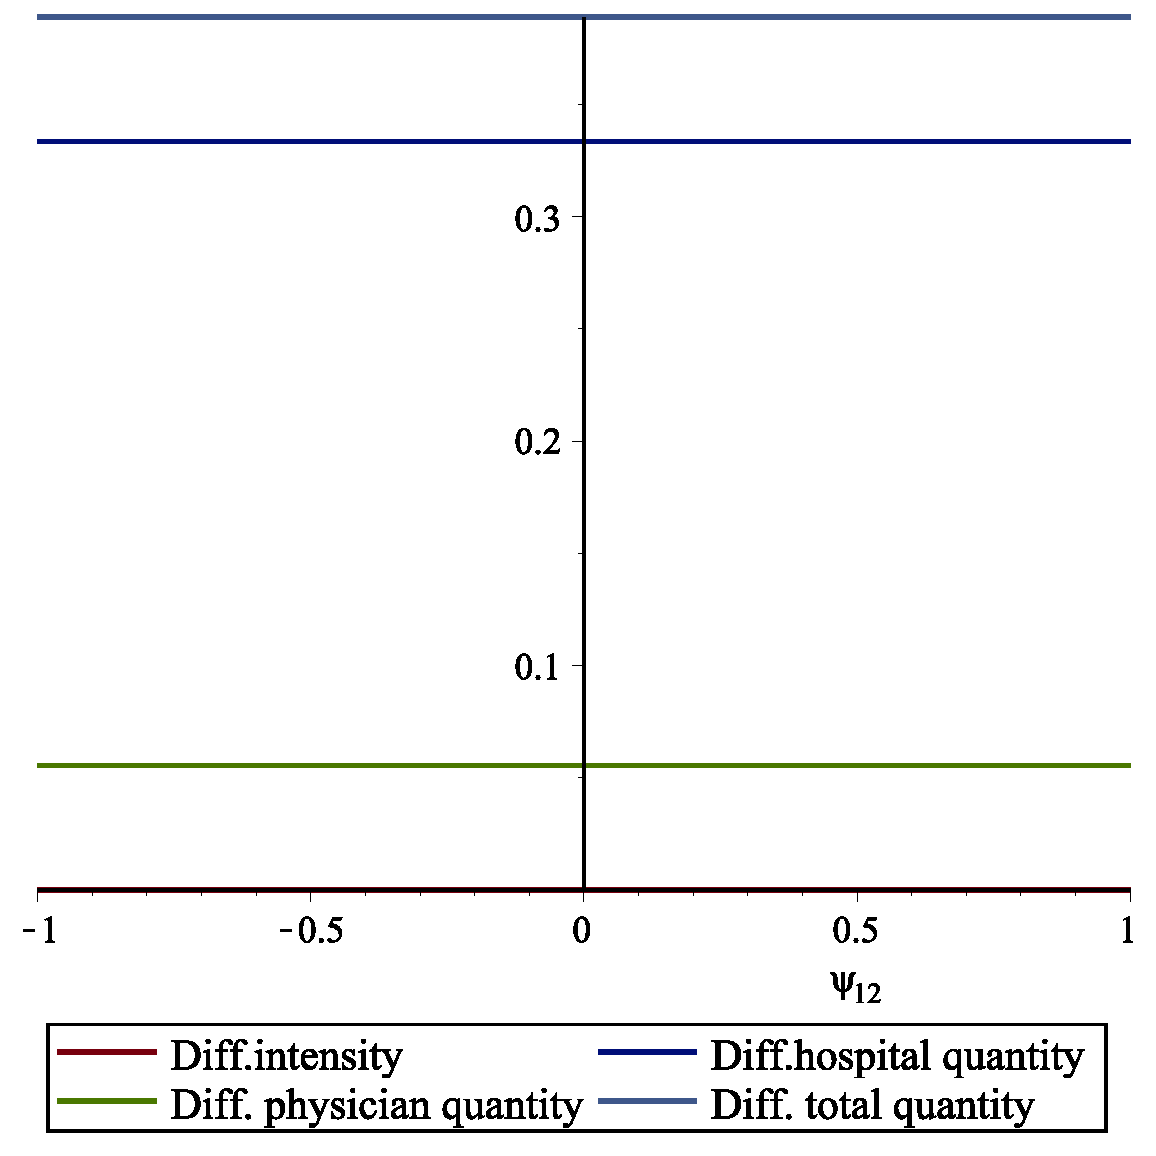
\includegraphics[width=0.65\textwidth]{gr4-eps-converted-to.pdf}
  \caption{Diferencial de esfuerzos dado $\sigma_2=0$ (medición perfecta de intensidad)}
  \label{fig:app_sigma2cero}
\end{figure}

\section{Variación en el ruido de cantidad (\texorpdfstring{$\sigma_1$}{sigma\_1})}

\begin{figure}[htbp]
  \centering
  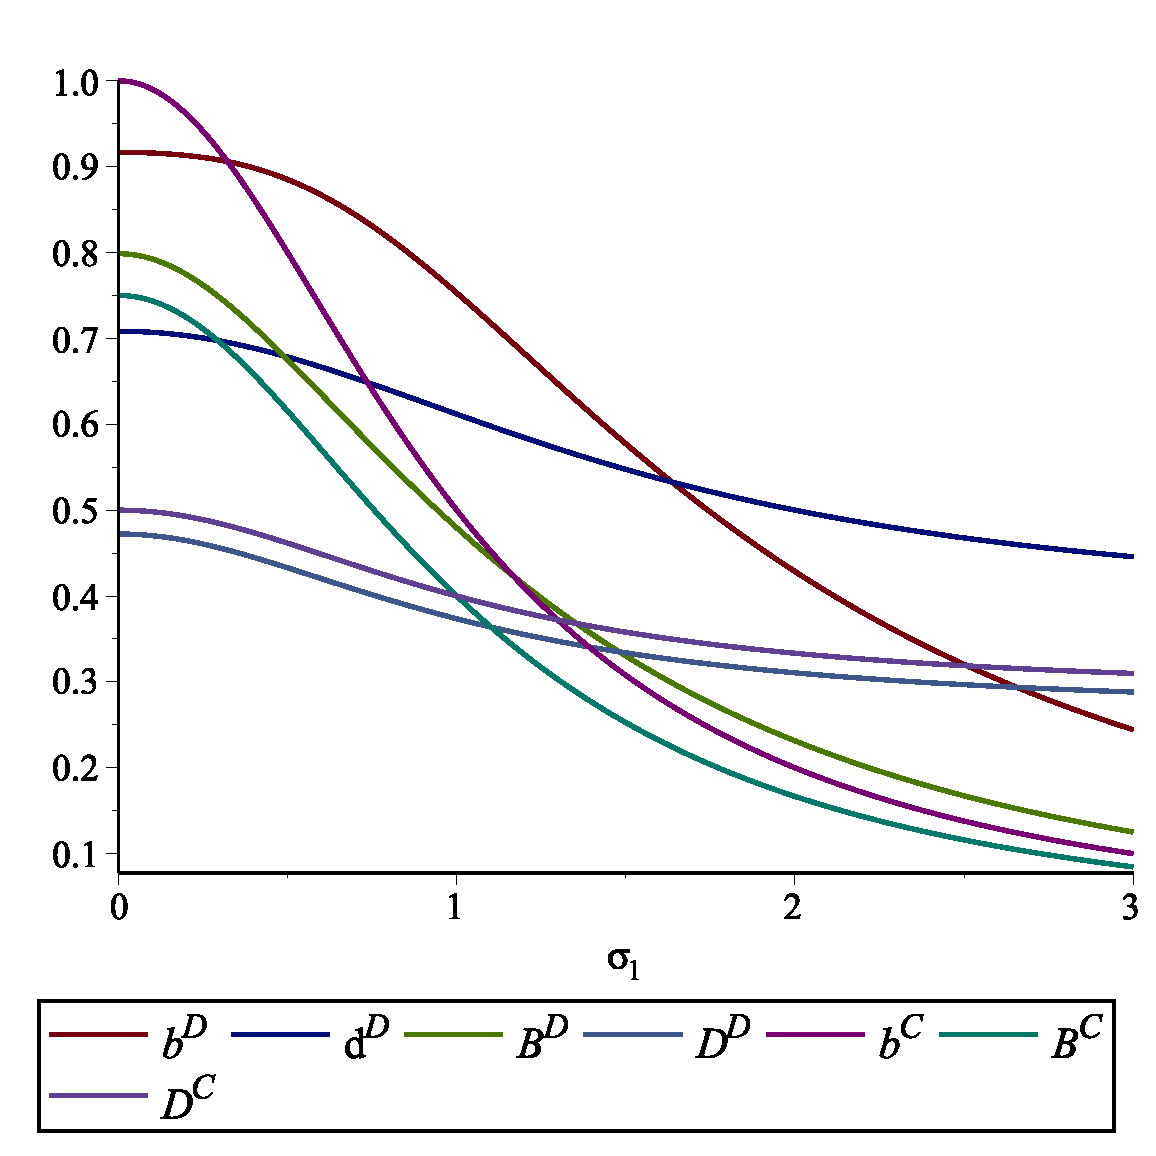
\includegraphics[width=0.65\textwidth]{gr5-eps-converted-to.pdf}
  \caption{Incentivos óptimos cuando aumenta $\sigma_1$ ($\psi_{12}=0.5$)}
  \label{fig:app_incentivos_sigma1}
\end{figure}

\begin{figure}[htbp]
  \centering
  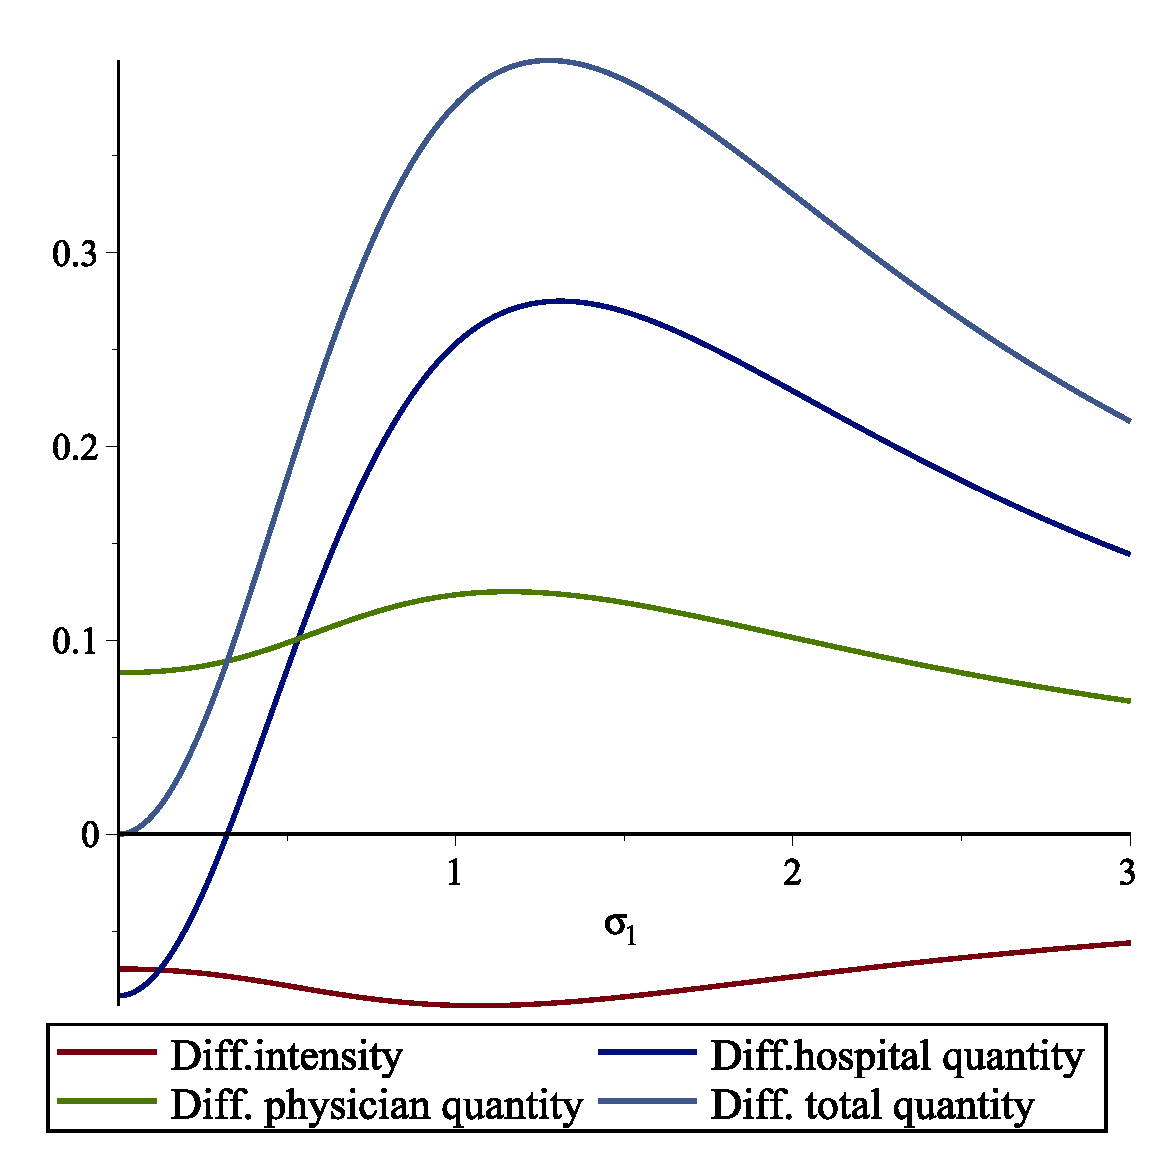
\includegraphics[width=0.65\textwidth]{gr6-eps-converted-to.pdf}
  \caption{Diferencial de esfuerzos cuando aumenta $\sigma_1$ ($\psi_{12}=0.5$)}
  \label{fig:app_esfuerzos_sigma1}
\end{figure}

\section{Variación en el ruido de intensidad (\texorpdfstring{$\sigma_2$}{sigma\_2})}

\begin{figure}[htbp]
  \centering
  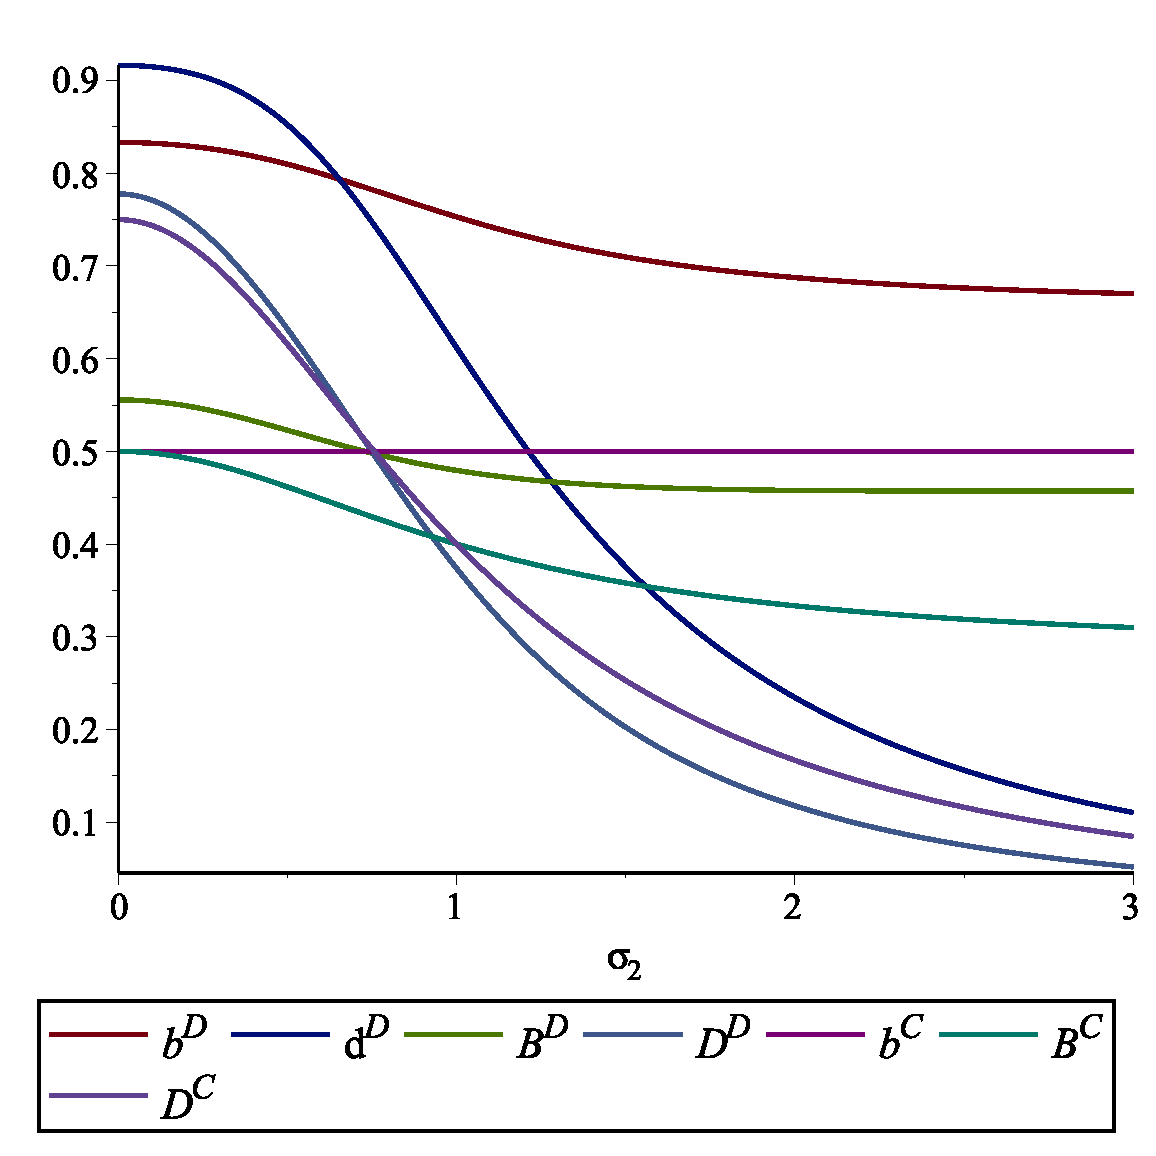
\includegraphics[width=0.65\textwidth]{gr7-eps-converted-to.pdf}
  \caption{Incentivos óptimos cuando aumenta $\sigma_2$ ($\psi_{12}=0.5$)}
  \label{fig:app_incentivos_sigma2}
\end{figure}

\begin{figure}[htbp]
  \centering
  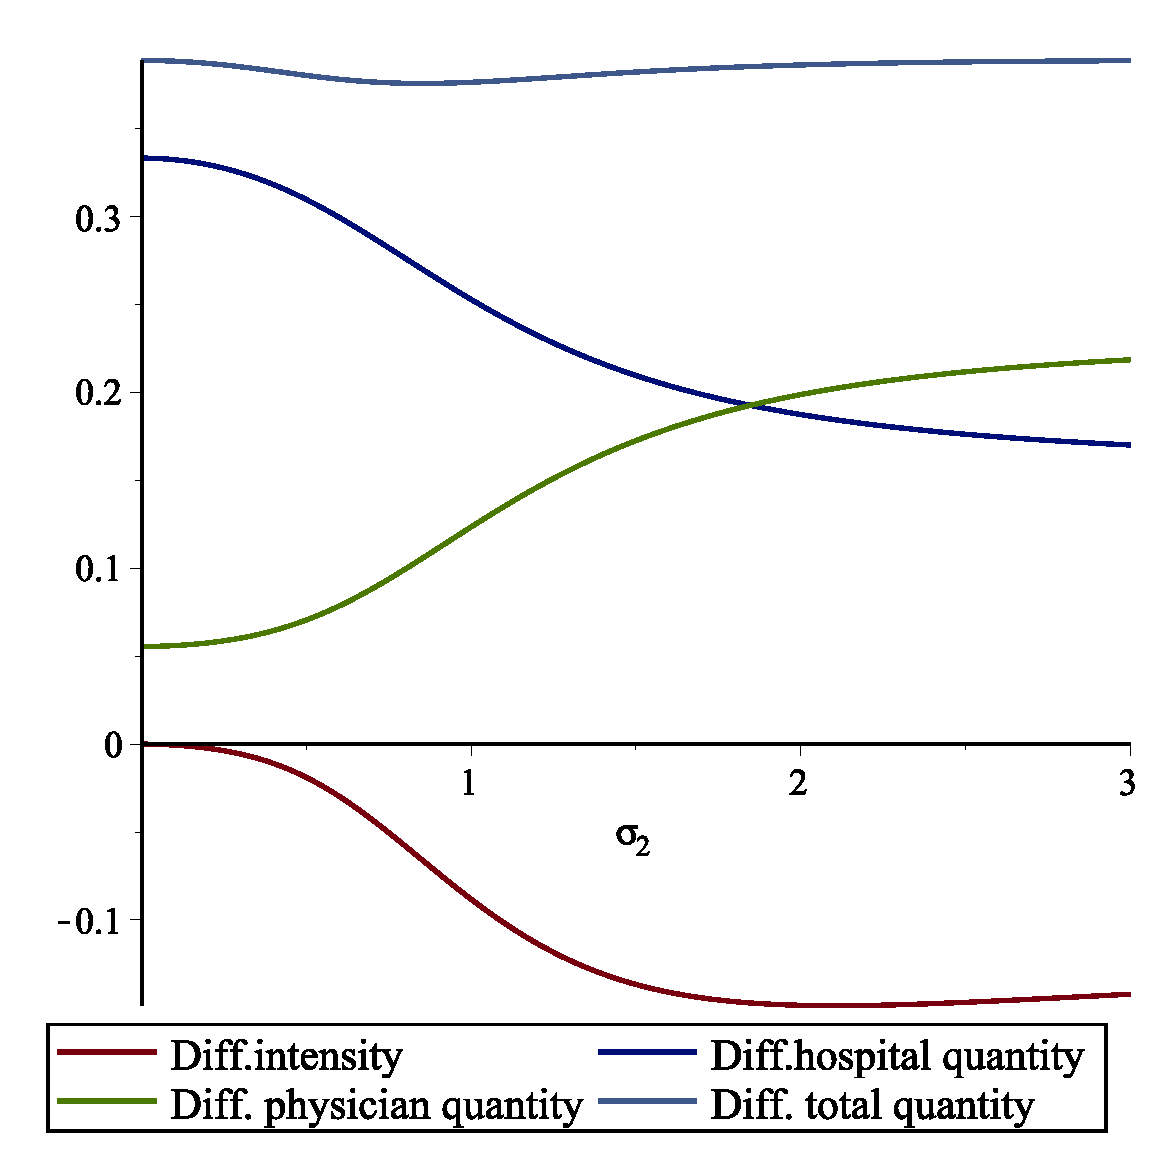
\includegraphics[width=0.65\textwidth]{gr8-eps-converted-to.pdf}
  \caption{Diferencial de esfuerzos cuando aumenta $\sigma_2$ (tareas sustitutas, $\psi_{12}=0.5$)}
  \label{fig:app_esfuerzos_sigma2_sust}
\end{figure}

\begin{figure}[htbp]
  \centering
  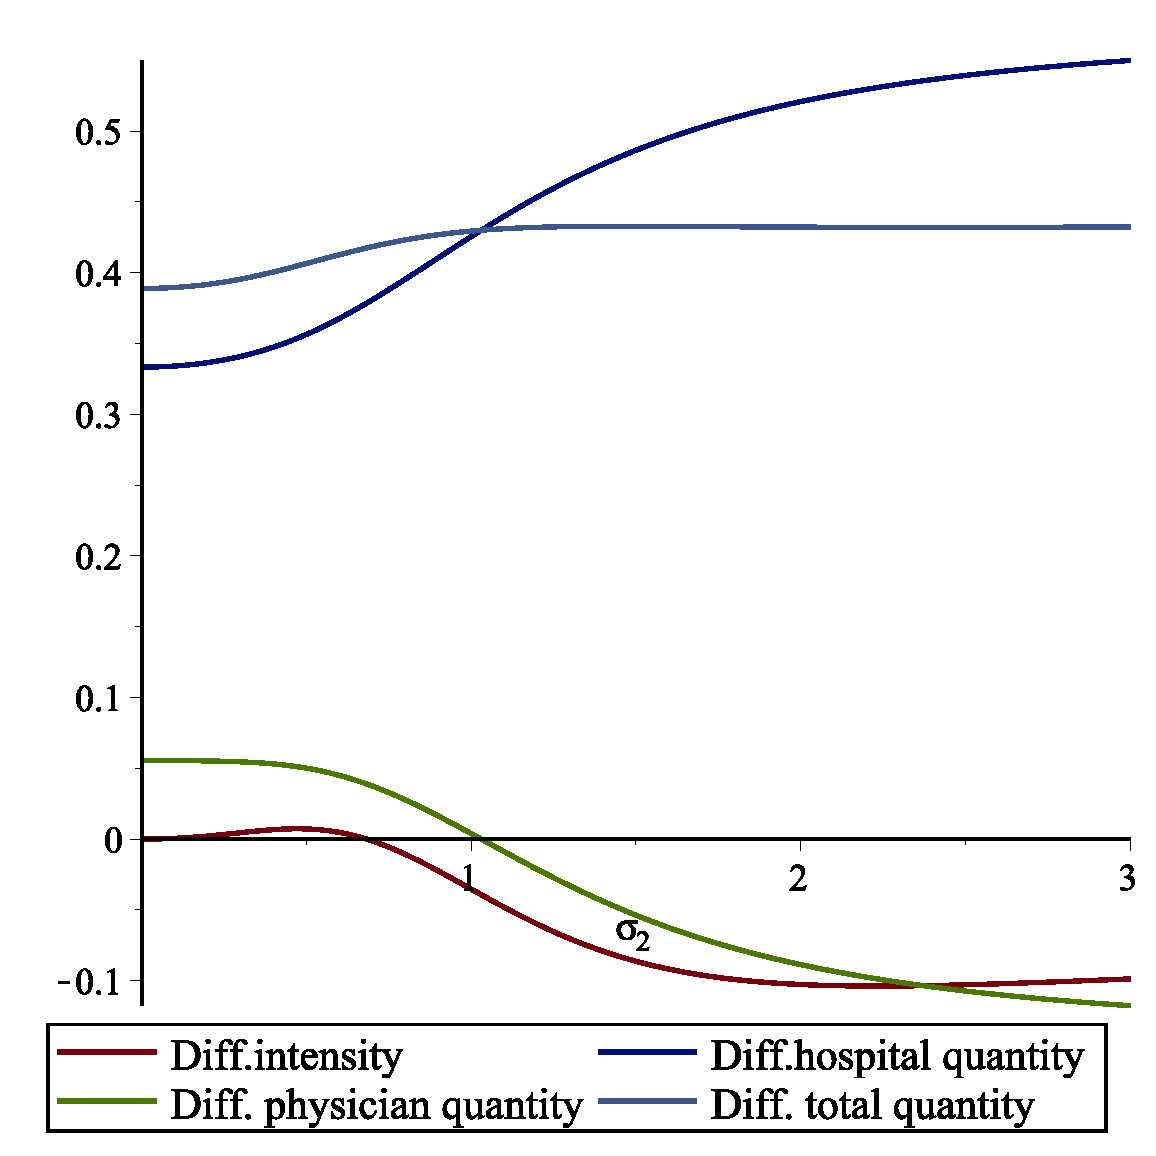
\includegraphics[width=0.65\textwidth]{gr9-eps-converted-to.pdf}
  \caption{Diferencial de esfuerzos cuando aumenta $\sigma_2$ (tareas complementarias, $\psi_{12}=-0.5$)}
  \label{fig:app_esfuerzos_sigma2_comp}
\end{figure}

Para tareas sustitutas ($\psi_{12}=0.5$), cuando la intensidad se mide sin ruido, los niveles de $t_2$ del médico son iguales en las dos estructuras y los esfuerzos sobre cantidad son mayores en la descentralizada. A medida que $\sigma_2$ crece, la intensidad se reduce en la descentralizada respecto de la centralizada, y los esfuerzos sobre cantidad también disminuyen, pero permanecen mayores en la descentralizada.

Para tareas complementarias ($\psi_{12}=-0.5$), se invierten los efectos iniciales sobre los esfuerzos en cantidad: el esfuerzo del médico disminuye y el del hospital aumenta en la descentralizada. Cuando $\sigma_2$ crece ligeramente por encima de $\sigma_1$, el esfuerzo del médico sobre cantidad pasa a ser mayor en la centralizada.


% ── ANEXO B: PIPELINE DE DATOS ───────────────────────────
\chapter{Construcción de variables y pipeline de datos}
\label{app:pipeline}

\section{Estructura del proyecto}

Los datos se procesan mediante un pipeline secuencial de scripts en R, cuyo código fuente está disponible en el repositorio del proyecto.\footnote{Repositorio privado durante el período de tesis.} La ruta raíz del proyecto es \texttt{G:/Mi unidad/SIAE 2010-2020/}.

\section{Orden de ejecución}

\begin{table}[htbp]
\centering
\caption{Pipeline de scripts R}
\label{tab:pipeline}
\small
\begin{tabular}{p{4cm}p{9cm}}
\toprule
\textbf{Script} & \textbf{Función} \\
\midrule
\texttt{00\_config.R} & Configuración central \\
\texttt{01\_exportar\_mapeo\_cnh.R} & Mapa NCODI $\leftrightarrow$ CNH \\
\texttt{02\_estandarizar\_nombres.R} & Renombra variables XML/TXT a nombres canónicos \\
\texttt{03\_unir\_modulos\_por\_anyo.R} & Une módulos SIAE por año \\
\texttt{04\_construir\_panel.R} & Apila años $\rightarrow$ panel longitudinal \\
\texttt{05\_construir\_casemix.R} & Case-mix (RF+LASSO), outputs ponderados, ShareQ \\
\texttt{06\_construir\_Ddesc\_pago.R} & $D^{desc}$, $pct^{SNS}$, inputs \\
\texttt{07\_construir\_intensidad.R} & $i_{diag}$ con bridges C1\_16 \\
\texttt{08\_auditoria\_variables.R} & Verificación de cobertura \\
\texttt{09\_crear\_df\_sfa.R} & Dataset reducido para SFA \\
\texttt{10\_descriptivos\_sfa.R} & Tablas descriptivas \\
\texttt{11\_estimar\_sfa.R} & Estimación 4 diseños + contrastes \\
\texttt{12\_robustez\_sfa.R} & 5 análisis de robustez \\
\texttt{13\_tests\_diagnosticos.R} & Tests formales \\
\bottomrule
\end{tabular}
\end{table}

\section{Armonización de formatos TXT y XML}
\label{sec:armonizacion_txt_xml_b}

El SIAE distribuyó sus microdatos en formato TXT con delimitador punto y coma para los años 2010--2015 y en formato XML (con estructura jerárquica de módulos) para los años 2016--2023. La transición entre formatos introdujo cambios en los nombres de variables, en la estructura de codificación de los módulos y en la presencia de nuevas variables no disponibles en el período TXT.

El proceso de armonización (script \texttt{02\_estandarizar\_nombres.R}) construye un \textit{mapping} canónico de nombres de variables que asocia cada variable del período TXT con su equivalente en el período XML. El mapping se construye en dos etapas. \textit{Primera}, una correspondencia exacta para las variables con nombre idéntico entre períodos (aproximadamente el 70\% del total). \textit{Segunda}, una correspondencia por \textit{fuzzy matching} basada en la distancia de Levenshtein normalizada entre nombres de variables, con umbral de similitud de 0.85, para las variables con nombre similar pero no idéntico. Las correspondencias obtenidas por fuzzy matching se validan manualmente contra la documentación metodológica del SIAE publicada por el Ministerio de Sanidad.

\section{Proceso de \textit{fuzzy matching} NCODI--CNH}
\label{sec:fuzzy_matching_cnh}

La vinculación entre las observaciones del SIAE (identificadas por el código NCODI de seis dígitos) y las del Catálogo Nacional de Hospitales (identificadas por el código CNH de siete dígitos) requiere un proceso de resolución de ambigüedades. El CNH publica anualmente un fichero con los hospitales activos; el SIAE mantiene su propio registro de centros activos. Los dos registros no son perfectamente congruentes porque el CNH incluye centros sin internamiento (consultorios, centros de salud) que el SIAE excluye, y porque algunos hospitales del SIAE tienen códigos NCODI que no aparecen en el CNH del mismo año.

El proceso de matching se realiza en tres pasos (script \texttt{01\_exportar\_mapeo\_cnh.R}):

\begin{enumerate}
  \item \textbf{Matching exacto por código}: para los hospitales con código NCODI que tiene una correspondencia directa y unívoca en el CNH del mismo año ($\approx$ 78\% de los casos).
  \item \textbf{Matching por nombre y municipio}: para los hospitales sin código exacto, se construye una cadena de texto combinando nombre y municipio del hospital y se calcula la distancia de Levenshtein normalizada entre la cadena del SIAE y la del CNH. Se acepta el match con similitud $\geq 0.80$ y se verifica que el municipio coincida al menos parcialmente.
  \item \textbf{Revisión manual}: para los casos con similitud $< 0.80$ o con ambigüedad (dos hospitales del CNH con similitud alta para el mismo NCODI), se realiza una revisión manual contra la página web del hospital y los registros históricos del SIAE.
\end{enumerate}

El resultado del matching cubre el 100\% de las observaciones del panel, con una cobertura del CNH del 96.4\% (el 3.6\% restante son hospitales que aparecen en el SIAE pero no en el CNH del año correspondiente, principalmente centros cerrados temporalmente o de nueva apertura; para estos, la dependencia funcional se imputa del año más cercano disponible).

\section{Armonización de variables \texorpdfstring{$i_{diag}$}{i\_diag}: validación de bridges C1\_16 v3}
\label{sec:bridges_v3}

En 2021, el módulo C1\_16 del SIAE cambió la denominación de las variables de procedimientos diagnósticos. Las equivalencias correctas utilizadas en la versión 3 del script de construcción son:
\begin{itemize}
  \item $\leq$2020: \texttt{biopsias\_hosp + biopsias\_CEP} $\rightarrow$ $\geq$2021: \texttt{totbiopsias}
  \item $\leq$2020: \texttt{tac\_hosp + tac\_CEP} $\rightarrow$ $\geq$2021: \texttt{tottac}
  \item $\leq$2020: \texttt{resonancia\_hosp + resonancia\_CEP} $\rightarrow$ $\geq$2021: \texttt{totresonancia}
  \item $\leq$2020: \texttt{Colonosopia} (sic, error tipográfico en variable original) $\rightarrow$ $\geq$2021: \texttt{Col\_hosp + Col\_Amb}
  \item Y análogamente para PET, Rx, SPECT, angiografía, gammacámara, mamografía, densitometría, broncoscopia y ERCP.
\end{itemize}

La versión 3 del bridge (\texttt{bridges\_C1\_16\_v3.csv}) corrige un error en la versión 2 que duplicaba las biopsias para los años 2016--2020, porque el módulo XML de esos años ya incluía la suma \texttt{hosp + CEP} en algunas variables pero no en otras, y la versión 2 sumaba incorrectamente las dos fuentes. La versión 3 verifica para cada variable y cada año si la suma de componentes \texttt{hosp + CEP} iguala o supera al total reportado, y solo agrega los componentes cuando es necesario.

Validación: la mediana de $i_{diag}$ es estable en el rango 8.1--9.5 durante 2010--2019, con una tendencia suave de aumento coherente con el progreso técnico diagnóstico. No se observa salto brusco en 2021 ni en 2016. La serie de 2016--2020 fue validada contra las estadísticas publicadas por el Ministerio de Sanidad sobre número de TAC y RNM realizados por hospital en esos años.

\section{Modelo de imputación de case-mix: detalles metodológicos}
\label{sec:casemix_imputacion}

Para los hospitales sin información directa de pesos GRD-APR (años 2016--2023 y hospitales no incluidos en el archivo de pesos 2010--2015), se estima un modelo de aprendizaje automático. Los detalles metodológicos son los siguientes.

\subsection{Variables predictoras}

Los predictores utilizados para la imputación del peso GRD medio son variables del SIAE disponibles para todos los hospitales y años del panel:

\begin{itemize}
  \item Proporción de altas con ingreso previo en UCI (\texttt{pct\_uci}): proxy de la gravedad media de los casos.
  \item Proporción de altas quirúrgicas sobre el total (\texttt{shareQ}): proxy de la complejidad del mix quirúrgico.
  \item Ratio de altas programadas sobre altas urgentes (\texttt{ratio\_prog\_urg}): proxy del grado de urgencia de la actividad.
  \item Índice tecnológico $K^T$: proxy de la sofisticación diagnóstica y terapéutica del hospital.
  \item Número de camas en funcionamiento ($K^C$): control de tamaño.
  \item Estancia media (número de estancias / número de altas): proxy de la complejidad media.
  \item Dummy de comunidad autónoma: captura diferencias regionales en la codificación GRD.
\end{itemize}

\subsection{Procedimiento de estimación}

Se entrena un modelo de Random Forest con 500 árboles (función \texttt{ranger} del paquete homónimo en R) sobre los datos disponibles del período 2010--2015 (246 hospitales, hasta 1.230 observaciones). El hiperparámetro \texttt{mtry} (número de variables a considerar en cada partición) se selecciona mediante validación cruzada con $k=5$ pliegues. El modelo LASSO (función \texttt{glmnet}) se estima sobre las mismas predictoras y se usa para comparación. El mejor modelo en términos de $R^2$ out-of-sample (Random Forest con $R^2 = 0.845$ vs. LASSO con $R^2 = 0.812$) se usa para la imputación.

La validación temporal hold-out usa los datos de 2014--2015 como test (entrena en 2010--2013). El $R^2 = 0.845$ indica que el modelo predice bien el peso GRD de los hospitales en años fuera de la muestra de entrenamiento. La varianza del error de imputación es mayor para los hospitales de pequeño tamaño (menos de 200 camas) y para los hospitales con cartera de servicios muy especializada (hospitales monoespecialistas de tumores, oftalmología, etc.), que quedan en su mayoría excluidos de la muestra por el filtro de actividad mínima.

El modelo se guarda como \texttt{casemix\_modelo\_B\_rf.rds} y se reutiliza sin re-entrenamiento en ejecuciones posteriores del pipeline. La caché del modelo RF permite reproducir exactamente los mismos valores imputados en cualquier ejecución del pipeline.


% ── ANEXO C: TABLAS COMPLEMENTARIAS ──────────────────────
\chapter{Tablas complementarias}
\label{app:tablas}

\section{Coeficientes de la frontera de producción}

Las tablas completas de coeficientes de la frontera de producción para los cuatro diseños se presentarán en la versión final del documento, una vez revisados los archivos \texttt{.rds} de modelos estimados. Los coeficientes principales son coherentes con los valores esperados:
\begin{itemize}
  \item Elasticidad del trabajo ($\hat{\beta}_1$): positiva y significativa en todos los modelos (rango 0.3--0.6).
  \item Elasticidad del capital-camas ($\hat{\beta}_2$): positiva y significativa (rango 0.2--0.5).
  \item Elasticidad del capital tecnológico ($\hat{\beta}_3$): positiva pero con mayor variabilidad entre modelos (rango 0.05--0.2).
  \item Progreso técnico ($\hat{\beta}_6$): positivo y significativo, indicando desplazamiento de la frontera hacia arriba en el tiempo.
  \item Aceleración/deceleración del progreso técnico ($\hat{\beta}_7$): negativo y pequeño, indicando una ligera ralentización del progreso en el período más reciente.
  \item Dummies de cluster: coeficientes positivos y crecientes con el nivel de complejidad, confirmando que los hospitales de mayor complejidad tienen una frontera de producción más alta. Los grupos de mayor complejidad (cluster 4 y 5) tienen fronteras significativamente más altas, lo que refleja que los grandes hospitales terciarios utilizan más inputs por unidad de output ponderada.
\end{itemize}

\section{Estadísticos descriptivos adicionales}
\label{sec:descriptivos_adicionales}

\begin{table}[htbp]
\centering
\caption{Distribución de observaciones por comunidad autónoma y estructura organizativa}
\label{tab:distribucion_ccaa}
\begin{threeparttable}
\small
\begin{tabular}{lrrrrr}
\toprule
\textbf{CCAA} & \textbf{Total obs.} & \textbf{Central.} & \textbf{Desc.}
  & \textbf{\% Desc.} & \textbf{TE$_q$ media} \\
\midrule
Andalucía       & 415 & 273 & 142 & 34.2 & 0.728 \\
Aragón          & 102 & 76  & 26  & 25.5 & 0.741 \\
Asturias        & 78  & 54  & 24  & 30.8 & 0.735 \\
Baleares        & 68  & 34  & 34  & 50.0 & 0.719 \\
Canarias        & 120 & 73  & 47  & 39.2 & 0.726 \\
Cantabria       & 44  & 38  & 6   & 13.6 & 0.748 \\
Castilla-LM     & 134 & 101 & 33  & 24.6 & 0.733 \\
Castilla-León   & 188 & 132 & 56  & 29.8 & 0.739 \\
Cataluña        & 621 & 248 & 373 & 60.1 & 0.718 \\
Com. Valenciana & 248 & 134 & 114 & 46.0 & 0.729 \\
Extremadura     & 58  & 51  & 7   & 12.1 & 0.744 \\
Galicia         & 176 & 108 & 68  & 38.6 & 0.736 \\
Madrid          & 542 & 187 & 355 & 65.5 & 0.715 \\
Murcia          & 93  & 63  & 30  & 32.3 & 0.731 \\
Navarra         & 52  & 28  & 24  & 46.2 & 0.743 \\
País Vasco      & 145 & 84  & 61  & 42.1 & 0.742 \\
La Rioja        & 23  & 18  & 5   & 21.7 & 0.748 \\
\midrule
Total           & 4.765 & 2.484 & 2.281 & 47.9 & 0.731 \\
\bottomrule
\end{tabular}
\begin{tablenotes}
  \small
  \item Muestra Diseño A. TE$_q$ media calculada por el estimador JLMS. La columna \% Desc. mide la proporción de observaciones con $D^{desc}=1$ en cada comunidad.
\end{tablenotes}
\end{threeparttable}
\end{table}

\section{Distribución de eficiencias técnicas por grupo de tamaño}

\begin{table}[htbp]
\centering
\caption{Eficiencias técnicas por grupo de complejidad (Diseño A)}
\label{tab:te_cluster}
\begin{threeparttable}
\small
\begin{tabular}{lrrrrrr}
\toprule
& \multicolumn{3}{c}{\textbf{Cantidad}} & \multicolumn{3}{c}{\textbf{Intensidad}} \\
\cmidrule(lr){2-4}\cmidrule(lr){5-7}
\textbf{Cluster} & Media & DE & $n$ & Media & DE & $n$ \\
\midrule
1 (menor complejidad) & 0.697 & 0.189 & 1.243 & 0.651 & 0.241 & 1.243 \\
2                     & 0.724 & 0.172 & 1.187 & 0.678 & 0.228 & 1.187 \\
3                     & 0.748 & 0.158 & 897   & 0.701 & 0.215 & 897   \\
4                     & 0.763 & 0.147 & 906   & 0.718 & 0.208 & 906   \\
5 (mayor complejidad) & 0.777 & 0.135 & 532   & 0.729 & 0.199 & 532   \\
\midrule
Total                 & 0.731 & 0.170 & 4.765 & 0.683 & 0.226 & 4.765 \\
\bottomrule
\end{tabular}
\begin{tablenotes}
  \small
  \item La clasificación en 5 grupos de complejidad sigue \citet{ministerio2007}. La mayor eficiencia en los hospitales de mayor complejidad es coherente con las economías de experiencia y especialización en los grandes hospitales terciarios.
\end{tablenotes}
\end{threeparttable}
\end{table}

\section{Notas sobre figuras}

Las figuras del Capítulo~\ref{ch:modelo} que representan los cronogramas de contratación (Figuras~\ref{fig:cronograma_c} y~\ref{fig:cronograma_d}) han sido implementadas mediante diagramas TikZ en español, sustituyendo los archivos EPS originales en inglés. Las figuras gr1--gr9 contienen únicamente símbolos matemáticos y etiquetas de ejes en notación LaTeX, por lo que no requieren traducción.


% ═══════════════════════════════════════════════════════════
% BIBLIOGRAFÍA
% ═══════════════════════════════════════════════════════════
\backmatter
\bibliographystyle{apalike}
\bibliography{referencias}

\end{document}
